\documentclass[12pt,a4paper]{book}

% Packages
\usepackage[utf8]{inputenc}
\usepackage[T1]{fontenc}
\usepackage[margin=2.5cm]{geometry}
\usepackage{graphicx}
\usepackage[table]{xcolor}
\usepackage{tikz}
\usepackage{titlesec}
\usepackage{fancyhdr}
\usepackage{tcolorbox}
\usepackage{enumitem}
\usepackage{fontawesome5}
\usepackage{setspace}
\usepackage{parskip}
\usepackage{mdframed}
\usepackage{booktabs}
\usepackage{array}
\usepackage{multirow}
\usepackage{tabularx}
\usepackage{makecell}
\usepackage{amssymb}

% Color Definitions
\definecolor{primary}{RGB}{139, 69, 19}      % Warm brown
\definecolor{secondary}{RGB}{210, 105, 30}   % Chocolate
\definecolor{accent}{RGB}{255, 140, 0}       % Dark orange
\definecolor{lightbg}{RGB}{255, 248, 240}    % Floral white
\definecolor{darktext}{RGB}{60, 40, 20}      % Dark brown
\definecolor{softpink}{RGB}{255, 182, 193}   % Light pink
\definecolor{sagegreen}{RGB}{138, 154, 91}   % Sage green
\definecolor{warmgray}{RGB}{128, 128, 105}   % Warm gray

% TikZ Libraries
\usetikzlibrary{shapes.geometric, arrows.meta, positioning, calc, shadows}

% tcolorbox Setup
\tcbuselibrary{skins,breakable}

% Custom Box Styles - FIXED with proper margins
\newtcolorbox{praktikbox}[1][]{
    enhanced,
    colback=lightbg,
    colframe=primary,
    fonttitle=\bfseries\large,
    title=#1,
    boxrule=2pt,
    arc=8pt,
    shadow={2pt}{-2pt}{0pt}{black!20},
    left=10pt, right=10pt, top=8pt, bottom=8pt,
    before skip=12pt, after skip=12pt,
    breakable
}

\newtcolorbox{tipbox}[1][Tips Praktis]{
    enhanced,
    colback=sagegreen!10,
    colframe=sagegreen!80!black,
    fonttitle=\bfseries,
    title=#1,
    boxrule=1.5pt,
    arc=5pt,
    left=10pt, right=10pt, top=8pt, bottom=8pt,
    before skip=10pt, after skip=10pt,
    breakable
}

\newtcolorbox{warningbox}[1][Peringatan]{
    enhanced,
    colback=accent!10,
    colframe=accent,
    fonttitle=\bfseries,
    title=#1,
    boxrule=1.5pt,
    arc=5pt,
    left=10pt, right=10pt, top=8pt, bottom=8pt,
    before skip=10pt, after skip=10pt,
    breakable
}

\newtcolorbox{exercisebox}[1][Latihan]{
    enhanced,
    colback=softpink!20,
    colframe=softpink!80!black,
    fonttitle=\bfseries,
    title=#1,
    boxrule=2pt,
    arc=8pt,
    left=10pt, right=10pt, top=8pt, bottom=8pt,
    before skip=10pt, after skip=10pt,
    breakable
}

\newtcolorbox{insightbox}{
    enhanced,
    colback=warmgray!10,
    colframe=warmgray,
    boxrule=1pt,
    arc=3pt,
    left=10pt, right=10pt, top=8pt, bottom=8pt,
    before skip=10pt, after skip=10pt,
    breakable
}

% Chapter Styling
\titleformat{\chapter}[display]
    {\normalfont\Huge\bfseries\color{primary}}
    {\tikz[remember picture,overlay] {
        \fill[primary] (0,0) rectangle (\paperwidth,3cm);
        \node[white,font=\Huge\bfseries] at (0.5\paperwidth,1.5cm) {\thechapter};
    }} 
    {1cm}
    {\Huge}
    [\vspace{0.5cm}]

\titleformat{\section}
    {\normalfont\Large\bfseries\color{secondary}}
    {\thesection}
    {1em}
    {}

\titleformat{\subsection}
    {\normalfont\large\bfseries\color{darktext}}
    {\thesubsection}
    {1em}
    {}

% Header and Footer
\pagestyle{fancy}
\fancyhf{}
\fancyhead[L]{\small\color{warmgray}Panduan Membangun Hubungan Sehat}
\fancyhead[R]{\small\color{warmgray}\thepage}
\fancyfoot[C]{\small\color{warmgray}Berdasarkan The Seven Principles for Making Marriage Work \& Wired for Dating}
\renewcommand{\headrulewidth}{0.5pt}
\renewcommand{\footrulewidth}{0.3pt}

% Custom Commands
\newcommand{\highlight}[1]{\textcolor{accent}{\textbf{#1}}}
\newcommand{\keyterm}[1]{\textcolor{primary}{\textbf{#1}}}
\newcommand{\emoji}[1]{\textcolor{accent}{$\bullet$}}

% Document Info
\title{
    \vspace{-2cm}
    {\Huge\bfseries\color{primary} PANDUAN PRAKTIS}\\[0.5cm]
    {\Huge\bfseries\color{secondary} Membangun Hubungan Sehat}\\[1cm]
    
\begin{tikzpicture}
        \draw[primary, line width=3pt] (0,0) -- (10,0);
    \end{tikzpicture}\\[0.5cm]
    {\Large\color{warmgray} Framework \& Tools Berdasarkan Sains}\\[0.3cm]
    {\large\color{warmgray} (The Seven Principles \& Wired for Dating)}
}

\author{
    \textbf{Rangkuman untuk Pasangan Modern}\\[0.3cm]
    {\small Edisi Bahasa Indonesia}
}

\date{\today}

\begin{document}

% Cover Page
\begin{titlepage}
\begin{tikzpicture}[remember picture, overlay]
    % Background gradient
    \fill[top color=lightbg, bottom color=softpink!30] 
        (current page.south west) rectangle (current page.north east);
    
    % Decorative elements
    \foreach \i in {1,...,20} {
        \fill[primary, opacity=0.1] 
            ($(current page.south west) + (rand*21cm, rand*29.7cm)$) 
            circle (0.3cm);
    }
    
    % Top bar
    \fill[primary] (current page.north west) rectangle ([yshift=-4cm]current page.north east);
    
    % Bottom bar
    \fill[secondary] (current page.south west) rectangle ([yshift=3cm]current page.south east);
\end{tikzpicture}

\vspace*{3cm}

\begin{center}
    {\fontsize{40}{48}\selectfont\bfseries\color{primary} PANDUAN}\\[0.3cm]
    {\fontsize{40}{48}\selectfont\bfseries\color{secondary} PRAKTIS}\\[1.5cm]
    
    
\begin{tikzpicture}
        \node[draw=primary, line width=2pt, rounded corners=15pt, 
              inner sep=20pt, fill=white, fill opacity=0.9] {
            \begin{minipage}{0.7\textwidth}
                \centering
                {\Huge\bfseries\color{darktext} Membangun\\[0.3cm]
                Hubungan Sehat}\\[0.5cm]
                {\Large\color{warmgray} Framework \& Tools\\
                untuk Pasangan Modern}
            \end{minipage}
        };
    \end{tikzpicture}
    
    \vspace{2cm}
    
    {\Large\color{primary}\faHeart\ \faBrain\ \faHandsHelping}\\[0.5cm]
    {\large\color{warmgray} Berdasarkan:\\[0.2cm]
    \textit{The Seven Principles for Making Marriage Work}\\
    \& \textit{Wired for Dating}}
    
    \vfill
    
    {\large\color{white} Edisi Bahasa Indonesia}
\end{center}
\end{titlepage}

% Table of Contents
\tableofcontents
\newpage

% Include Chapters
\chapter{Memahami Gaya Koneksi: Anchor, Island, Wave}

\begin{insightbox}
\textit{``Kunci hubungan yang sukses bukanlah menemukan pasangan sempurna, tapi memahami \highlight{bagaimana} kalian berdua terhubung. Ketika kamu mengenali gaya koneksimu dan pasanganmu, konflik bukan lagi personal --- itu hanya perbedaan wiring.''}
\end{insightbox}

\section{Apa itu Attachment Styles?}

\subsection{Sejarah Singkat}

Teori koneksi (attachment theory) pertama kali dikembangkan oleh psikolog John Bowlby pada tahun 1960-an. Bowlby mempelajari bagaimana bayi bereaksi saat dipisahkan dari caregiver-nya dan menemukan bahwa cara caregiver merespons kebutuhan bayi akan membentuk ``template'' hubungan untuk seumur hidup.

Dr. Stan Tatkin, dalam bukunya \textit{Wired for Dating}, menyederhanakan tiga dekade penelitian attachment menjadi tipe yang mudah dipahami: \highlight{Anchor} (Jangkar), \highlight{Island} (Pulau), dan \highlight{Wave} (Gelombang).

\begin{praktikbox}[Definisi Secure Functioning]
\keyterm{Secure functioning} adalah hubungan di mana:
\begin{itemize}
    \item Kalian saling menjaga keselamatan dan keamanan
    \item Sensitif terhadap kebutuhan satu sama lain
    \item Cepat memperbaiki kesalahan yang terjadi
    \item Berkolaborasi sebagai tim
    \item Menjalankan \textit{true mutuality} --- apa yang baik untukku juga baik untukmu
\end{itemize}
\end{praktikbox}

\section{Anchor (Jangkar): Dua Lebih Baik dari Satu}

\subsection{Siapa itu Anchor?}

Anchor adalah tipe yang paling \textit{secure} dalam hubungan. Mereka tumbuh dengan caregiver yang responsif, sehingga internalize bahwa dunia adalah tempat yang aman dan orang lain bisa diandalkan.

\begin{center}
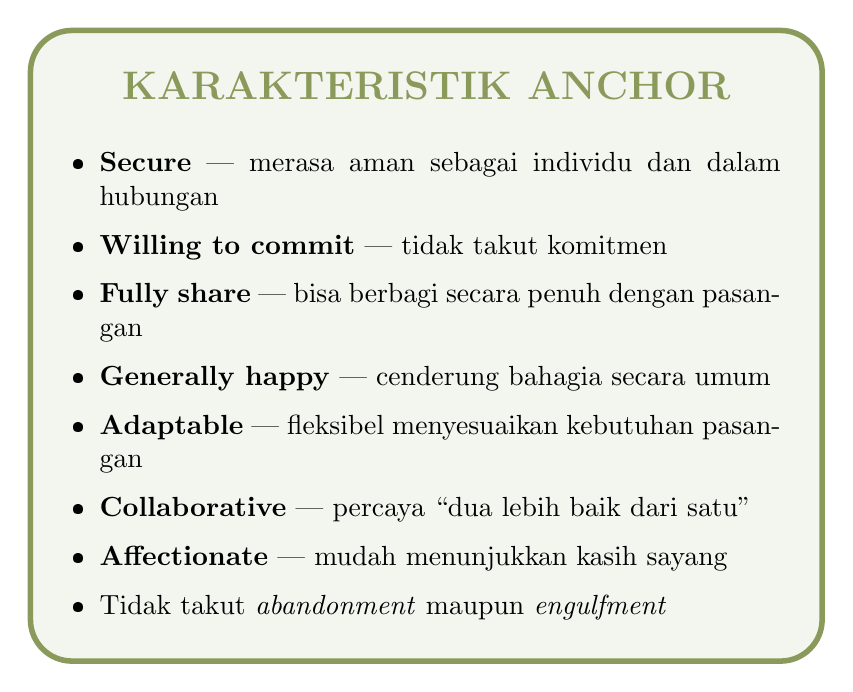
\begin{tikzpicture}[
    anchorbox/.style={draw=sagegreen, line width=2pt, rounded corners=15pt, 
                   fill=sagegreen!10, minimum width=10cm, inner sep=15pt}
]
    \node[anchorbox] (box) {
        \begin{minipage}{9cm}
            \centering
            {\Large\bfseries\color{sagegreen} KARAKTERISTIK ANCHOR}\\[0.5cm]
            \begin{itemize}[leftmargin=*, itemsep=0.2cm]
                \item \textbf{Secure} --- merasa aman sebagai individu dan dalam hubungan
                \item \textbf{Willing to commit} --- tidak takut komitmen
                \item \textbf{Fully share} --- bisa berbagi secara penuh dengan pasangan
                \item \textbf{Generally happy} --- cenderung bahagia secara umum
                \item \textbf{Adaptable} --- fleksibel menyesuaikan kebutuhan pasangan
                \item \textbf{Collaborative} --- percaya ``dua lebih baik dari satu''
                \item \textbf{Affectionate} --- mudah menunjukkan kasih sayang
                \item Tidak takut \textit{abandonment} maupun \textit{engulfment}
            \end{itemize}
        \end{minipage}
    };
\end{tikzpicture}
\end{center}

\subsection{Anchor sebagai Anak}

Anchor berasal dari lingkungan keluarga yang:
\begin{enumerate}
    \item Menempatkan \textbf{hubungan di atas segalanya}
    \item Setidaknya satu caregiver yang \textbf{fully present} dan tersedia
    \item Caregiver \textbf{affectionate} --- suka memeluk, mencium, mengayun
    \item Menghabiskan waktu \textbf{face-to-face, eye-to-eye, skin-to-skin}
    \item Saat anak marah/sedih, caregiver \textbf{menenangkan dengan efektif}
    \item Tidak membeli anak dengan hadiah saat anak emosional
    \item Melihat anak secara akurat dan mengenalnya dengan dalam
    \item Menghargai \textbf{dependency} dan \textbf{autonomy} secara seimbang
\end{enumerate}

\begin{tipbox}[Bedah Perilaku Anchor]
\textbf{Sehari-hari:}
\begin{itemize}
    \item Mudah meminta bantuan dan menerima bantuan
    \item Tidak merasa terancam jika pasangan butuh ruang
    \item Tidak merasa cekik jika pasangan ingin dekat
    \item Bisa sendiri atau bersama pasangan dengan sama nyamannya
\end{itemize}

\textbf{Dalam Konflik:}
\begin{itemize}
    \item Mencari solusi win-win
    \item Tidak defensive secara berlebihan
    \item Tetap terhubung meski sedang marah
    \item Bisa mengatakan ``aku memilihmu'' tanpa ragu
\end{itemize}
\end{tipbox}

\subsection{Apakah Anchor Sempurna?}

\textbf{Tidak!} Anchor juga bisa:
\begin{itemize}
    \item Membuat lelucon yang tidak lucu
    \item Terlambat ke janji
    \item Lupa mematikan lampu
    \item Menyebalkan dalam hal-hal kecil
\end{itemize}

Tapi mereka \textbf{resilient} --- punya sumber daya internal yang kuat karena merasa \textit{tethered} (terikat) pada seseorang. Mereka tidak hidup sebagai \textit{lone wolves}.

\section{Island (Pulau): Aku Bisa Melakukannya Sendiri}

\subsection{Paradoks Island}

Island adalah tipe yang paling \textbf{kontradiktif}. Di permukaan, mereka tampak:
\begin{itemize}
    \item Mandiri
    \item Tidak butuh siapa-siapa
    \item Low maintenance
\end{itemize}

Tapi \textbf{paradoksnya}: Island seringkali adalah tipe yang \textbf{paling membutuhkan} pasangan, hanya saja mereka \textit{tidak tahu} cara menerima kebutuhan itu.

\begin{center}
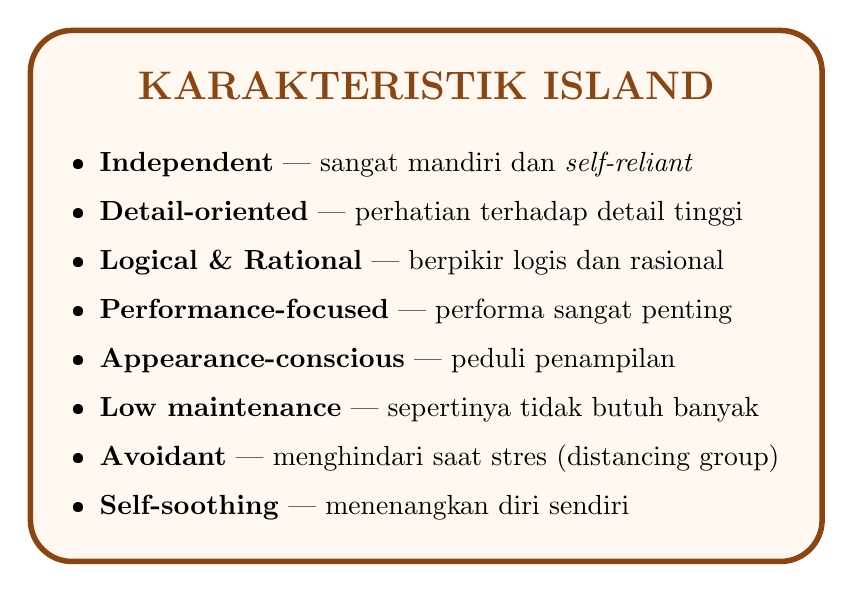
\begin{tikzpicture}[
    island/.style={draw=primary, line width=2pt, rounded corners=15pt, 
                   fill=lightbg, minimum width=10cm, inner sep=15pt}
]
    \node[island] (box) {
        \begin{minipage}{9cm}
            \centering
            {\Large\bfseries\color{primary} KARAKTERISTIK ISLAND}\\[0.5cm]
            \begin{itemize}[leftmargin=*, itemsep=0.2cm]
                \item \textbf{Independent} --- sangat mandiri dan \textit{self-reliant}
                \item \textbf{Detail-oriented} --- perhatian terhadap detail tinggi
                \item \textbf{Logical \& Rational} --- berpikir logis dan rasional
                \item \textbf{Performance-focused} --- performa sangat penting
                \item \textbf{Appearance-conscious} --- peduli penampilan
                \item \textbf{Low maintenance} --- sepertinya tidak butuh banyak
                \item \textbf{Avoidant} --- menghindari saat stres (distancing group)
                \item \textbf{Self-soothing} --- menenangkan diri sendiri
            \end{itemize}
        \end{minipage}
    };
\end{tikzpicture}
\end{center}

\subsection{Island sebagai Anak}

Island tumbuh dalam keluarga yang:
\begin{enumerate}
    \item Menekankan \textbf{performa, kecerdasan, bakat, penampilan}
    \item \textbf{Menghambat dependency} --- anggap kebutuhan itu aib
    \item Caregiver bisa \textbf{dingin, meremehkan, atau dismissive}
    \item Saat anak sedih, caregiver memberi \textbf{uang/mainan} alih-alih perhatian
    \item Caregiver \textbf{menarik diri, aloof, atau tidak tersedia}
    \item Caregiver \textbf{mementingkan kebutuhan sendiri} di atas hubungan
    \item Saat anak ketakutan di malam hari, caregiver \textbf{tidak responsif}
    \item Saat anak kesakitan, caregiver \textbf{mengabaikan, mengkritik, atau meremehkan}
\end{enumerate}

\begin{warningbox}[Kenapa Island Tampak ``Baik-baik Saja''?]
Island anak seringkali tampak \textit{well-adjusted} karena:
\begin{itemize}
    \item Mereka bermain sendiri dengan bahagia
    \item Tidak menunjukkan kebutuhan secara terbuka
    \item Tampak ``dewasa'' untuk usianya
\end{itemize}

Tapi di dalam, mereka memiliki \textbf{self yang rapuh} yang tidak tahu cara menangani pikiran dan perasaan stres.
\end{warningbox}

\subsection{Mengapa Island Menjauh (Distancing)?}

Saat stres, Island masuk ke \keyterm{distancing group} --- menjauh dari orang lain. Ini karena:

\begin{enumerate}
    \item \textbf{Hubungan dekat = Stres:} Hubungan intim membawa terlalu banyak ancaman yang kabur
    \item \textbf{Self-soothing otomatis:} Refleks mereka adalah menenangkan diri sendiri, bukan mencari pasangan
    \item \textbf{Takut kehilangan otonomi:} Island sangat sensitif terhadap perasaan terjebak
    \item \textbf{Pengalaman keluarga:} Dari kecil, isolasi = relief, bukan kehilangan
\end{enumerate}

\begin{tipbox}[Deteksi Island dalam Hubungan]
\textbf{Warning signs:}
\begin{itemize}
    \item Sering lupa janji atau ``lupa'' memberi tahu kemana perginya
    \item Saat ada masalah, menghilang atau merenung sendiri
    \item Sulit bertransisi dari aktivitas solo ke interaksi dengan pasangan
    \item Saat dipeluk terlalu lama, mulai gelisah
    \item Saat ditanya ``Kamu kenapa?'', jawabannya ``Tidak apa-apa''
\end{itemize}

\textbf{Strengths:}
\begin{itemize}
    \item Sangat bisa diandalkan dalam krisis
    \item Tidak membuat drama yang tidak perlu
    \item Menghargai waktu sendiri pasangan
    \item Produktif dan fokus pada pekerjaan
\end{itemize}
\end{tipbox}

\section{Wave (Gelombang): Aku Tidak Bisa Tanpamu}

\subsection{Siapa itu Wave?}

Wave adalah tipe yang paling \textbf{emotional} dan \textbf{relational}. Mereka hidup untuk koneksi, tapi seringkali takut akan kehilangannya.

\begin{center}
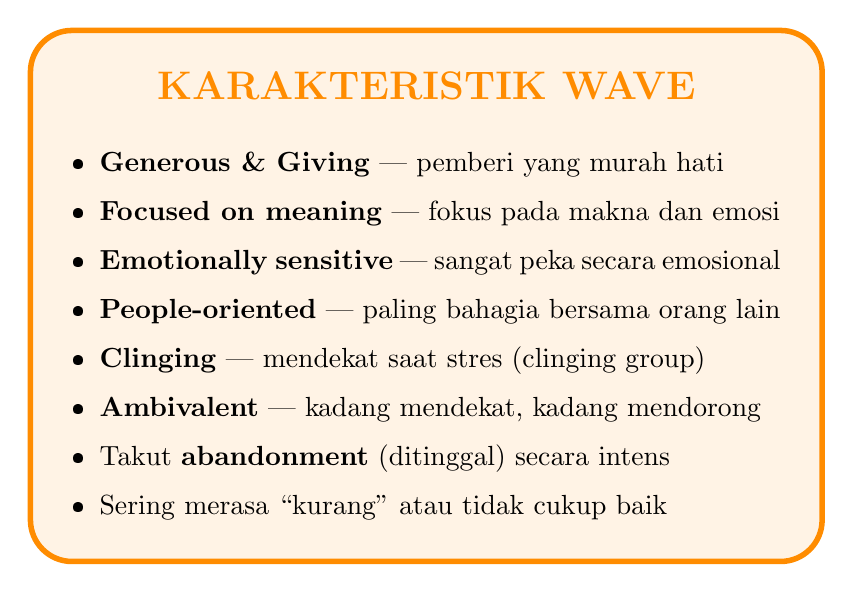
\begin{tikzpicture}[
    wave/.style={draw=accent, line width=2pt, rounded corners=15pt, 
                 fill=accent!10, minimum width=10cm, inner sep=15pt}
]
    \node[wave] (box) {
        \begin{minipage}{9cm}
            \centering
            {\Large\bfseries\color{accent} KARAKTERISTIK WAVE}\\[0.5cm]
            \begin{itemize}[leftmargin=*, itemsep=0.2cm]
                \item \textbf{Generous \& Giving} --- pemberi yang murah hati
                \item \textbf{Focused on meaning} --- fokus pada makna dan emosi
                \item \textbf{Emotionally sensitive} --- sangat peka secara emosional
                \item \textbf{People-oriented} --- paling bahagia bersama orang lain
                \item \textbf{Clinging} --- mendekat saat stres (clinging group)
                \item \textbf{Ambivalent} --- kadang mendekat, kadang mendorong
                \item Takut \textbf{abandonment} (ditinggal) secara intens
                \item Sering merasa ``kurang'' atau tidak cukup baik
            \end{itemize}
        \end{minipage}
    };
\end{tikzpicture}
\end{center}

\subsection{Wave sebagai Anak}

Wave tumbuh dalam keluarga yang:
\begin{enumerate}
    \item Caregiver \textbf{membutuhkan perhatian anak} untuk merasa lebih baik (role reversal)
    \item Caregiver \textbf{kadang sangat perhatian, kadang tidak tersedia} (inconsistent)
    \item Saat anak sedih, caregiver \textbf{memfokuskan pada emosi sendiri}
    \item Caregiver \textbf{mudah tersinggung, sering kewalahan, atau menghukum}
    \item Caregiver \textbf{membuat anak sebagai ally} melawan pasangannya
    \item Saat anak ketakutan di malam hari, caregiver \textbf{tidak menenangkan dengan efektif}
\end{enumerate}

\subsection{Paradoks Wave: Mendekat tapi Mendorong}

Wave punya pola yang membingungkan:
\begin{enumerate}
    \item \textbf{Cling} --- mendekat, ingin perhatian, manja
    \item \textbf{Push away} --- tiba-tiba marah, menyindir, atau mengancam pergi
    \item \textbf{Test} --- ``Kalau aku pergi, apakah dia mengejar?''
    \item \textbf{Want pursuit} --- sebenarnya ingin pasangan mengejar dan membuktikan cinta
\end{enumerate}

\begin{praktikbox}[Mengapa Wave Melakukan Ini?]
Ini adalah \textbf{test of love}. Wave belajar dari pengalaman masa kecil bahwa cinta itu:
\begin{itemize}
    \item Tidak konsisten
    \item Harus diperjuangkan
    \item Bisa hilang kapan saja
\end{itemize}

Jadi mereka menciptakan situasi untuk membuktikan bahwa ``Dia benar-benar peduli'' dengan membuat pasangan \textbf{mengejar} mereka.
\end{praktikbox}

\section{Quiz Komprehensif: Kamu Tipe Apa?}

\begin{exercisebox}[Attachment Style Quiz --- Versi Detail]
\textbf{Petunjuk:} Untuk setiap pertanyaan, pilih jawaban yang \textit{paling sering} menggambarkan dirimu. Jujur pada dirimu sendiri --- ini untuk pemahaman, bukan penilaian.

\subsection*{BAGIAN A: Masa Kecil (Sebelum Usia 13)}

\textbf{1. Kapan kamu sedih atau menangis, bagaimana orang tua/caregiver bereaksi?}
\begin{itemize}
    \item[A] Datang, memeluk, menenangkan dengan efektif tanpa menghakimi
    \item[B] Memberikan mainan/uang, atau mengatakan ``Jangan menangis'', ``Besar kok nangis''
    \item[C] Kadang memeluk dengan penuh kasih, kadang bilang ``Ah, gitu aja nangis''
\end{itemize}

\textbf{2. Bagaimana budaya keluargamu tentang kebutuhan dan ketergantungan?}
\begin{itemize}
    \item[A] Normal dan diterima untuk saling bergantung dan dimanja
    \item[B] Ketergantungan dianggap kelemahan. ``Kamu harus mandiri''
    \item[C] Kamu diharapkan menjadi ``penyelamat'' atau tempat curhat orang tua
\end{itemize}

\textbf{3. Seberapa sering kamu merasa benar-benar ``dilihat'' dan dipahami oleh orang tua?}
\begin{itemize}
    \item[A] Sering --- mereka benar-benar tahu siapa aku
    \item[B] Jarang --- lebih fokus pada nilai/penampilanku
    \item[C] Kadang-kadang saja, tergantung mood mereka
\end{itemize}

\textbf{4. Saat kamu takut di malam hari dan memanggil, apa yang terjadi?}
\begin{itemize}
    \item[A] Seseorang datang dan menenangkan
    \item[B] Disuruh tidur sendiri, atau diberi lampu/mainan
    \item[C] Kadang ditemani, kadang disuruh ``jangan manja''
\end{itemize}

\textbf{5. Bagaimana cara orang tuamu menunjukkan kasih sayang?}
\begin{itemize}
    \item[A] Pelukan, ciuman, waktu berkualitas bersama
    \item[B] Hadiah, uang, atau prestasi yang dihargai
    \item[C] Kadang sangat manja, kadang dingin/marah
\end{itemize}

\subsection*{BAGIAN B: Dalam Hubungan Dewasa}

\textbf{6. Saat pasangan ingin bicara serius tentang hubungan, biasanya kamu:}
\begin{itemize}
    \item[A] Dengan senang hati --- ini memperkuat koneksi kita
    \item[B] Merasa ingin menjauh, menunda, atau menghilang
    \item[C] Senang, tapi takut dia akan marah besar atau pergi
\end{itemize}

\textbf{7. Bagaimana cara kamu ``recharge'' energi?}
\begin{itemize}
    \item[A] Bisa sama baiknya sendiri atau bersama pasangan
    \item[B] \textbf{Harus} punya waktu sendiri --- ``me-time'' adalah wajib
    \item[C] Butuh bersama pasangan --- sendiri membuatku cemas/ kosong
\end{itemize}

\textbf{8. Saat ada konflik, kamu cenderung:}
\begin{itemize}
    \item[A] Mencari solusi bersama, tetap terhubung meski marah
    \item[B] Menarik diri, merenung sendiri, atau menghindari
    \item[C] Mengejar, membuat dramatis, atau kadang mengancam putus
\end{itemize}

\textbf{9. Saat pasangan tidak membalas pesan dengan cepat, kamu:}
\begin{itemize}
    \item[A] Menganggap dia sibuk, tidak memikirkannya terus
    \item[B] Senang --- aku juga butuh ruang
    \item[C] Cemas, kepikiran terus, mungkin dia marah atau tidak cinta lagi
\end{itemize}

\textbf{10. Bagaimana perasaanmu tentang komitmen jangka panjang?}
\begin{itemize}
    \item[A] Nyaman dan positif --- aku ingin membangun sesuatu yang kuat
    \item[B] Was-was --- takut kehilangan kebebasan dan independensiku
    \item[C] Ingin sekali, tapi takut ditinggal atau tidak dicintai sepenuhnya
\end{itemize}

\subsection*{SCORING}

\begin{center}
\renewcommand{\arraystretch}{1.3}
\begin{tabular}{|c|c|c|c|}
\hline
\rowcolor{primary!20}
\textbf{Jawaban} & \textbf{Anchor} & \textbf{Island} & \textbf{Wave} \\
\hline
A & \checkmark & & \\
\hline
B & & \checkmark & \\
\hline
C & & & \checkmark \\
\hline
\end{tabular}
\end{center}

\textbf{Interpretasi:}
\begin{itemize}
    \item \textbf{7-10 A:} Kamu adalah \textbf{ANCHOR} yang kuat
    \item \textbf{7-10 B:} Kamu adalah \textbf{ISLAND} yang kuat
    \item \textbf{7-10 C:} Kamu adalah \textbf{WAVE} yang kuat
    \item \textbf{Campuran:} Sangat normal! Sebut saja \textbf{Anchor-ish}, \textbf{Island-ish}, atau \textbf{Wave-ish}
\end{itemize}

\textit{Catatan: Tidak ada yang salah dengan tipe apapun. Yang penting adalah kesadaran dan kesediaan untuk berkembang.}
\end{exercisebox}

\section{Sherlocking: Menyelidiki Gaya Pasanganmu}

Setelah memahami dirimu sendiri, langkah krusial berikutnya adalah memahami pasanganmu. Dr. Tatkin menyebut ini \keyterm{Sherlocking}.

\subsection{Pilar Sherlock yang Efektif}

\begin{tipbox}[5 Pilar Sherlocking]
\begin{enumerate}
    \item \textbf{Observasi Non-Verbal}
    \begin{itemize}
        \item Mata: kontak mata, pupil, arah pandangan
        \item Wajah: ekspresi, simetri, warna
        \item Tubuh: postur, gestur, ketegangan otot
        \item Suara: nada, kecepatan, volume
    \end{itemize}
    
    \item \textbf{Dengar Antara Baris}
    \begin{itemize}
        \item Apa yang \textit{ditonjolkan} vs apa yang \textit{disederhanakan}?
        \item Apa yang \textit{dihindari}?
        \item Pola cerita yang berulang?
    \end{itemize}
    
    \item \textbf{Tanyakan dengan Lembut}
    \begin{itemize}
        \item ``Ceritakan tentang keluargamu waktu kecil''
        \item Bukan interogasi, tapi rasa ingin tahu
        \item Bagikan pengalamanmu dulu untuk membuka percakapan
    \end{itemize}
    
    \item \textbf{Amati dalam Berbagai Situasi}
    \begin{itemize}
        \item Saat stres: apa respons pertamanya?
        \item Saat senang: bagaimana cara berbagi?
        \item Saat marah: apa coping mechanism-nya?
        \item Dengan orang lain vs denganmu
    \end{itemize}
    
    \item \textbf{Catat Pola}
    \begin{itemize}
        \item Apa yang memicu penarikan diri?
        \item Apa yang membuatnya merasa aman?
        \item Bagaimana dia meminta koneksi (meski tidak langsung)?
    \end{itemize}
\end{enumerate}
\end{tipbox}

\subsection{Tabel Referensi Cepat}

\begin{center}
\renewcommand{\arraystretch}{1.6}
\begin{tabular}{|>{\raggedright}p{2.8cm}|>{\raggedright}p{4.5cm}|>{\raggedright}p{4.5cm}|>{\raggedright\arraybackslash}p{4.5cm}|}
\hline
\rowcolor{primary!20}
\textbf{Aspek} & \textbf{Anchor} & \textbf{Island} & \textbf{Wave} \\
\hline
\textbf{Cara bicara} & Koheren, ekspresif, jelas & Ringkas, kadang terputus, logis & Banyak, emosional, hiperbolis, ``selalu''/``tidak pernah'' \\
\hline
\textbf{Kontak mata} & Nyaman, hangat, stabil & Sering menghindar, lirik sebentar & Intens, menuntut, atau menghindar saat marah \\
\hline
\textbf{Sentuhan fisik} & Natural, tepat waktu, nyaman & Canggung, terukur, batasan jelas & Banyak, memerlukan, tapi kadang menolak \\
\hline
\textbf{Saat stres} & Mencari solusi bersama, tetap terbuka & Menjauh, merenung sendiri, ``butuh ruang'' & Mengejar, emosional, atau marah dulu \\
\hline
\textbf{Konflik} & Kolaboratif, repair cepat & Menghindar atau menyerang balik & Emosional, dramatis, kadang mengancam putus \\
\hline
\textbf{Kebutuhan utama} & Seimbang antara kedekatan \& ruang & Banyak ruang sendiri, jangan dipaksa & Banyak kedekatan, reassurance, jangan ditinggal \\
\hline
\textbf{Ketakutan terbesar} & Kehilangan koneksi yang sudah dibangun & Kehilangan otonomi, terjebak, tenggelam & Ditinggal, tidak dicintai, dikhianati \\
\hline
\textbf{Cara meminta kasih sayang} & Langsung, jelas, tanpa malu & Tidak meminta --- ``aku fine'', terkejut saat ditanya & Kadang tidak langsung (nge-test), kadang terlalu banyak \\
\hline
\textbf{Memori masa kecil} & Jelas, umumnya positif & Kabur, sering ``positif'' tapi minim detail & Campur aduk, intens, mungkin trauma \\
\hline
\end{tabular}
\end{center}

\section{Mengapa Memahami Ini Menyelamatkan Hubunganmu}

\subsection{Mengurangi Personifikasi}

Tanpa pemahaman ini:
\begin{itemize}
    \item ``Dia tidak membalas chat karena tidak cinta lagi padaku!''
    \item ``Dia selalu menghindar saat ada masalah, dia tidak dewasa!''
    \item ``Dia terlalu manja, dia lemah!''
\end{itemize}

Dengan pemahaman ini:
\begin{itemize}
    \item ``Dia tidak membalas chat --- mungkin dia Island yang butuh ruang untuk recharge. Ini bukan tentangku.''
    \item ``Dia menghindar --- itu coping mechanism dari masa kecilnya. Bagaimana aku bisa membuatnya merasa aman?''
    \item ``Dia butuh banyak reassurance --- itu karena takut ditinggal. Bagaimana aku bisa meyakinkannya?''
\end{itemize}

\begin{insightbox}
\textbf{Paradigma Shift:} Konflik bukan lagi ``dia vs aku'', tapi ``kita vs perbedaan wiring kita''.
\end{insightbox}

\subsection{Menyesuaikan Approach}

\begin{praktikbox}[Cara Menghadapi Masing-Masing Tipe]
\textbf{Jika Pasanganmu Anchor:}
\begin{itemize}
    \item Bagus! Dia paling mudah diajak kerja sama
    \item Tetap lakukan maintenance --- jangan anggap remeh
    \item Gunakan sebagai ``secure base'' untuk tumbuh bersama
\end{itemize}

\textbf{Jika Pasanganmu Island:}
\begin{itemize}
    \item Jangan \textbf{crowd} (terlalu mendesak) --- beri ruang
    \item Jangan ambil penarikan diri secara personal
    \item Beri reassurance: ``Aku akan selalu di sini''
    \item Ajak bicara saat dia \textit{sudah} recharge, bukan saat dia menarik diri
    \item Hindari kesan ``needy'' atau ``controlling''
\end{itemize}

\textbf{Jika Pasanganmu Wave:}
\begin{itemize}
    \item Jangan biarkan dia merasa ditinggal
    \item Beri banyak reassurance verbal dan fisik
    \item Saat dia marah/withdraw, \textbf{kejar dengan lembut} (gentle pursuit)
    \item Validasi perasaannya sebelum memberi solusi
    \item Jangan bilang ``tenang'' atau ``jangan terlalu sensitif''
\end{itemize}
\end{praktikbox}

\section{Moving Toward Secure Functioning}

\begin{insightbox}
\textbf{Key Takeaway:} Tidak peduli tipe aslimu apa, \textbf{setiap orang} bisa bergerak menuju \textit{secure functioning}. Ini bukan tentang mengubah dirimu jadi orang lain, tapi tentang:
\begin{enumerate}
    \item \textbf{Kesadaran} akan wiring-mu
    \item \textbf{Kesediaan} untuk bertanggung jawab atas reaksi-mu
    \item \textbf{Kesepakatan} dengan pasangan untuk saling mendukung
\end{enumerate}
\end{insightbox}

\subsection{Apa yang Bisa Dilakukan Setiap Tipe}

\begin{center}
\renewcommand{\arraystretch}{1.4}
\begin{tabular}{|>{\raggedright}p{3cm}|>{\raggedright\arraybackslash}p{12cm}|}
\hline
\rowcolor{primary!20}
\textbf{Tipe} & \textbf{Action Items} \\
\hline
\textbf{Anchor} & 
\begin{itemize}[leftmargin=*, itemsep=0.1cm]
    \item Terus jadi ``secure base'' untuk pasangan
    \item Jangan jenuh dengan maintenance hubungan
    \item Ajari pasanganmu tentang konsep ini
\end{itemize} \\
\hline
\textbf{Island} & 
\begin{itemize}[leftmargin=*, itemsep=0.1cm]
    \item Sadari bahwa ``menjauh'' bukan solusi jangka panjang
    \item Latih diri untuk meminta bantuan --- ini bukan kelemahan
    \item Beritahu pasangan: ``Aku butuh 30 menit sendiri, tapi aku akan kembali''
    \item Izinkan pasangan merawatmu
\end{itemize} \\
\hline
\textbf{Wave} & 
\begin{itemize}[leftmargin=*, itemsep=0.1cm]
    \item Sadari bahwa ``testing'' bisa melukai pasangan
    \item Latih self-soothing --- kamu bisa menenangkan diri sendiri juga
    \item Komunikasikan kebutuhan langsung tanpa drama
    \item Terima reassurance tanpa meragukan kejujurannya
\end{itemize} \\
\hline
\end{tabular}
\end{center}

\section{Action Steps untuk Bab Ini}

\begin{exercisebox}[Latihan Bersama Pasangan]
\textbf{Langkah 1: Individual Assessment (15 menit)}
\begin{itemize}
    \item Masing-masing kerjakan quiz secara terpisah
    \item Tuliskan hasil dan refleksi singkat
\end{itemize}

\textbf{Langkah 2: Share Session (30-45 menit)}
\begin{itemize}
    \item Duduk berhadapan, pegang tangan
    \item Bergantian sharing hasil quiz
    \item Jangan defensive --- ini bukan kritik, tapi pemahaman
    \item Contoh kalimat: ``Aku melihat diriku sebagai Island karena...''
\end{itemize}

\textbf{Langkah 3: Discussion Questions}
\begin{enumerate}
    \item ``Bagaimana tipe kita saling melengkapi?''
    \item ``Bagaimana kita bisa saling mendukung saat...''
    \begin{itemize}
        \item Aku butuh ruang (jika ada Island)
        \item Aku cemas (jika ada Wave)
    \end{itemize}
    \item ``Apa yang bisa kita lakukan berbeda mulai sekarang?''
\end{enumerate}

\textbf{Langkah 4: Buat Agreement}
\begin{itemize}
    \item Tulis 3 komitmen spesifik berdasarkan pemahaman ini
    \item Contoh: ``Jika aku (Island) butuh ruang, aku akan bilang 'Aku butuh 1 jam sendiri, aku akan balik pukul 8' daripada menghilang''
\end{itemize}
\end{exercisebox}

\chapter{Kenali ``Panggung'' Otakmu: Primitives vs Ambassadors}

\begin{insightbox}
\textit{``Cinta memang buta --- dan ada alasan ilmiahnya. Saat kamu jatuh cinta, otakmu dibanjiri kimia yang membuatmu tidak bisa berpikir jernih. Tapi dengan memahami ini, kamu bisa mengambil kembali kendali.''}
\end{insightbox}

\section{Dua Sistem dalam Otakmu}

Dr. Stan Tatkin membagi fungsi otak menjadi dua sistem utama yang selalu bekerja --- kadang harmonis, kadang konflik.

\begin{center}
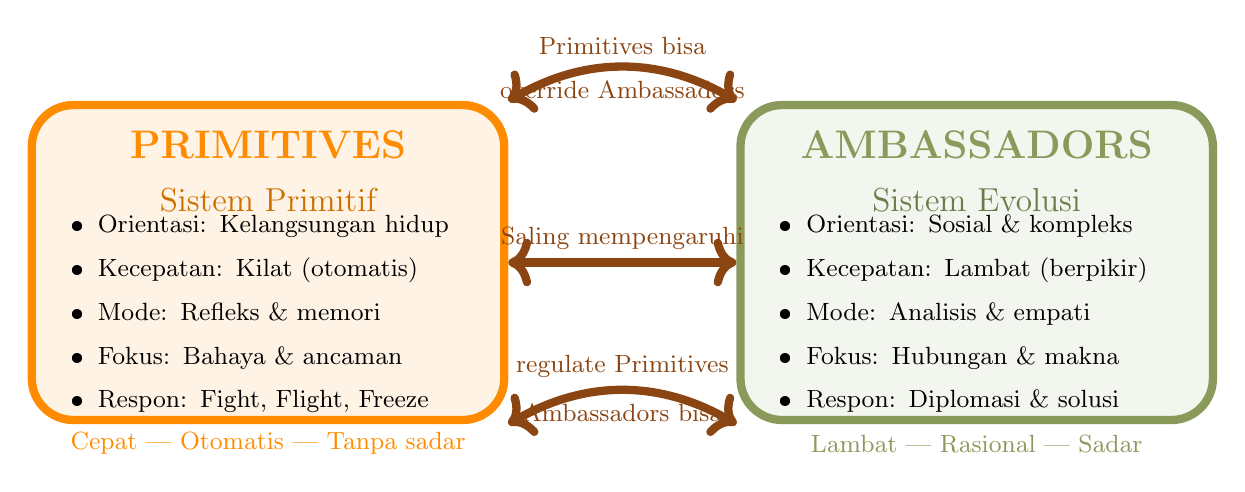
\begin{tikzpicture}[
    box/.style={draw=#1, rounded corners=15pt, fill=#1!10, 
                minimum width=6cm, minimum height=4cm, align=center,
                line width=3pt},
    arrow/.style={<->, line width=3pt, primary}
]
    % Primitives Box
    \node[box=accent] (prim) at (0,0) {};
    \node[font=\Large\bfseries, accent] at (0,1.5) {PRIMITIVES};
    \node[font=\large, accent!80!black] at (0,0.8) {Sistem Primitif};
    \node[align=left, text width=5cm, font=\small] at (0,-0.5) {
        \begin{itemize}[leftmargin=*, itemsep=0.1cm]
            \item Orientasi: Kelangsungan hidup
            \item Kecepatan: Kilat (otomatis)
            \item Mode: Refleks \& memori
            \item Fokus: Bahaya \& ancaman
            \item Respon: Fight, Flight, Freeze
        \end{itemize}
    };
    \node[font=\small\color{accent}] at (0,-2.3) {Cepat | Otomatis | Tanpa sadar};
    
    % Ambassadors Box
    \node[box=sagegreen] (amb) at (9,0) {};
    \node[font=\Large\bfseries, sagegreen] at (9,1.5) {AMBASSADORS};
    \node[font=\large, sagegreen!80!black] at (9,0.8) {Sistem Evolusi};
    \node[align=left, text width=5cm, font=\small] at (9,-0.5) {
        \begin{itemize}[leftmargin=*, itemsep=0.1cm]
            \item Orientasi: Sosial \& kompleks
            \item Kecepatan: Lambat (berpikir)
            \item Mode: Analisis \& empati
            \item Fokus: Hubungan \& makna
            \item Respon: Diplomasi \& solusi
        \end{itemize}
    };
    \node[font=\small\color{sagegreen}] at (9,-2.3) {Lambat | Rasional | Sadar};
    
    % Arrows
    \draw[arrow] (prim.east) -- (amb.west) node[midway, above, font=\small] {Saling mempengaruhi};
    \draw[arrow, bend left=30] (prim.north east) to node[above, font=\small] {Primitives bisa} node[below, font=\small] {override Ambassadors} (amb.north west);
    \draw[arrow, bend right=30] (amb.south west) to node[below, font=\small] {Ambassadors bisa} node[above, font=\small] {regulate Primitives} (prim.south east);
\end{tikzpicture}
\end{center}

\section{Deep Dive: Primitives (Sistem Primitif)}

\subsection{Apa itu Primitives?}

\keyterm{Primitives} adalah bagian otak yang paling tua secara evolusi. Mereka ada untuk satu tujuan: \textbf{membuatmu tetap hidup}.

\begin{praktikbox}[Fungsi Primitives]
\begin{itemize}
    \item \textbf{Survival-focused:} Selalu mencari ancaman
    \item \textbf{Automatic:} Bereaksi tanpa pikir panjang
    \item \textbf{Memory-based:} Menggunakan memori lama untuk menilai situasi sekarang
    \item \textbf{Reflex-driven:} Refleks adalah bosnya
    \item \textbf{Danger-detection:} Selalu waspada
\end{itemize}
\end{praktikbox}

\subsection{Komponen Kunci Primitives}

\begin{center}
\renewcommand{\arraystretch}{1.5}
\begin{tabular}{|>{\raggedright}p{3.5cm}|>{\raggedright}p{5cm}|>{\raggedright\arraybackslash}p{6.5cm}|}
\hline
\rowcolor{accent!20}
\textbf{Struktur} & \textbf{Fungsi} & \textbf{Dalam Hubungan} \\
\hline
\textbf{Amygdala} & Alarm bahaya & Mendeteksi ancaman dalam suara, wajah, atau gerakan pasangan \\
\hline
\textbf{Brain Stem} & Fungsi dasar (napas, detak jantung) & Saat stres, mengontrol respons fisiologis seperti jantung berdebar \\
\hline
\textbf{Cerebellum} & Koordinasi motorik & Gerakan tiba-tiba saat marah atau ketakutan \\
\hline
\textbf{Basal Ganglia} & Kebiasaan dan reward & Membuatmu ``kecanduan'' pasangan melalui dopamine \\
\hline
\textbf{Hippocampus} (bagian) & Memori emosional & Mengingat pengalaman traumatis masa lalu \\
\hline
\end{tabular}
\end{center}

\subsection{Bagaimana Primitives Bekerja dalam Dating?}

Saat kamu melihat seseorang yang menarik:

\begin{enumerate}
    \item \textbf{Far Visual System} (bagian dari primitives) mendeteksi gerakan, bentuk, sinyal atraksi
    \item \textbf{Amygdala} memutuskan: ``Aman atau berbahaya?''
    \item Jika ``aman'', \textbf{Basal Ganglia} rilis dopamine --- sensasi ``suka''
    \item Jika ada red flag tapi \textbf{familiar}, primitives mungkin bilang ``Aman!'' karena familiar = aman untuk otak primitif
\end{enumerate}

\begin{warningbox}[Bahaya Primitives dalam Hubungan]
\begin{itemize}
    \item \textbf{False alarm:} Amygdala bisa melihat ``ancaman'' padahal pasanganmu hanya capek
    \item \textbf{Familiar trap:} Kamu tertarik pada orang yang seperti orang tua yang menyakitimu (karena familiar)
    \item \textbf{Overreaction:} Respon fight/flight yang berlebihan saat konflik kecil
\end{itemize}
\end{warningbox}

\section{Deep Dive: Ambassadors (Sistem Evolusi)}

\subsection{Apa itu Ambassadors?}

\keyterm{Ambassadors} adalah bagian otak yang lebih baru secara evolusi. Mereka adalah ``diplomat'' yang bisa:

\begin{praktikbox}[Fungsi Ambassadors]
\begin{itemize}
    \item \textbf{Nuanced judgment:} Menilai situasi secara kompleks, tidak hitam-putih
    \item \textbf{Empathy:} Merasakan apa yang dirasakan orang lain
    \item \textbf{Delayed gratification:} Menunda kesenangan untuk tujuan jangka panjang
    \item \textbf{Planning:} Merencanakan dan memprediksi
    \item \textbf{Social regulation:} Mengontrol ekspresi sosial agar sesuai norma
\end{itemize}
\end{praktikbox}

\subsection{Komponen Kunci Ambassadors}

\begin{center}
\renewcommand{\arraystretch}{1.5}
\begin{tabular}{|>{\raggedright}p{3.5cm}|>{\raggedright}p{5cm}|>{\raggedright\arraybackslash}p{6.5cm}|}
\hline
\rowcolor{sagegreen!20}
\textbf{Struktur} & \textbf{Fungsi} & \textbf{Dalam Hubungan} \\
\hline
\textbf{Prefrontal Cortex} & Pengambilan keputusan, kontrol impuls & Menahan diri tidak menyakiti pasangan saat marah \\
\hline
\textbf{Anterior Cingulate} & Deteksi error, empati & Menyadari ``Aku salah'' dan memahami perasaan pasangan \\
\hline
\textbf{Orbital Frontal Cortex} & Penilaian sosial, kontrol emosi & Membaca ekspresi wajah pasangan dengan akurat \\
\hline
\textbf{Hippocampus} (utama) & Memori eksplisit, konteks & Mengingat detail tentang pasangan (Love Maps) \\
\hline
\textbf{Insula} & Kesadaran tubuh, intuisi & ``Merasakan'' bahwa sesuatu salah dalam hubungan \\
\hline
\end{tabular}
\end{center}

\section{Konflik Antara Primitives dan Ambassadors}

\subsection{Skenario: Lihat Mantan di Media Sosial}

\begin{center}
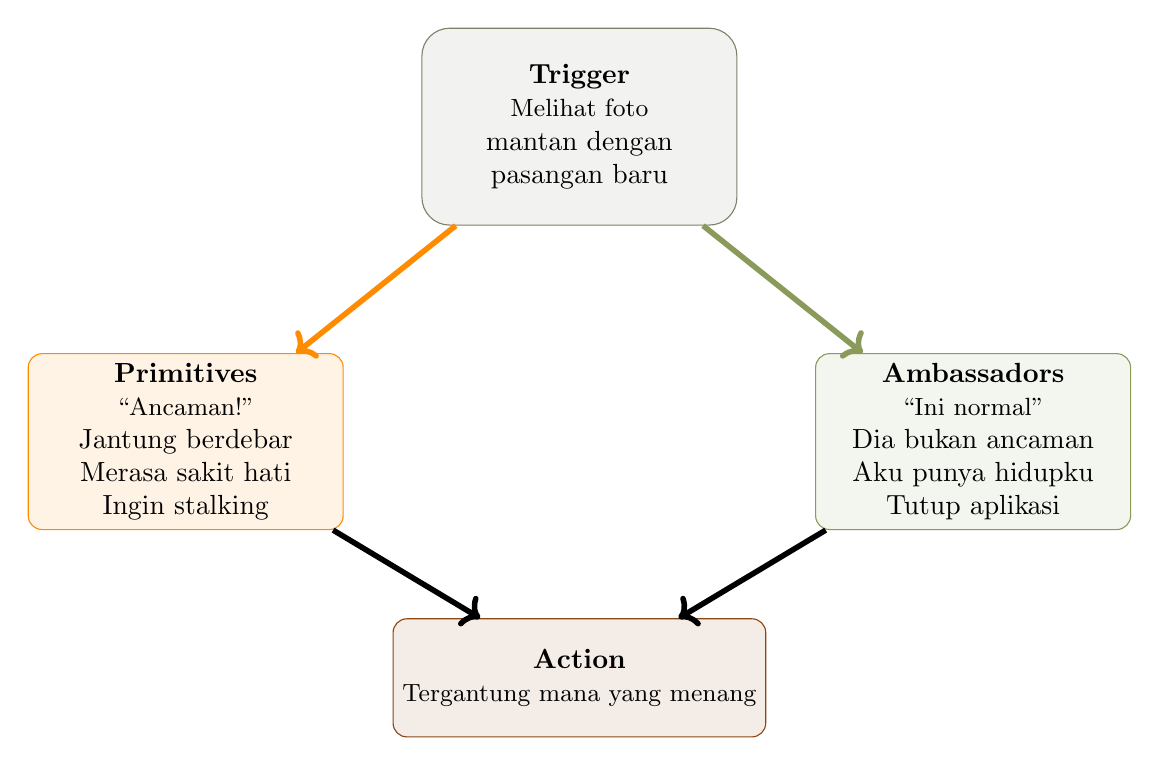
\begin{tikzpicture}[
    scenario/.style={draw=warmgray, rounded corners=10pt, fill=warmgray!10,
                     minimum width=4cm, minimum height=2.5cm, align=center},
    response/.style={draw=#1, rounded corners=5pt, fill=#1!10,
                     minimum width=4cm, minimum height=1.5cm, align=center}
]
    % Trigger
    \node[scenario] (trigger) at (0,0) {\textbf{Trigger}\\\small Melihat foto\\mantan dengan\\pasangan baru};
    
    % Primitives Response
    \node[response=accent] (prim) at (-5,-4) {\textbf{Primitives}\\\small ``Ancaman!''\\Jantung berdebar\\Merasa sakit hati\\Ingin stalking};
    
    % Ambassadors Response
    \node[response=sagegreen] (amb) at (5,-4) {\textbf{Ambassadors}\\\small ``Ini normal''\\Dia bukan ancaman\\Aku punya hidupku\\Tutup aplikasi};
    
    % Final Action
    \node[response=primary] (action) at (0,-7) {\textbf{Action}\\\small Tergantung mana yang menang};
    
    % Arrows
    \draw[->, line width=2pt, accent] (trigger) -- (prim);
    \draw[->, line width=2pt, sagegreen] (trigger) -- (amb);
    \draw[->, line width=2pt] (prim) -- (action);
    \draw[->, line width=2pt] (amb) -- (action);
\end{tikzpicture}
\end{center}

\subsection{Kapan Ambassadors Offline?}

Ambassadors \textbf{tidak berfungsi} saat:
\begin{enumerate}
    \item \textbf{Flooding:} Jantung berdebar $>$100 bpm, darah naik
    \item \textbf{Sleep deprivation:} Kurang tidur
    \item \textbf{Drunk/High:} Terpengaruh zat
    \item \textbf{Extreme hunger:} Sangat lapar
    \item \textbf{Fog of infatuation:} Dopamine tinggi
\end{enumerate}

\begin{tipbox}[Cara Membangunkan Ambassadors]
Saat kamu merasa ``dikuasai'' primitives:
\begin{enumerate}
    \item \textbf{Grounding:} Rasakan kontak kaki dengan lantai
    \item \textbf{Labeling:} Ucapkan ``Ini hanya amydala-ku yang bereaksi''
    \item \textbf{Breathing:} Napas dalam 4-7-8 (tarik 4, tahan 7, hembus 8)
    \item \textbf{Cooling:} Kompres air dingin di wajah (mengaktifkan dive reflex)
    \item \textbf{Time-out:} Beri diri waktu 20 menit untuk turun adrenalin
\end{enumerate}
\end{tipbox}

\section{Fog of Infatuation: Kabut Kegilaan Cinta}

\subsection{Neurochemical Cocktail}

Saat jatuh cinta, otakmu dipenuhi koktail kimia:

\begin{center}
\begin{tikzpicture}[
    chem/.style={draw=#1, line width=2pt, rounded corners=10pt, 
                 fill=#1!10, minimum width=4cm, minimum height=2.5cm, align=center},
    arrow/.style={->, line width=1.5pt}
]
    % Top row
    \node[chem=secondary] (dop) at (0,0) {\textbf{Dopamine}\\\small Pleasure/Reward\\\faArrowUp \ Euforia};
    \node[chem=accent] (nora) at (5,0) {\textbf{Norepinephrine}\\\small Excitement/Focus\\\faArrowUp \ Jantung berdebar};
    \node[chem=warmgray] (sero) at (10,0) {\textbf{Serotonin}\\\small Mood regulation\\\faArrowDown \ Obsesi};
    
    % Bottom row
    \node[chem=softpink] (test) at (2.5,-3.5) {\textbf{Testosterone}\\\small Libido\\Turun (pria), Naik (wanita)};
    \node[chem=sagegreen] (oxy) at (7.5,-3.5) {\textbf{Oxytocin}\\\small Bonding\\\faArrowUp \ Keterikatan};
    
    % Effects
    \node[draw=primary, rounded corners=10pt, fill=primary!10, 
          minimum width=12cm, minimum height=2cm, align=center] (effect) at (5,-6.5) {
        \textbf{Efek Gabungan:} Kurang tidur, kurang makan, obsesi berpikir tentang dia,\\
        mengabaikan red flags, merasa ``ini yang terbaik!''
    };
    
    % Arrows
    \draw[arrow, secondary] (dop) -- (test);
    \draw[arrow, accent] (nora) -- (oxy);
    \draw[arrow, warmgray] (sero) -- (oxy);
    \draw[arrow, softpink] (test) -- (effect);
    \draw[arrow, sagegreen] (oxy) -- (effect);
\end{tikzpicture}
\end{center}

\subsection{Fakta Mengejutkan tentang Serotonin}

\begin{warningbox}[The Serotonin Drop]
\begin{itemize}
    \item Saat jatuh cinta, \textbf{serotonin turun 40\%}
    \item Level yang sama dengan penderita \textbf{OCD} (Obsessive Compulsive Disorder)
    \item Ini sebabnya kamu \textbf{tidak bisa berhenti memikirkan} dia
    \item Ini juga sebabnya kamu \textbf{obsesif} --- cek hp terus, stalking media sosial
\end{itemize}

\textit{``Crazy in love'' bukan hanya metafora --- ini kondisi neurokimia yang nyata!}
\end{warningbox}

\subsection{Durasi Fog of Infatuation}

Kabut ini \textbf{tidak abadi}:
\begin{itemize}
    \item \textbf{3-6 bulan:} Puncak euforia
    \item \textbf{6-12 bulan:} Mulai turun
    \item \textbf{12-24 bulan:} Kembali ke normal
    \item \textbf{Setelah itu:} Attachment (oxytocin/vasopressin) mengambil alih
\end{itemize}

\begin{insightbox}
\textbf{Implikasi:} Jangan ambil keputusan besar (menikah, pindah bareng, investasi besar) dalam 12-18 bulan pertama hubungan. Tunggu sampai fog hilang untuk melihat realitas dengan jelas.
\end{insightbox}

\section{Visual System: Far vs Near}

Otak punya dua jalur visual yang berbeda:

\begin{center}
\renewcommand{\arraystretch}{1.6}
\begin{tabular}{|>{\raggedright}p{3cm}|>{\raggedright}p{5.5cm}|>{\raggedright\arraybackslash}p{5.5cm}|}
\hline
\rowcolor{primary!20}
\textbf{Aspek} & \textbf{Far Visual System} & \textbf{Near Visual System} \\
\hline
\textbf{Alias} & Dorsal stream (``where/how'') & Ventral stream (``what'') \\
\hline
\textbf{Fungsi utama} & Deteksi gerakan, lokasi, arah & Detail wajah, ekspresi, identifikasi \\
\hline
\textbf{Resolusi} & Rendah (blur) & Tinggi (tajam) \\
\hline
\textbf{Hubungan dengan} & \textbf{Primitives} & \textbf{Ambassadors} \\
\hline
\textbf{Jarak optimal} & $>$ 1 meter & $<$ 1 meter \\
\hline
\textbf{Deteksi} & Bahaya, atraksi kasar & Emosi, niat, kebohongan \\
\hline
\textbf{Dalam dating} & ``Orang itu hot!'' (dari kejauhan) & ``Dia bohong'' (dari dekat) \\
\hline
\end{tabular}
\end{center}

\subsection{Mengapa ``Cinta Pada Pandangan Pertama'' Menipu}

Far Visual System:
\begin{itemize}
    \item Melihat gerakan pinggul, cara berjalan, siluet
    \item \textbf{Mengaktifkan Primitives}
    \item Memberi sinyal ``Ini orang yang menarik''
    \item Tapi \textbf{tidak bisa menilai} karakter, kejujuran, kompatibilitas
\end{itemize}

\begin{tipbox}[Gunakan Near Visual System dengan Benar]
Untuk benar-benar mengenal seseorang:
\begin{itemize}
    \item Duduk \textbf{berhadapan} dalam jarak $<$ 1 meter
    \item Pastikan \textbf{PENCAYAAN CUKUP} (jangan tempat gelap)
    \item Lihat ke \textbf{mata} --- pupil, micro-expression
    \item Perhatikan \textbf{asimetri wajah} --- alkohol/membuat wajah terlihat lebih simetris/simetris = menarik
    \item Lakukan ini \textbf{berulang kali} dalam berbagai situasi
\end{itemize}
\end{tipbox}

\section{Sistem Saraf dalam Relasi: Polyvagal Theory}

Stephen Porges mengembangkan teori tentang tiga mode respons saraf kita dalam interaksi sosial.

\begin{center}
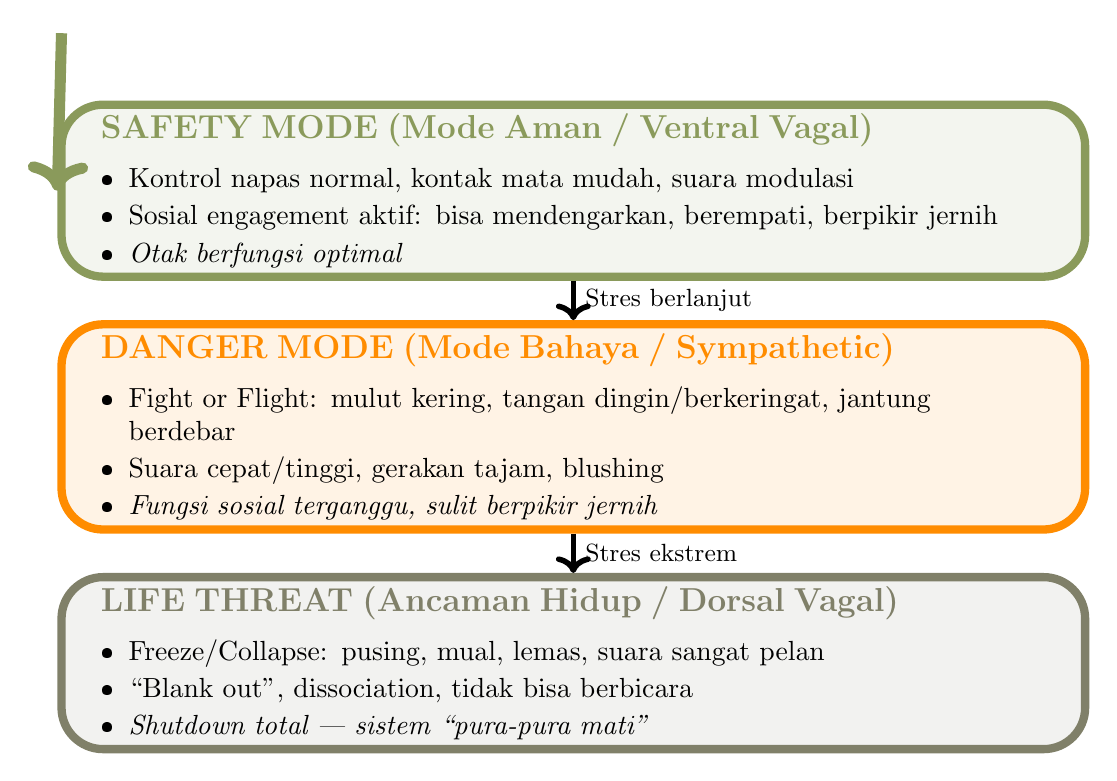
\begin{tikzpicture}[
    mode/.style={draw=#1, line width=3pt, rounded corners=15pt,
                 fill=#1!10, minimum width=13cm, minimum height=2cm,
                 align=left, text width=12cm}
]
    \node[mode=sagegreen] (safe) at (0,4) {
        \textbf{\large \textcolor{sagegreen}{SAFETY MODE (Mode Aman / Ventral Vagal)}}\\[0.2cm]
        \begin{itemize}[leftmargin=*, itemsep=0.05cm]
            \item Kontrol napas normal, kontak mata mudah, suara modulasi
            \item Sosial engagement aktif: bisa mendengarkan, berempati, berpikir jernih
            \item \textit{Otak berfungsi optimal}
        \end{itemize}
    };
    
    \node[mode=accent] (danger) at (0,1) {
        \textbf{\large \textcolor{accent}{DANGER MODE (Mode Bahaya / Sympathetic)}}\\[0.2cm]
        \begin{itemize}[leftmargin=*, itemsep=0.05cm]
            \item Fight or Flight: mulut kering, tangan dingin/berkeringat, jantung berdebar
            \item Suara cepat/tinggi, gerakan tajam, blushing
            \item \textit{Fungsi sosial terganggu, sulit berpikir jernih}
        \end{itemize}
    };
    
    \node[mode=warmgray] (threat) at (0,-2) {
        \textbf{\large \textcolor{warmgray}{LIFE THREAT (Ancaman Hidup / Dorsal Vagal)}}\\[0.2cm]
        \begin{itemize}[leftmargin=*, itemsep=0.05cm]
            \item Freeze/Collapse: pusing, mual, lemas, suara sangat pelan
            \item ``Blank out'', dissociation, tidak bisa berbicara
            \item \textit{Shutdown total --- sistem ``pura-pura mati''}
        \end{itemize}
    };
    
    \draw[->, line width=4pt, sagegreen] (-6.5,6) -- (safe.west);
    \draw[->, line width=2pt] (safe.south) -- (danger.north) node[midway, right, font=\small] {Stres berlanjut};
    \draw[->, line width=2pt] (danger.south) -- (threat.north) node[midway, right, font=\small] {Stres ekstrem};
\end{tikzpicture}
\end{center}

\subsection{Co-Regulation: Menenangkan Satu Sama Lain}

\begin{insightbox}
Manusia adalah satu-satunya mamalia yang \textbf{tidak bisa} menenangkan diri sendiri dengan efektif. Kita butuh \keyterm{co-regulation} --- saling menenangkan dengan interaksi sosial.
\end{insightbox}

\textbf{Tanda-tanda butuh co-regulation:}
\begin{itemize}
    \item Jantung berdebar
    \item Napas pendek/cepat
    \item Otot tegang
    \item Pikiran berkecamuk
    \item Ingin menjauh atau menyerang
\end{itemize}

\textbf{Cara co-regulate dengan pasangan:}
\begin{enumerate}
    \item \textbf{Kontak fisik:} Pegang tangan, peluk (jika nyaman)
    \item \textbf{Kontak mata lembut:} Soft eye contact
    \item \textbf{Suara rendah dan lambat:} ``Aku di sini'', ``Kita aman''
    \item \textbf{Breathing together:} Napas bersamaan
    \item \textbf{Validation:} ``Aku mengerti kamu stres''
\end{enumerate}

\section{Familiarity Effect: Jebakan yang Dikenal}

Otak tertarik pada yang \textbf{familiar} --- tapi familiar $\neq$ sehat.

\subsection{Mere Exposure Effect}

Semakin sering kamu melihat sesuatu, semakin kamu menyukainya.

\begin{praktikbox}[Efek Familiar dalam Hubungan]
\textbf{Familiar yang Sehat:}
\begin{itemize}
    \item Orang yang menghargai hubungan dan terbuka
    \item Pola komunikasi jujur dan langsung
    \item Rasa aman tanpa drama
    \item Konflik yang diselesaikan dengan baik
\end{itemize}

\textbf{Familiar yang Tidak Sehat:}
\begin{itemize}
    \item Orang seperti orang tua yang tidak stabil
    \item Drama, chaos, roller-coaster emosi
    \item Sikap dingin/menghindar (jika kamu Island)
    \item Sikap clingy/cemas (jika kamu Wave)
\end{itemize}
\end{praktikbox}

\begin{warningbox}[Trauma Bonding]
Jika kamu dibesarkan dalam lingkungan yang tidak stabil, kamu mungkin merasa ``nyaman'' dengan pasangan yang juga tidak stabil. Ini disebut \textbf{trauma bonding} --- hubungan berbasis trauma yang sama.

\textbf{Tanda-tanda:}
\begin{itemize}
    \item Merasa ``hidup'' hanya saat ada drama
    \item Pasangan yang baik-baik saja terasa membosankan
    \item Selalu tertarik pada orang yang ``perlu diselamatkan''
    \item Pola hubungan berulang yang tidak memuaskan
\end{itemize}
\end{warningbox}

\section{Action Steps: Praktik Mingguan}

\begin{exercisebox}[Program 7 Hari: Mengenali Wiring-mu]

\textbf{Hari 1-2: Mindful Breathing (5 menit)}
\begin{itemize}
    \item Duduk nyaman, punggung lurus
    \item Tarik napas 4 detik $\rightarrow$ Tahan 4 detik $\rightarrow$ Hembusk 6 detik
    \item Fokus hanya pada napas
    \item Jika pikiran melayang, kembalikan tanpa menghakimi
\end{itemize}

\textbf{Hari 3-4: Body Scan saat Dating/Berpasangan}
\begin{itemize}
    \item Sebelum bertemu pasangan, tutup mata
    \item Scan dari kepala ke kaki: di mana ketegangan?
    \item Catat di jurnal: ``Saat akan bertemu dia, aku merasa...''
\end{itemize}

\textbf{Hari 5-6: Deteksi Fog}
\begin{itemize}
    \item Apakah jantungku berdebar kencang memikirkan dia?
    \item Apakah aku sulit tidur/makan karena memikirkannya?
    \item Apakah aku mengabaikan kekurangan yang jelas?
    \item Jika ya, tulis: ``Ini hanya kimia. Aku perlu waktu untuk melihat dengan jelas.''
\end{itemize}

\textbf{Hari 7: Reflection}
\begin{itemize}
    \item Review jurnal minggu ini
    \item Identifikasi: Kapan Primitives-mu bereaksi berlebihan?
    \item Kapan Ambassadors-mu berhasil mengontrol?
    \item Apa strategi yang paling efektif untukmu?
\end{itemize}
\end{exercisebox}

\begin{tipbox}[Quick Reference Card]
\textbf{Saat kamu merasa ``dikuasai'' emosi:}
\begin{enumerate}
    \item \textbf{STOP} --- jangan reaksi dulu
    \item \textbf{BREATHE} --- 3 napas dalam
    \item \textbf{LABEL} --- ``Ini amydala-ku''
    \item \textbf{GROUND} --- Rasakan kaki di lantai
    \item \textbf{WAIT} --- 20 menit sebelum merespons
\end{enumerate}
\end{tipbox}

\chapter{Love Maps: Peta Cinta yang Detail}

\begin{insightbox}
\textit{``Untuk mencintai seseorang, kamu harus mengenalnya. Dan mengenal itu bukan sekadar tahu makanan favoritnya --- tapi tahu luka-lukanya, mimpi-mimpinya, dan bagaimana cara pandangnya tentang dunia.''}
\end{insightbox}

\section{Apa itu Love Maps?}

\keyterm{Love Maps} adalah istilah Dr. John Gottman untuk menggambarkan bagian otak tempat kita menyimpan semua informasi relevan tentang kehidupan pasangan. Semakin detail peta ini, semakin kuat fondasi hubungan.

\begin{praktikbox}[Definisi Love Maps]
\textbf{Love Maps} adalah:
\begin{itemize}
    \item Pengetahuan mendalam tentang dunia internal pasangan
    \item Memori tentang peristiwa penting dalam hidupnya
    \item Pemahaman tentang tekanan, kekhawatiran, dan harapannya
    \item Kesadaran akan perubahan dan evolusi dalam dirinya
    \item ``Cognitive room'' yang kamu buat untuk hubungan ini
\end{itemize}
\end{praktikbox}

\subsection{Kenapa Love Maps Penting?}

\begin{center}
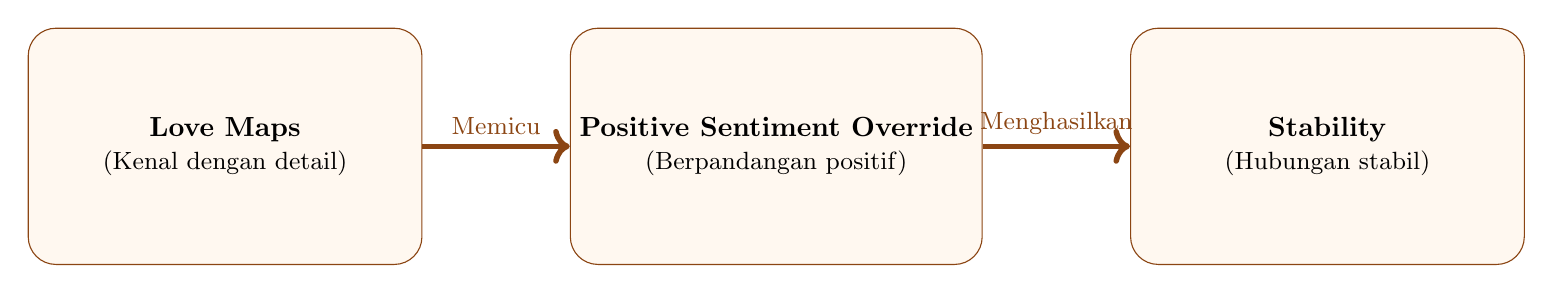
\begin{tikzpicture}[
    box/.style={draw=primary, rounded corners=10pt, fill=lightbg,
                minimum width=5cm, minimum height=3cm, align=center},
    arrow/.style={->, line width=2pt, primary}
]
    \node[box] (lm) at (0,0) {\textbf{Love Maps}\\\small (Kenal dengan detail)};
    \node[box] (p) at (7,0) {\textbf{Positive Sentiment Override}\\\small (Berpandangan positif)};
    \node[box] (s) at (14,0) {\textbf{Stability}\\\small (Hubungan stabil)};
    
    \draw[arrow] (lm) -- (p) node[midway, above, font=\small] {Memicu};
    \draw[arrow] (p) -- (s) node[midway, above, font=\small] {Menghasilkan};
\end{tikzpicture}
\end{center}

\textbf{Studi Gottman menemukan:}
\begin{itemize}
    \item Pasangan dengan Love Maps yang detail memiliki hubungan yang lebih kuat setelah lahiran anak pertama (waktu 67\% pasangan mengalami penurunan kepuasan)
    \item Love Maps \textbf{melindungi} hubungan saat stres tinggi
    \item Tanpa Love Maps, pasangan mudah ``tenggelam'' dalam perubahan hidup
\end{itemize}

\section{Komponen Love Maps yang Lengkap}

\subsection{Level 1: Fakta Dasar (Harus Tahu)}

\begin{center}
\renewcommand{\arraystretch}{1.4}
\begin{tabular}{|>{\raggedright}p{5cm}|>{\raggedright\arraybackslash}p{10cm}|}
\hline
\rowcolor{primary!20}
\textbf{Kategori} & \textbf{Contoh Pertanyaan} \\
\hline
\textbf{Keseharian} & 
\begin{itemize}[leftmargin=*, itemsep=0.05cm]
    \item Apa yang dia lakukan hari ini?
    \item Siapa teman terdekatnya?
    \item Apa stres yang sedang dihadapinya?
\end{itemize} \\
\hline
\textbf{Preferensi} & 
\begin{itemize}[leftmargin=*, itemsep=0.05cm]
    \item Makanan favorit?
    \item Musik/ film/ buku favorit?
    \item Cara menghabiskan akhir pekan ideal?
\end{itemize} \\
\hline
\textbf{Keluarga} & 
\begin{itemize}[leftmargin=*, itemsep=0.05cm]
    \item Bagaimana hubungannya dengan ayah/ibu?
    \item Siapa kerabat favorit dan yang paling tidak disukai?
    \item Tradisi keluarga apa yang penting baginya?
\end{itemize} \\
\hline
\textbf{Karir} & 
\begin{itemize}[leftmargin=*, itemsep=0.05cm]
    \item Apa aspirasi karirnya?
    \item Siapa rekan kerja yang menyebalkan?
    \item Apa proyek penting saat ini?
\end{itemize} \\
\hline
\end{tabular}
\end{center}

\subsection{Level 2: Dunia Emosional (Perlu Usaha)}

\begin{praktikbox}[Mengenal Dunia Emosional]
\begin{itemize}
    \item \textbf{Fears:} Apa ketakutan terbesarnya? (Fisik? Emosional? Eksistensial?)
    \item \textbf{Dreams:} Mimpi apa yang belum tercapai?
    \item \textbf{Regrets:} Penyesalan apa yang masih membekas?
    \item \textbf{Proud moments:} Momen apa yang paling dibanggakan?
    \item \textbf{Vulnerabilities:} Luka dari masa kecil yang masih ada?
\end{itemize}
\end{praktikbox}

\subsection{Level 3: Filosofi Hidup (Butuh Waktu Lama)}

\begin{itemize}
    \item \textbf{Meaning of life:} Apa makna hidup baginya?
    \item \textbf{Values:} Nilai apa yang paling penting? (Keluarga? Karir? Kebebasan?)
    \item \textbf{Spirituality:} Pandangan spiritual/religius?
    \item \textbf{Legacy:} Apa warisan yang ingin ditinggalkan?
    \item \textbf{Worldview:} Bagaimana dia melihat dunia? (Optimis? Pesimis? Pragmatis?)
\end{itemize}

\section{Love Maps Questionnaire}

\begin{exercisebox}[Love Maps Assessment]
\textbf{Petunjuk:} Jawab pertanyaan berikut tentang pasanganmu. Lihat seberapa banyak yang bisa kamu jawab dengan tepat.

\subsection*{Fakta Dasar (1 poin per jawaban benar)}
\begin{enumerate}
    \item Sebutkan dua teman terdekat pasanganmu.
    \item Apa stres yang sedang dihadapi pasanganmu akhir-akhir ini?
    \item Sebutkan nama-nama orang yang baru-baru ini menyebalkan pasanganmu di tempat kerja.
    \item Apa mimpi yang belum tercapai dari pasanganmu?
    \item Apa keyakinan agama/kepercayaan pasanganmu?
    \item Apa filosofi hidup pasanganmu dalam satu kalimat?
    \item Siapa kerabat yang paling tidak disukai pasanganmu?
    \item Apa musik/grup favorit pasanganmu?
    \item Sebutkan tiga film favorit pasanganmu.
    \item Apakah pasanganmu tahu stres yang sedang kamu hadapi?
\end{enumerate}

\subsection*{Memori Bersama (1 poin per jawaban benar)}
\begin{enumerate}
    \item[11.] Sebutkan tiga momen paling spesial dalam hidup pasanganmu.
    \item[12.] Apa peristiwa paling stresful yang dialami pasanganmu saat kecil?
    \item[13.] Sebutkan aspirasi dan harapan besar dalam hidup pasanganmu.
    \item[14.] Apa kekhawatiran utama pasanganmu saat ini?
    \item[15.] Apakah pasanganmu tahu siapa teman-temanmu?
    \item[16.] Apa yang akan dilakukan pasanganmu jika tiba-tiba memenangkan lotere?
    \item[17.] Ceritakan kesan pertamamu tentang pasanganmu secara detail.
    \item[18.] Seberapa sering kamu bertanya kepada pasangan tentang dunianya saat ini?
    \item[19.] Apakah pasanganmu merasa kamu mengenalnya dengan baik?
    \item[20.] Apakah pasanganmu tahu harapan dan aspirasimu?
\end{enumerate}

\textbf{Scoring:}
\begin{itemize}
    \item \textbf{16-20 poin:} Love Maps-mu sangat detail. Hubunganmu punya fondasi yang kuat.
    \item \textbf{10-15 poin:} Cukup baik, tapi ada ruang untuk mendalami.
    \item \textbf{Kurang dari 10:} Love Maps-mu perlu diperbarui segera. Risiko hubungan terancam.
\end{itemize}
\end{exercisebox}

\section{Game: Love Maps 20 Questions}

\begin{exercisebox}[Cara Bermain]
\textbf{Waktu:} 30-45 menit\\
\textbf{Tempat:} Tempat nyaman tanpa gangguan\\
\textbf{Alat:} Kertas dan pena

\textbf{Langkah:}
\begin{enumerate}
    \item Masing-masing tentukan 20 angka acak antara 1-60
    \item Bergantian tanyakan pertanyaan sesuai nomor
    \item Jika jawaban benar, penanya dapat poin sesuai nilai pertanyaan
    \item Diskusikan jawabannya --- ini bukan sekadar game, tapi kesempatan belajar
\end{enumerate}
\end{exercisebox}

\subsection{Daftar Pertanyaan Love Maps}

\begin{center}
\renewcommand{\arraystretch}{1.3}
\begin{tabular}{|c|l|c|}
\hline
\rowcolor{primary!20}
\textbf{No} & \textbf{Pertanyaan} & \textbf{Poin} \\
\hline
1 & Sebutkan dua teman terdekatku & 2 \\
\hline
2 & Apa grup musik/komposer/alat musik favoritku? & 2 \\
\hline
3 & Apa yang kupakai saat pertama kali kita bertemu? & 2 \\
\hline
4 & Sebutkan satu hobi yang kumiliki & 3 \\
\hline
5 & Di mana aku lahir? & 1 \\
\hline
6 & Apa stres yang kuhadapi saat ini? & 4 \\
\hline
7 & Deskripsikan detail apa yang kulakukan hari ini/kemarin & 4 \\
\hline
8 & Kapan ulang tahunku? & 1 \\
\hline
9 & Kapan tanggal anniversary kita? & 1 \\
\hline
10 & Siapa kerabat favoritku? & 2 \\
\hline
11 & Apa mimpi terbesar yang belum tercapai? & 5 \\
\hline
12 & Website favoritku? & 2 \\
\hline
13 & Apa satu ketakutan atau skenario bencana terbesarku? & 3 \\
\hline
14 & Jam berapa waktu favoritku untuk bercinta? & 3 \\
\hline
15 & Apa yang membuatku merasa paling kompeten? & 4 \\
\hline
16 & Apa yang membangkitkan gairahku secara seksual? & 3 \\
\hline
17 & Apa makanan favoritku? & 2 \\
\hline
18 & Bagaimana cara favoritku menghabiskan malam? & 2 \\
\hline
19 & Apa warna favoritku? & 1 \\
\hline
20 & Perbaikan diri apa yang ingin kulakukan dalam hidup? & 4 \\
\hline
21 & Hadiah seperti apa yang paling kusukai? & 2 \\
\hline
22 & Apa salah satu pengalaman masa kecil terbaikku? & 2 \\
\hline
23 & Liburan mana yang paling kuingat? & 2 \\
\hline
24 & Apa cara favoritku untuk bersantai? & 4 \\
\hline
25 & Siapa sumber dukungan terbesarku (selain kamu)? & 3 \\
\hline
26 & Apa olahraga favoritku? & 2 \\
\hline
27 & Apa yang paling kusukai lakukan saat libur? & 2 \\
\hline
28 & Apa aktivitas akhir pekan favoritku? & 2 \\
\hline
29 & Di mana tempat liburan impianku? & 3 \\
\hline
30 & Apa film favoritku? & 2 \\
\hline
\end{tabular}
\end{center}

\textit{(Lanjutkan untuk nomor 31-60 dengan pola serupa --- pertanyaan tentang masa depan, pengalaman traumatis, filosofi hidup, dll.)}

\section{Open-Ended Questions untuk Memperdalam}

\begin{tipbox}[Cara Bertanya yang Membuka]
Gunakan pertanyaan \textbf{open-ended} (tidak bisa dijawab ya/tidak) untuk menggali lebih dalam:

\begin{enumerate}
    \item ``Bagaimana kamu ingin hidupmu tiga tahun dari sekarang?''
    \item ``Apa pendapatmu tentang rumah fisik kita? Mau ada perubahan?''
    \item ``Bagaimana perbandingan dirimu sebagai orang tua dengan orang tuamu sendiri?''
    \item ``Jika kamu bisa mengubah satu hal dalam masa lalu, apa itu?''
    \item ``Apa yang paling kamu khawatirkan tentang masa depan?''
    \item ``Siapa yang kamu anggap sahabat atau sekutu terdekat? Daftarnya berubah?''
    \item ``Apa kualitas yang paling kamu hargai pada teman saat ini?''
    \item ``Jika kamu bisa memiliki tiga skill baru secara instan, apa itu?''
    \item ``Apa yang paling kamu sesali dan banggakan dari tahun lalu?''
    \item ``Apa petualangan yang ingin kamu jalani sekarang?''
\end{enumerate}
\end{tipbox}

\section{Latihan Mendalam: ``Who Am I?''}

\begin{exercisebox}[Latihan Self-Exploration]
\textbf{Waktu:} 2-3 jam (bisa dipecah beberapa sesi)\\
\textbf{Instruksi:} Jawab pertanyaan berikut dalam jurnal pribadi, lalu tukar dan diskusikan dengan pasangan.

\subsection*{1. Triumphs and Strivings (Prestasi dan Perjuangan)}
\begin{enumerate}
    \item Apa yang terjadi dalam hidupmu yang membuatmu bangga?
    \item Bagaimana kesuksesan ini membentuk hidup dan cara pandangmu?
    \item Seberapa besar peran ``rasa bangga'' dalam hidupmu?
    \item Bagaimana orang tuamu menunjukkan kebanggaan padamu?
\end{enumerate}

\subsection*{2. Injuries and Healing (Luka dan Penyembuhan)}
\begin{enumerate}
    \item Peristiwa sulit atau periode apa yang pernah kamu lalui?
    \item Bagaimana kamu bertahan dari trauma tersebut?
    \item Efek jangka panjang apa yang masih ada?
    \item Bagaimana cara kamu melindungi diri agar tidak terluka lagi?
\end{enumerate}

\subsection*{3. My Emotional World (Dunia Emosional)}
\begin{enumerate}
    \item Bagaimana keluargamu mengekspresikan: marah, sedih, takut, kasih sayang?
    \item Apa filosofimu tentang mengekspresikan perasaan?
    \item Perasaan mana yang sulit bagimu ekspresikan atau dengar?
\end{enumerate}

\subsection*{4. My Mission and Legacy (Misi dan Warisan)}
\begin{enumerate}
    \item Bayangkan epitaph di batu nisanmu. Apa yang ingin tertulis?
    \item Tulis obituary-mu sendiri. Bagaimana orang mengenangmu?
    \item Apa tujuan hidupmu? Perjuangan besar apa yang sedang dijalan?
    \item Warisan apa yang ingin kamu tinggalkan?
\end{enumerate}
\end{exercisebox}

\section{Memperbarui Love Maps Secara Rutin}

\begin{insightbox}
\textbf{Key Insight:} Love Maps bukan ``set it and forget it''. Orang berubah setiap hari. Love Maps yang tidak diperbarui akan \textbf{kadaluarsa}.
\end{insightbox}

\subsection{Ritual Pembaruan}

\begin{enumerate}
    \item \textbf{Daily:} ``Gimana harimu?'' yang benar-benar didengar
    \item \textbf{Weekly:} 20 menit talking about stresses outside marriage
    \item \textbf{Monthly:} Deep conversation tentang hopes, fears, dreams
    \item \textbf{Yearly:} Review dan update Love Maps questionnaire
\end{enumerate}

\subsection{Tanda Love Maps Perlu Diperbarui}

\begin{warningbox}[Warning Signs]
\begin{itemize}
    \item Kamu bingung kenapa pasanganmu marah/sedih
    \item Kamu terkejut dengan keputusan atau perubahan pasangan
    \item Kamu merasa ``seperti hidup dengan orang asing''
    \item Kamu mengasumsikan pasanganmu ``tetap sama'' seperti dulu
    \item Kamu lebih tahu tentang teman kerja daripada pasanganmu
\end{itemize}
\end{warningbox}

\section{Action Steps}

\begin{exercisebox}[To-Do List Minggu Ini]
\textbf{1. Kerjakan Love Maps Questionnaire} (30 menit)
\begin{itemize}
    \item Jawab sendiri dulu
    \item Bandingkan dengan pasangan
    \item Catat area yang perlu diperdalam
\end{itemize}

\textbf{2. Mainkan Love Maps 20 Questions} (45 menit)
\begin{itemize}
    \item Jadikan malam ini ``game night''
    \item Fokus pada kesenangan dan belajar, bukan kompetisi
\end{itemize}

\textbf{3. Mulai Ritual Daily Check-in}
\begin{itemize}
    \item Setiap hari, 10-15 menit tanpa distraksi
    \item Tanya: ``Gimana harimu? Ada apa?''
    \item Dengarkan dengan penuh perhatian
\end{itemize}

\textbf{4. Jadwalkan Deep Conversation}
\begin{itemize}
    \item Blokir waktu 2-3 jam akhir pekan ini
    \item Kerjakan latihan ``Who Am I?''
    \item Bersiaplah untuk vulnerability
\end{itemize}
\end{exercisebox}

\chapter{Turn Toward: Menghadap ke Pasangan}

\begin{insightbox}
\textit{``Romansa sejati tidak terjadi di Bali atau Paris. Romansa terjadi di supermarket saat dia bertanya 'Apakah mentega kita habis?' dan kamu menjawab 'Aku cek dulu ya' daripada mengabaikannya.''}
\end{insightbox}

\section{Apa itu ``Turning Toward''?}

\keyterm{Turning Toward} adalah kecenderungan untuk merespons usaha pasangan untuk mendapatkan perhatian, kasih sayang, humor, atau dukungan.

\begin{praktikbox}[Definisi Turning Toward]
\textbf{Turning Toward berarti:}
\begin{itemize}
    \item Menanggapi ``bids'' (ajakan koneksi) dari pasangan
    \item Memberikan perhatian meski sedang sibuk
    \item Menunjukkan bahwa ``kamu penting bagiku''
    \item Membangun \keyterm{Emotional Bank Account} (Tabungan Emosional)
\end{itemize}

\textbf{Contoh sederhana:}
\begin{itemize}
    \item Pasangan: ``Lihat kapal itu besar!''
    \item Turn Toward: ``Wah iya, mirip kapal layar yang kita lihat waktu itu ya?''
    \item Turn Away: (tidak mendengar, terus main HP)
    \item Turn Against: ``Iya, terus? Kenapa?''
\end{itemize}
\end{praktikbox}

\section{Jenis-jenis Bids (Ajakan Koneksi)}

\begin{center}
\renewcommand{\arraystretch}{1.5}
\begin{tabular}{|>{\raggedright}p{3cm}|>{\raggedright}p{5cm}|>{\raggedright\arraybackslash}p{7cm}|}
\hline
\rowcolor{primary!20}
\textbf{Jenis Bid} & \textbf{Contoh} & \textbf{Cara Menanggapi} \\
\hline
\textbf{Attention} & ``Lihat burung itu!'' & Berhenti sejenak, lihat, komentar \\
\hline
\textbf{Affection} & Memegang tangan saat jalan & Sambut, pegang balik, tersenyum \\
\hline
\textbf{Humor} & ``Aku kayak orang gila ya hari ini'' & Tertawa, lempar jokes balik \\
\hline
\textbf{Support} & ``Hari ini berat banget di kantor'' & Dengarkan, validasi, tanya ``Mau cerita?'' \\
\hline
\textbf{Help} & ``Bisa tolong ambilkan air?'' & Bantu dengan sukarela, tanpa komplain \\
\hline
\textbf{Interest} & ``Kamu tadi ngapain?'' & Ceritakan dengan detail, ajak ngobrol \\
\hline
\end{tabular}
\end{center}

\section{Data Gottman yang Mengejutkan}

\begin{warningbox}[Statistik Penting]
Dalam penelitian 6 tahun terhadap pasangan baru menikah:
\begin{itemize}
    \item Pasangan yang \textbf{bertahan}: merespons bids \textbf{86\%} dari waktu
    \item Pasangan yang \textbf{bercerai}: merespons bids hanya \textbf{33\%} dari waktu
    \item \textbf{Selisih hanya 6 respons dari 10 bids} membedakan hubungan yang berhasil vs gagal!
\end{itemize}

\textit{Perbedaan kecil dalam keseharian = Perbedaan besar dalam hasil jangka panjang}
\end{warningbox}

\section{Tiga Respon terhadap Bids}

\begin{center}
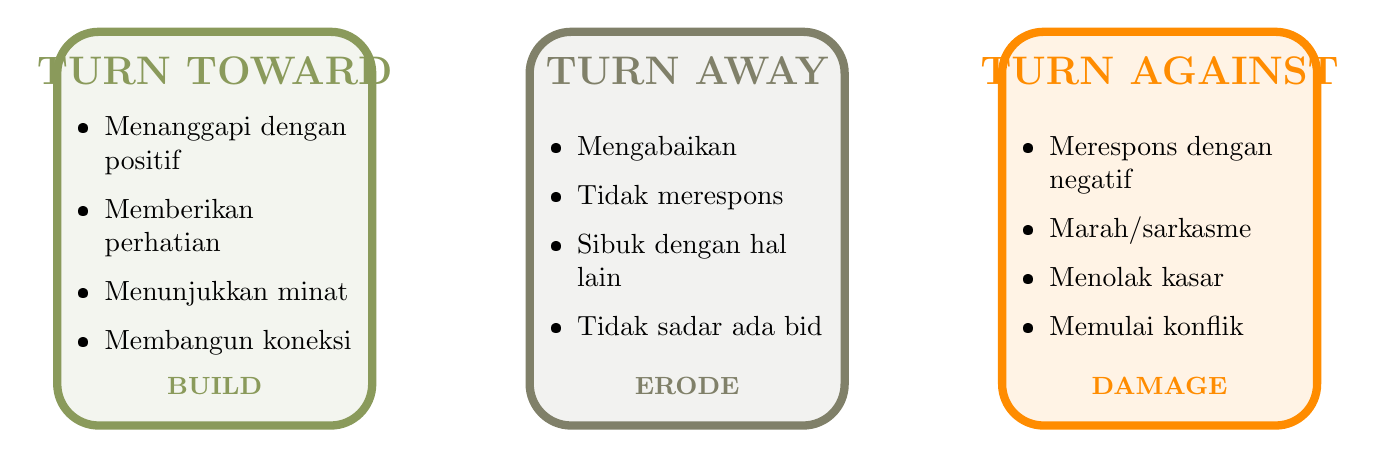
\begin{tikzpicture}[
    response/.style={draw=#1, line width=3pt, rounded corners=15pt,
                     fill=#1!10, minimum width=4cm, minimum height=5cm, align=center},
    title/.style={font=\Large\bfseries}
]
    % Turn Toward
    \node[response=sagegreen] (toward) at (0,0) {};
    \node[title, sagegreen] at (0,2) {TURN TOWARD};
    \node[align=left, text width=3.5cm] at (0,0) {
        \begin{itemize}[leftmargin=*, itemsep=0.2cm]
            \item Menanggapi dengan positif
            \item Memberikan perhatian
            \item Menunjukkan minat
            \item Membangun koneksi
        \end{itemize}
    };
    \node[font=\small\bfseries, sagegreen] at (0,-2) {BUILD};
    
    % Turn Away
    \node[response=warmgray] (away) at (6,0) {};
    \node[title, warmgray] at (6,2) {TURN AWAY};
    \node[align=left, text width=3.5cm] at (6,0) {
        \begin{itemize}[leftmargin=*, itemsep=0.2cm]
            \item Mengabaikan
            \item Tidak merespons
            \item Sibuk dengan hal lain
            \item Tidak sadar ada bid
        \end{itemize}
    };
    \node[font=\small\bfseries, warmgray] at (6,-2) {ERODE};
    
    % Turn Against
    \node[response=accent] (against) at (12,0) {};
    \node[title, accent] at (12,2) {TURN AGAINST};
    \node[align=left, text width=3.5cm] at (12,0) {
        \begin{itemize}[leftmargin=*, itemsep=0.2cm]
            \item Merespons dengan negatif
            \item Marah/sarkasme
            \item Menolak kasar
            \item Memulai konflik
        \end{itemize}
    };
    \node[font=\small\bfseries, accent] at (12,-2) {DAMAGE};
\end{tikzpicture}
\end{center}

\section{Emotional Bank Account}

\begin{praktikbox}[Konsep Tabungan Emosional]
Setiap kali kamu \textbf{Turn Toward}, kamu menyetor ke ``Tabungan Emosional''. Setiap kali \textbf{Turn Away}, kamu menarik.

\textbf{Manfaat saldo tinggi:}
\begin{itemize}
    \item Pasangan lebih toleran terhadap kesalahan kecil
    \item Konflik tidak meledak menjadi besar
    \item Rasa percaya lebih kuat
    \item Hubungan tahan terhadap stres eksternal
\end{itemize}

\textbf{Risiko saldo rendah:}
\begin{itemize}
    \item Setiap kesalahan terasa besar
    \item Konflik kecil jadi besar
    \item Negativity Override (cenderung melihat negatif)
    \item Mudah putus asa saat ada masalah
\end{itemize}
\end{praktikbox}

\subsection{50 Activities yang Membangun Tabungan}

\begin{center}
\small
\renewcommand{\arraystretch}{1.2}
\begin{tabular}{|c|l|c|l|}
\hline
\rowcolor{primary!20}
\textbf{No} & \textbf{Aktivitas} & \textbf{No} & \textbf{Aktivitas} \\
\hline
1 & Bertemu di akhir hari, bicara & 26 & Hadiri pertunjukan anak \\
\hline
2 & Belanja bersama & 27 & Pergi ke pesta \\
\hline
3 & Masak/makan malam bersama & 28 & Pergi bersama ke tempat kerja \\
\hline
4 & Bersih-bersih rumah & 29 & Rayakan ulang tahun anak \\
\hline
5 & Belanja kado/pakaian & 30 & Rayakan milestone lain \\
\hline
6 & Makan di luar & 31 & Main game/komputer \\
\hline
7 & Baca/lihat berita bersama & 32 & Atur playdate anak \\
\hline
8 & Bantu self-improvement & 33 & Rencanakan masa depan \\
\hline
9 & Rencanakan dinner party & 34 & Jalan-jalan dengan anjing \\
\hline
10 & Telepon/kirim pesan saat kerja & 35 & Baca bersama \\
\hline
11 & Staycation & 36 & Main board game \\
\hline
12 & Sarapan bersama & 37 & Pentas drama/sandiwara \\
\hline
13 & Pergi ke tempat ibadah & 38 & Jalankan tugas bersama \\
\hline
14 & Kerja kebun/perbaikan rumah & 39 & Lakukan hobi bersama \\
\hline
15 & Kerja relawan & 40 & Ngobrol minum kopi/teh \\
\hline
16 & Olahraga bersama & 41 & Cari waktu bicara tanpa gangguan \\
\hline
17 & Piknik/jalan-jalan & 42 & Gosip (bicara orang) \\
\hline
18 & Kunjungi keluarga & 43 & Hadiri pemakaman \\
\hline
19 & Nonton TV/streaming & 44 & Bantu orang lain \\
\hline
20 & Pesan makanan & 45 & Cari rumah/apartemen \\
\hline
21 & Double date & 46 & Test drive mobil \\
\hline
22 & Baca/bicara di depan api & 47 & Lainnya \\
\hline
23 & Dengarkan musik & 48 & --- \\
\hline
24 & Pergi dancing/konser & 49 & --- \\
\hline
25 & Rayakan ulang tahun anak & 50 & --- \\
\hline
\end{tabular}
\end{center}

\section{Stress-Reducing Conversation}

\begin{tipbox}[Teknik Sakti: The 20-Minute Stress Reducing Conversation]
\textbf{Kapan:} Setiap hari, idealnya di akhir hari\\
\textbf{Berapa lama:} 20-30 menit\\
\textbf{Topik:} Apa saja \textbf{KECUALI} konflik di antara kalian

\textbf{Aturan Emas:}
\begin{enumerate}
    \item \textbf{Don't give unsolicited advice} --- Jangan beri nasihat kecuali diminta!
    \item \textbf{Take turns} --- Bergantian jadi yang cerita
    \item \textbf{Show genuine interest} --- Kontak mata, angguk, ``uh-huh''
    \item \textbf{Communicate understanding} --- Refleksi perasaan
    \item \textbf{Take your partner's side} --- Selalu di pihaknya vs dunia luar
    \item \textbf{Express ``we against others''} --- ``Kita lawan mereka''
    \item \textbf{Show affection} --- Pegang tangan, peluk
    \item \textbf{Validate emotions} --- ``Wajar kamu marah''
\end{enumerate}
\end{tipbox}

\subsection{Contoh Dialog yang Benar}

\begin{praktikbox}[CONTOH: Hari yang Buruk di Kantor]
\textbf{Partner A:} ``Hari ini sial banget. Bosku marah-marah soal deadline, padahal bukan salahku.''

\textbf{Partner B yang BENAR:}
\begin{itemize}
    \item ``Astaga, dia marah-marah? Kok bisa?'' (\textit{genuine interest})
    \item ``Kamu pasti stres banget ya'' (\textit{validation})
    \item ``Memang nggak adil sih kalau begitu'' (\textit{take side})
    \item ``Aku di sini buat kamu'' (\textit{support})
\end{itemize}

\textbf{Partner B yang SALAH:}
\begin{itemize}
    \item ``Yaudah, besok lebih baik'' (\textit{minimize})
    \item ``Mungkin bosmu lagi stres'' (\textit{side with enemy})
    \item ``Kenapa kamu nggak bilang dari awal deadline-nya?'' (\textit{criticism})
\end{itemize}
\end{praktikbox}

\section{Two Obstacles: Mengapa Kita Gagal Turn Toward}

\subsection{Obstacle 1: Bids yang Terselubung}

Kadang bids datang dalam kemasan negatif:

\begin{center}
\renewcommand{\arraystretch}{1.4}
\begin{tabular}{|>{\raggedright}p{6cm}|>{\raggedright\arraybackslash}p{9cm}|}
\hline
\rowcolor{accent!20}
\textbf{Yang Terdengar (Negatif)} & \textbf{Bid Tersembunyi (Positif)} \\
\hline
``Kok nggak pernah beres-beres sih?!'' & ``Aku butuh bantuan. Aku kewalahan.'' \\
\hline
``Kamu cuma mikirin kerjaan!'' & ``Aku kangen. Aku butuh perhatianmu.'' \\
\hline
``Aku capek jadi yang selalu ngajak ngobrol'' & ``Aku butuh usaha darimu juga.'' \\
\hline
``Serah deh, kamu aja yang decide'' & ``Aku butuhmu peduli sama pendapatku.'' \\
\hline
\end{tabular}
\end{center}

\begin{tipbox}[Cara Melihat Bid Tersembunyi]
\begin{enumerate}
    \item \textbf{Pause:} Jangan reaksi langsung saat diserang
    \item \textbf{Ask:} ``Kamu butuh aku untuk apa sekarang?''
    \item \textbf{Look beneath:} Apa kebutuhan emosional di balik kata-kata kasar?
    \item \textbf{Respond to bid:} Jawab kebutuhan, bukan kata-kata
\end{enumerate}
\end{tipbox}

\subsection{Obstacle 2: Digital Distraction}

\begin{warningbox}[The Wired World Problem]
\begin{itemize}
    \item Rata-rata orang cek HP 96 kali per hari
    \item Notifikasi terus-menerus memecah perhatian
    \item ``Phubbing'' (phone + snubbing) membunuh koneksi
    \item Digital distraction = Turning Away tersembunyi
\end{itemize}
\end{warningbox}

\textbf{Solusi:}
\begin{enumerate}
    \item Tetapkan ``sacred time'' tanpa gadget (misal: makan malam)
    \item Buat ``phone hotel'' --- tempat meletakkan HP saat di rumah
    \item Notifikasi off untuk aplikasi non-esensial saat bersama
    \item Ritual: HP di-charge di luar kamar tidur
\end{enumerate}

\section{Exercise: Emotional Bank Account Ledger}

\begin{exercisebox}[Cara Menggunakan Ledger]
\textbf{Setiap hari, catat:}
\begin{enumerate}
    \item Setiap kali pasangan ``menyetor'' (Turn Toward)
    \item Setiap kali pasangan ``menarik'' (Turn Away)
    \item Setiap kali kamu menyetor/menarik
\end{enumerate}

\textbf{Akhir minggu:}
\begin{itemize}
    \item Review pola
    \item Diskusikan dengan pasangan
    \item Komitmen untuk minggu depan
\end{itemize}

\textbf{Ingat:} Bukan untuk kompetisi, tapi untuk kesadaran!
\end{exercisebox}

\section{When Your Spouse Doesn't Turn Toward}

Jika kamu merasa sering ditolak/diabaikan:

\begin{enumerate}
    \item \textbf{Jangan personalisasi} --- Mungkin dia sedang stres/bukan tentangmu
    \item \textbf{Check timing} --- Apakah timing bid-mu tepat?
    \item \textbf{Soft start-up} --- Coba cara berbeda untuk meminta koneksi
    \item \textbf{Talk it out} --- Diskusikan pola ini saat waktu tenang
    \item \textbf{Give benefit of the doubt} --- Asumsikan niat baik
\end{enumerate}

\begin{exercisebox}[Exercise: Talking It Out]
Jika salah satu merasa sering ditolak, isi form ini dan diskusikan:

\textbf{Saat ini terjadi, aku merasa:}
\begin{itemize}
    \item[$\square$] Dikesampingkan
    \item[$\square$] Tidak dihargai
    \item[$\square$] Kesepian
    \item[$\square$] Marah
    \item[$\square$] Salah paham
\end{itemize}

\textbf{Yang memicu perasaan ini:}
\begin{itemize}
    \item[$\square$] Aku merasa dikesampingkan
    \item[$\square$] Aku butuh lebih banyak perhatian
    \item[$\square$] Aku merasa tidak diinginkan
\end{itemize}

\textbf{Ini mengingatkanku pada:}
\begin{itemize}
    \item[$\square$] Cara aku diperlakukan di keluarga
    \item[$\square$] Hubungan sebelumnya
    \item[$\square$] Trauma/kecederaan lama
    \item[$\square$] Harapan yang tidak terpenuhi
\end{itemize}

\textbf{Kontribusiku pada masalah ini:}
\begin{itemize}
    \item[$\square$] Aku terlalu sensitif
    \item[$\square$] Aku tidak mengekspresikan dengan jelas
    \item[$\square$] Aku sering sibuk juga
\end{itemize}
\end{exercisebox}

\chapter{The Four Horsemen: Penjaga dari Neraka}

\begin{insightbox}
\textit{``Ada empat perilaku yang bisa memprediksi perceraian dengan akurasi 91\%. Mereka adalah Four Horsemen of the Apocalypse untuk pernikahan: Criticism, Contempt, Defensiveness, dan Stonewalling.''}
\end{insightbox}

\section{Pengantar: Prediktor Perceraian}

Dr. John Gottman menemukan bahwa \textbf{ Four Horsemen} (Empat Jahanam) adalah penanda terkuat kehancuran hubungan. Keempatnya adalah:

\begin{center}
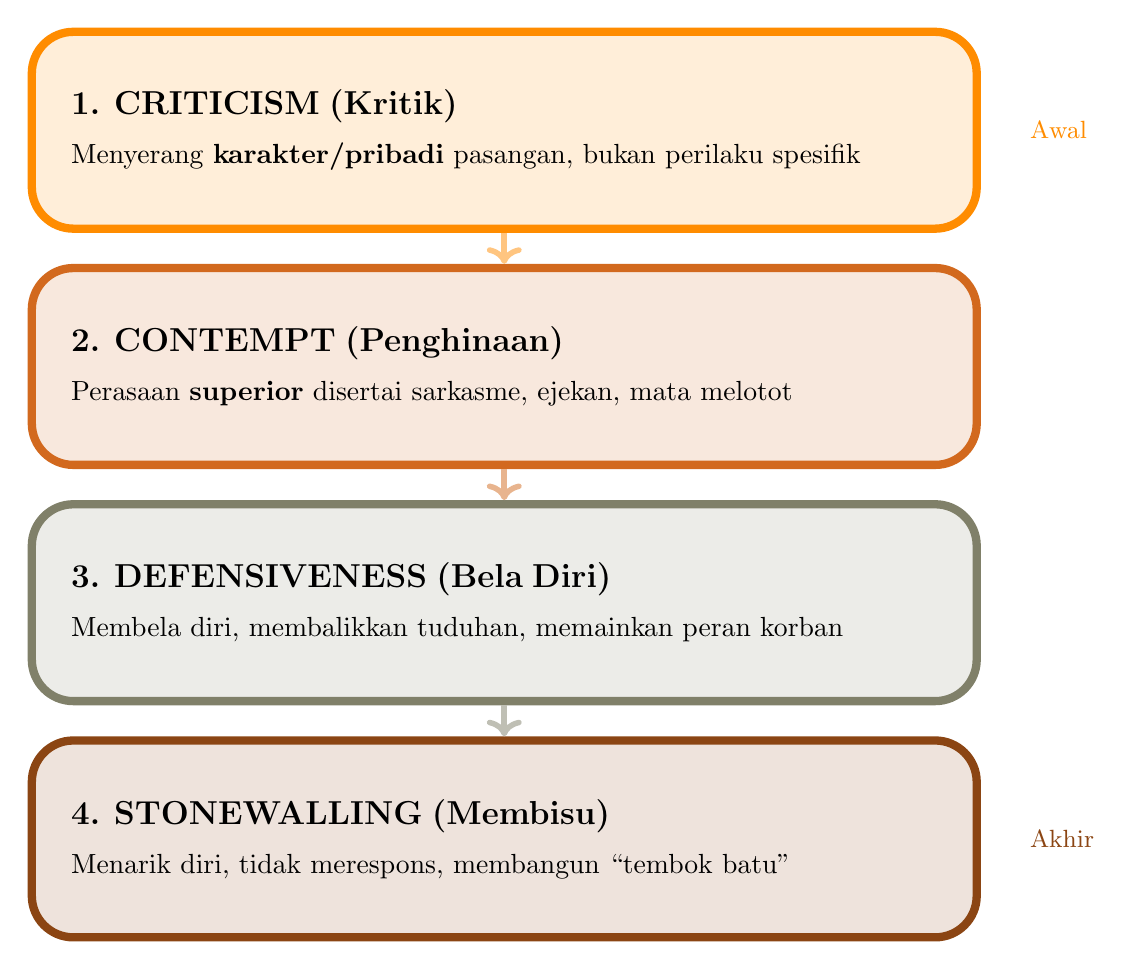
\begin{tikzpicture}[
    horse/.style={draw=#1, line width=3pt, rounded corners=15pt,
                  fill=#1!15, minimum width=12cm, minimum height=2.5cm,
                  align=left, text width=11cm}
]
    \node[horse=accent] (critic) at (0,6) {
        \textbf{\large 1. CRITICISM (Kritik)}\\[0.2cm]
        Menyerang \textbf{karakter/pribadi} pasangan, bukan perilaku spesifik
    };
    
    \node[horse=secondary] (contempt) at (0,3) {
        \textbf{\large 2. CONTEMPT (Penghinaan)}\\[0.2cm]
        Perasaan \textbf{superior} disertai sarkasme, ejekan, mata melotot
    };
    
    \node[horse=warmgray] (defens) at (0,0) {
        \textbf{\large 3. DEFENSIVENESS (Bela Diri)}\\[0.2cm]
        Membela diri, membalikkan tuduhan, memainkan peran korban
    };
    
    \node[horse=primary] (stone) at (0,-3) {
        \textbf{\large 4. STONEWALLING (Membisu)}\\[0.2cm]
        Menarik diri, tidak merespons, membangun ``tembok batu''
    };
    
    % Arrows showing progression
    \draw[->, line width=2pt, accent!50] (critic.south) -- (contempt.north);
    \draw[->, line width=2pt, secondary!50] (contempt.south) -- (defens.north);
    \draw[->, line width=2pt, warmgray!50] (defens.south) -- (stone.north);
    
    % Label
    \node[right=0.5cm of critic, font=\small, accent] {Awal};
    \node[right=0.5cm of stone, font=\small, primary] {Akhir};
\end{tikzpicture}
\end{center}

\section{Horseman 1: Criticism (Kritik)}

\subsection{Bedakan: Complaint vs Criticism}

\begin{center}
\renewcommand{\arraystretch}{1.5}
\begin{tabular}{|>{\raggedright}p{6cm}|>{\raggedright\arraybackslash}p{9cm}|}
\hline
\rowcolor{sagegreen!20}
\textbf{COMPLAINT (Benar)} & \textbf{CRITICISM (Salah)} \\
\hline
\textit{``Aku marah kamu nggak sapu dapur. Kita sepakat gantian. Bisa tolong sekarang?''} & \textit{``Kenapa kamu selalu lupa? Aku benci harus selalu sapu. Kamu nggak peduli.''} \\
\hline
Fokus pada \textbf{perilaku spesifik} & Menyerang \textbf{karakter} (``selalu'', ``kamu nggak peduli'') \\
\hline
Ada 3 komponen: Perasaan + Situasi + Request & Global, menyeluruh, menghakimi \\
\hline
\end{tabular}
\end{center}

\subsection{Formula Complaint yang Benar}

\begin{praktikbox}[Struktur Complaint Sehat]
\textbf{``Aku [perasaan] ketika [situasi spesifik]. Aku butuh [request].''}

\textbf{Contoh:}
\begin{itemize}
    \item ``Aku \textbf{marah} ketika \textbf{kamu nggak sapu dapur semalam}. Aku butuh \textbf{kamu sapu sekarang}.''
    \item ``Aku \textbf{kecewa} ketika \textbf{kamu nggabarin aku kalo telat}. Aku butuh \textbf{kabarin minimal 30 menit sebelumnya}.''
    \item ``Aku \textbf{merasa diabaikan} ketika \textbf{kamu main HP saat aku bicara}. Aku butuh \textbf{kamu taruh HP dan dengarkan dulu 10 menit}.''
\end{itemize}
\end{praktikbox}

\subsection{Kata-kata Pembunuh}

Hindari kata-kata ini dalam konflik:
\begin{itemize}
    \item ``Kamu \textbf{selalu}...''
    \item ``Kamu \textbf{tidak pernah}...''
    \item ``Kamu \textbf{terlalu}...''
    \item ``\textbf{Kenapa} kamu...'' (terdengar seperti kritik)
    \item ``Apa yang \textbf{salah} denganmu?''
\end{itemize}

\section{Horseman 2: Contempt (Penghinaan)}

\subsection{Ini adalah yang Paling Berbahaya}

\begin{warningbox}[Contempt = Poison]
Contempt adalah \textbf{prediktor tunggal terkuat} perceraian. Ketika ada contempt, hubungan dalam bahaya serius.

\textbf{Tanda-tanda Contempt:}
\begin{itemize}
    \item Sarkasme, ejekan, name-calling
    \item Mata melotot, sneering (menyeringai menghina)
    \item Body language meremehkan (menyilang tangan, mata ke langit)
    \item Menyindir cara pasangan bicara/berpakaian/berperilaku
    \item Merasa ``aku lebih baik darimu''
\end{itemize}
\end{warningbox}

\subsection{Contoh Perilaku Contempt}

\begin{center}
\renewcommand{\arraystretch}{1.4}
\begin{tabular}{|>{\raggedright}p{6cm}|>{\raggedright\arraybackslash}p{9cm}|}
\hline
\rowcolor{accent!20}
\textbf{Konteks} & \textbf{Contempt dalam Aksi} \\
\hline
Uang & ``Kamu itu \textbf{manja} dan \textbf{tidak tahu bersyukur}. Aku berasal dari keluarga yang \textbf{tahu nilai uang}, beda sama kamu.'' \\
\hline
Kerja rumah & ``Ah, \textbf{gitu aja nggak bisa}. Dasar \textbf{bodoh} kamu ini.'' \\
\hline
Pekerjaan & ``\textbf{Ngabisin waktu} aja kerjaanmu itu. \textbf{Siapa sih yang peduli}.'' \\
\hline
\end{tabular}
\end{center}

\subsection{Antidot: Fondness and Admiration}

Satu-satunya antidot untuk contempt adalah \keyterm{Fondness and Admiration System}:

\begin{tipbox}[Cara Membangun Fondness]
\begin{enumerate}
    \item \textbf{Scan for positives:} Sengaja cari hal positif tentang pasangan
    \item \textbf{Express gratitude:} Ucapkan terima kasih setiap hari
    \item \textbf{Reminisce:} Ingat kenangan indah masa lalu
    \item \textbf{Pride:} Ungkapkan kebanggaan pada pasangan
    \item \textbf{Affection:} Tunjukkan kasih sayang secara teratur
\end{enumerate}
\end{tipbox}

\section{Horseman 3: Defensiveness (Bela Diri)}

\subsection{Bentuk-bentuk Defensiveness}

\begin{enumerate}
    \item \textbf{Innocent Victim:} ``Kenapa kamu selalu nyalahin aku?''
    \item \textbf{Reverse Blame:} ``Iya, tapi kamu juga...''
    \item \textbf{Excuse:} ``Aku nggak bisa karena...''
    \item \textbf{Whining:} ``Apa pun yang kulakukan nggak pernah cukup!''
\end{enumerate}

\subsection{Contoh Defensiveness}

\begin{praktikbox}[Dialog Defensiveness]
\textbf{Pasangan:} ``Kamu telat lagi hari ini.''

\textbf{Defensiveness:}
\begin{itemize}
    \item ``Ya iyalah, macet! Bukan salahku!'' (excuse)
    \item ``Kamu aja kemarin telat, kok nggak bilang?'' (reverse blame)
    \item ``Kenapa sih kamu selalu komplain mulu?!'' (innocent victim)
\end{itemize}

\textbf{Non-Defensiveness (Benar):}
\begin{itemize}
    \item ``Iya, maaf. Ada kecelakaan di tol. Aku harusnya kabarin.''
    \item ``Kamu kecewa ya? Maaf bikin kamu khawatir.''
\end{itemize}
\end{praktikbox}

\section{Horseman 4: Stonewalling (Membisu)}

\subsection{Apa itu Stonewalling?}

\keyterm{Stonewalling} adalah ketika seseorang menarik diri dari interaksi, tidak merespons, dan membangun ``tembok batu''.

\begin{warningbox}[Tanda-tanda Stonewalling]
\begin{itemize}
    \item Tidak ada kontak mata
    \item Tidak ada respons verbal (``uh-huh'', ``hmm'')
    \item Body language tertutup (memalingkan tubuh)
    \item Ekspresi wajah datar (``poker face'')
    \item Fisik meninggalkan ruangan
\end{itemize}
\end{warningbox}

\subsection{Kenapa Orang Stonewall?}

\begin{praktikbox}[Penyebab Stonewalling]
\textbf{85\% stonewaller adalah pria} --- bukan karena pria ``jelek'', tapi karena:
\begin{enumerate}
    \item \textbf{Fisiologis:} Pria lebih mudah ``flooded'' (sistem kardiovaskular lebih reaktif)
    \item \textbf{Recovery:} Pria butuh waktu lebih lama untuk pulih dari konflik
    \item \textbf{Protection:} Stonewalling adalah self-protection dari flooding
    \item \textbf{Learned behavior:} Dipetik dari pola orang tua
\end{enumerate}
\end{praktikbox}

\section{Flooding: Akar dari Stonewalling}

\subsection{Apa itu Flooding?}

\keyterm{Flooding} adalah kondisi fisiologis di mana tubuh dalam mode ``fight or flight'':

\begin{center}
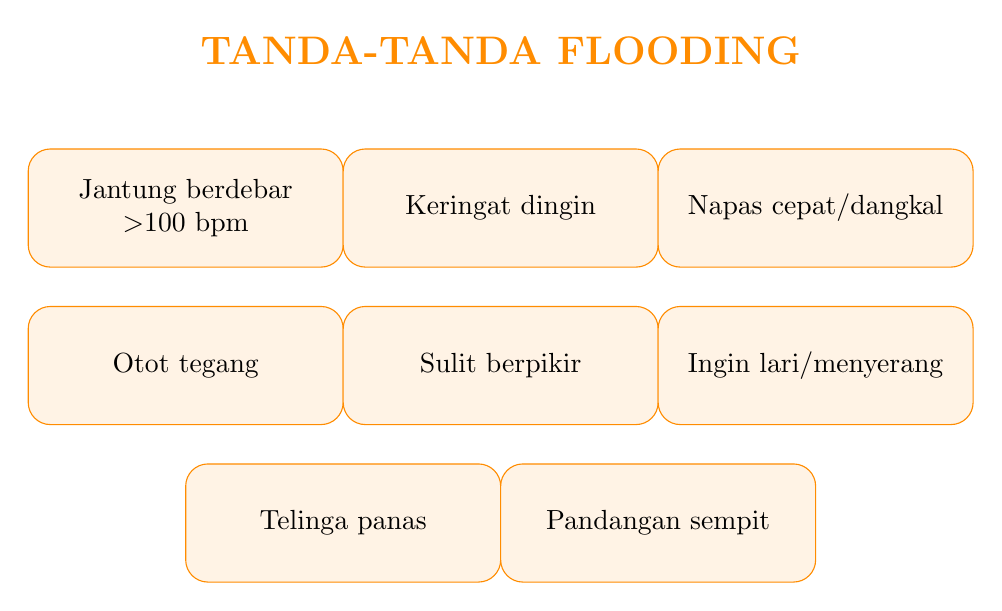
\begin{tikzpicture}[
    symptom/.style={draw=accent, rounded corners=8pt, fill=accent!10,
                    minimum width=4cm, minimum height=1.5cm, align=center}
]
    \node[font=\Large\bfseries, accent] at (0,4) {TANDA-TANDA FLOODING};
    
    \node[symptom] at (-4,2) {Jantung berdebar\\$>$100 bpm};
    \node[symptom] at (0,2) {Keringat dingin};
    \node[symptom] at (4,2) {Napas cepat/dangkal};
    \node[symptom] at (-4,0) {Otot tegang};
    \node[symptom] at (0,0) {Sulit berpikir};
    \node[symptom] at (4,0) {Ingin lari/menyerang};
    \node[symptom] at (-2,-2) {Telinga panas};
    \node[symptom] at (2,-2) {Pandangan sempit};
\end{tikzpicture}
\end{center}

\section{SAFE WORD/EMOJI SYSTEM (Prioritas Tinggi)}

\begin{insightbox}
\textbf{Ini adalah tools paling penting dalam bab ini.} Safe word/emoji memungkinkan kalian berkomunikasi saat kata-kata sudah tidak bisa digunakan.
\end{insightbox}

\subsection{Konsep Safe Word}

\begin{praktikbox}[Apa itu Safe Word?]
\textbf{Safe word} adalah kata atau sinyal yang disepakati untuk:
\begin{enumerate}
    \item Menyampaikan ``Aku flooded dan butuh break'' tanpa menjelaskan panjang lebar
    \item Menghentikan spiral negatif \textbf{sebelum} terlalu parah
    \item Memberi ruang untuk self-soothe
    \item Menjaga respect dan safety dalam konflik
\end{enumerate}
\end{praktikbox}

\subsection{Jenis-jenis Safe Signal}

\begin{center}
\renewcommand{\arraystretch}{1.5}
\begin{tabular}{|>{\raggedright}p{3cm}|>{\raggedright}p{5cm}|>{\raggedright\arraybackslash}p{7cm}|}
\hline
\rowcolor{primary!20}
\textbf{Tipe} & \textbf{Contoh} & \textbf{Kapan Digunakan} \\
\hline
\textbf{Safe Word} & ``Pineapple'', ``Kuning'', ``Time-out'' & Saat mulai merasa flooded \\
\hline
\textbf{Safe Emoji} & \emoji{\faPause}, \emoji{\faHandPaper}, \emoji{\faLifeRing} & Saat chatting/texting \\
\hline
\textbf{Safe Gesture} & Mengangkat tangan, membuat ``T'' & Saat sudah terlalu emosional untuk bicara \\
\hline
\textbf{Safe Object} & Benda kecil khusus yang diletakkan & Signal ``Aku butuh waktu'' \\
\hline
\end{tabular}
\end{center}

\subsection{Contoh Safe Word/Emoji System}

\begin{exercisebox}[Membuat Safe System Bersama]
\textbf{Langkah 1: Pilih Safe Word}
\begin{itemize}
    \item Pilih kata yang \textbf{tidak biasa} dalam percakapan kalian
    \item Hindari kata yang mungkin muncul di tengah konflik
    \item Contoh baik: ``Pineapple'', ``Blue moon'', ``Kode merah''
    \item Contoh buruk: ``Stop'', ``Cukup'', ``Sebentar''
\end{itemize}

\textbf{Langkah 2: Pilih Safe Emoji}
\begin{itemize}
    \item Saat chatting, gunakan emoji spesifik
    \item Contoh: \emoji{\faPause} = ``Aku overwhelmed, pause dulu''
    \item Contoh: \emoji{\faLifeRing} = ``Aku flooded butuh break''
    \item Contoh: \emoji{\faClock} = ``Aku butuh 20 menit, nanti balik''
\end{itemize}

\textbf{Langkah 3: Tetapkan Protokol}
\begin{itemize}
    \item Ketika safe word digunakan, \textbf{konflik langsung stop}
    \item Tidak ada ``tambahan kalimat terakhir''
    \item Kedua pihak pergi ke ruang terpisah
    \item Setelah 20-30 menit, kembali dan coba lagi
\end{itemize}
\end{exercisebox}

\subsection{Protokol Safe Word}

\begin{tipbox}[Cara Menggunakan Safe Word dengan Benar]
\textbf{Ketika kamu menggunakan safe word:}
\begin{enumerate}
    \item Katakan dengan jelas (``Aku pakai safe word: Pineapple'')
    \item Jelaskan secara singkat kenapa (opsional tapi bagus): ``Aku flooded, jantungku berdebar''
    \item Katakan kapan kamu akan kembali: ``Aku butuh 20 menit''
    \item Pergi ke ruang lain
    \item Lakukan self-soothing
    \item Kembali tepat waktu yang dijanjikan
\end{enumerate}

\textbf{Ketika pasangan menggunakan safe word:}
\begin{enumerate}
    \item \textbf{Respek segera} --- stop bicara meski kamu ``hampir selesai''
    \item Jangan kejar (don't pursue)
    \item Jangan anggap personal (``Dia nggak peduli pendapatku'')
    \item Manfaatkan waktu untuk self-soothe juga
    \item Siap mendengar saat dia kembali
\end{enumerate}
\end{tipbox}

\subsection{Self-Soothing saat Break}

\begin{praktikbox}[Aktivitas Self-Soothing yang Efektif]
\textbf{Fisiologis:}
\begin{itemize}
    \item Deep breathing (4-7-8)
    \item Progressive muscle relaxation
    \item Mandi air hangat
    \item Jalan-jalan ringan
    \item Minum air hangat
\end{itemize}

\textbf{Mental:}
\begin{itemize}
    \item Meditasi atau mindfulness
    \item Baca buku ringan
    \item Dengarkan musik menenangkan
    \item Tulis jurnal perasaan
\end{itemize}

\textbf{Yang TIDAK boleh dilakukan:}
\begin{itemize}
    \item Ruminate (muter-muter pikiran negatif)
    \item Stalking sosial media pasangan
    \item Hubungi teman untuk ``curhat'' (ini malah memperkuat negativity)
    \item Alkohol atau zat
\end{itemize}
\end{praktikbox}

\section{Antidot Lengkap untuk Four Horsemen}

\begin{center}
\renewcommand{\arraystretch}{1.5}
\begin{tabular}{|>{\raggedright}p{3cm}|>{\raggedright}p{4.5cm}|>{\raggedright\arraybackslash}p{7.5cm}|}
\hline
\rowcolor{primary!20}
\textbf{Horseman} & \textbf{Antidot} & \textbf{Contoh Praktis} \\
\hline
\textbf{Criticism} & \textbf{Gentle Start-up} & ``Aku marah karena...'' (bukan ``Kamu selalu...'') \\
\hline
\textbf{Contempt} & \textbf{Fondness \& Admiration} & Sebutkan 3 hal yang kamu hargai tentang pasangan setiap hari \\
\hline
\textbf{Defensiveness} & \textbf{Take Responsibility} & ``Sebagian ini salahku...'' \\
\hline
\textbf{Stonewalling} & \textbf{Safe Word + Self-Soothe} & ``Aku pakai safe word. Aku butuh 20 menit.'' \\
\hline
\end{tabular}
\end{center}

\section{Action Steps}

\begin{exercisebox}[To-Do: Setup Safe System]
\textbf{Hari ini:} Diskusikan dengan pasangan
\begin{enumerate}
    \item ``Apakah kita pernah mengalami flooding? Kapan?''
    \item ``Bagaimana biasanya kita bereaksi saat flooded?''
    \item ``Apakah ada Four Horsemen yang sering muncul dalam konflik kita?''
\end{enumerate}

\textbf{Buat kesepakatan:}
\begin{enumerate}
    \item Pilih safe word bersama
    \item Pilih safe emoji untuk chat
    \item Tulis protokol dan tempel di kulkas
    \item Latihan: Role-play menggunakan safe word
\end{enumerate}

\textbf{Protokol yang ditulis:}
\begin{itemize}
    \item Safe word kami: \rule{5cm}{0.4pt}
    \item Safe emoji: \rule{3cm}{0.4pt}
    \item Waktu break: \rule{3cm}{0.4pt} menit
    \item Aktivitas self-soothe: \rule{8cm}{0.4pt}
\end{itemize}
\end{exercisebox}

\chapter{Menerima Pengaruh: Power Sharing dalam Hubungan}

\begin{insightbox}
\textit{``Hubungan yang sehat bukanlah tentang siapa yang benar, tapi tentang bagaimana kita saling menghargai perspektif. Menerima pengaruh adalah fondasi dari kekuasaan bersama.''} — Dr. John Gottman
\end{insightbox}

\section{Apa itu Menerima Pengaruh?}

\keyterm{Menerima pengaruh} adalah kemampuan untuk membuka diri terhadap perspektif, perasaan, dan kebutuhan pasangan---terutama saat berkonflik. Ini bukan berarti selalu mengalah atau kehilangan diri sendiri, melainkan memiliki sikap keterbukaan: \textit{``Mungkin kamu punya poin yang valid. Mari kita diskusikan.''}

\subsection{Kenapa Ini Penting?}

Penelitian Gottman yang melibatkan 130 pasangan baru menikah menemukan:

\begin{praktikbox}[Fakta Ilmiah]
\begin{itemize}
    \item Pria yang \textbf{menerima pengaruh} dari istrinya memiliki perkawinan yang \textbf{signifikan lebih bahagia}
    \item Pria yang \textbf{menolak pengaruh} istri memiliki \textbf{81\% kemungkinan lebih tinggi} untuk bercerai
    \item Kesenjangan gender ini terkait dengan \textbf{socialisasi tradisional}, bukan biologi
\end{itemize}
\end{praktikbox}

Ini bukan berarti wanita selalu benar atau pria selalu salah. Ini tentang \textbf{power dynamics}---bagaimana tradisi patriarkal sering mengajarkan pria untuk ``memimpin'' tanpa mendengarkan, yang justru merusak hubungan.

\section{Karateristik Menerima vs Menolak Pengaruh}

\begin{center}
\renewcommand{\arraystretch}{1.6}
\begin{tabular}{|>{\raggedright}p{6cm}|>{\raggedright\arraybackslash}p{7cm}|}
\hline
\rowcolor{primary!20}
\textbf{MENOLAK PENGARUH (Toxic)} & \textbf{MENERIMA PENGARUH (Healthy)} \\
\hline
``Aku tahu apa yang terbaik'' & ``Ceritakan pemikiranmu'' \\
\hline
Memotong pembicaraan pasangan & Mendengarkan sampai selesai \\
\hline
Meyakinkan pasangan salah & Mencari validity dalam argumen pasangan \\
\hline
Body language defensive (mencibir, mata guling) & Body language terbuka (kontak mata, angguk) \\
\hline
Mengabaikan perasaan pasangan & Validasi: ``Aku mengerti kamu merasa...'' \\
\hline
Kompetisi: harus menang & Kolaborasi: mencari win-win \\
\hline
Menyalahkan pasangan & Mengambil tanggung jawab pribadi \\
\hline
Menggunakan kekerasan/emosi untuk kontrol & Menggunakan diskusi untuk solusi \\
\hline
\end{tabular}
\end{center}

\section{Self-Assessment: Seberapa Terbuka Kamu?}

\begin{exercisebox}[Test: Tingkat Keterbukaan Terhadap Pengaruh]
\textbf{Petunjuk:} Jawab setiap pertanyaan dengan skala 1-5 (1 = Tidak pernah, 5 = Selalu)

\begin{enumerate}[leftmargin=*]
    \item Saat pasangan mengajukan pendapat berbeda, aku benar-benar mendengarkan tanpa memotong.
    \item Aku bisa mengubah pendapatku jika pasangan memberikan argumen yang kuat.
    \item Saat konflik, aku bertanya ``Apa yang kamu butuhkan?'' sebelum memaksakan keinginanku.
    \item Aku mengakui kesalahanku dan meminta maaf dengan tulus.
    \item Aku menghormati perasaan pasangan meski logika mengatakan sebaliknya.
    \item Aku tidak merasa ``kalah'' saat mengikuti saran pasangan.
    \item Aku mencari middle ground daripada insist pada solusiku sendiri.
    \item Saat pasangan mengkritik, aku mencari kebenarannya bukannya defensive.
    \item Aku melibatkan pasangan dalam keputusan besar (finansial, karir, dll).
    \item Aku bisa bilang ``Kamu benar'' tanpa merasa terancam.
    \item Saat pasangan marah, aku tetap tenang dan mencari tahu akar masalahnya.
    \item Aku menghargai keahlian pasangan di bidang yang bukan kekuatanku.
\end{enumerate}

\textbf{Scoring:}
\begin{itemize}
    \item \textbf{48-60:} Excellent --- Kamu ahli dalam power sharing
    \item \textbf{36-47:} Good --- Ada ruang untuk improvement
    \item \textbf{24-35:} Fair --- Perlu kerja keras dalam area ini
    \item \textbf{12-23:} Needs Work --- Risiko hubungan tinggi tanpa perubahan
\end{itemize}
\end{exercisebox}

\section{Mengapa Pria Cenderung Menolak Pengaruh?}

\begin{warningbox}[Bukan Salah Pria Secara Individual]
Ini adalah \textbf{socialization issue}---bagaimana budaya membentuk ekspektasi gender, bukan kegagalan pribadi.
\end{warningbox}

\subsection{Faktor Budaya dan Sosial}

\begin{enumerate}[leftmargin=*]
    \item \textbf{Socialization Masculine:} Sejak kecil, laki-laki diajarkan untuk ``kuat'', ``tidak menyerah'', ``memimpin''---sering diartikan sebagai tidak boleh dipengaruhi.
    
    \item \textbf{Power = Identity:} Bagi banyak pria, kemampuan mengendalikan situasi terkait dengan self-worth. Menerima pengaruh terasa seperti kehilangan identitas.
    
    \item \textbf{Fear of Appeasing:} Takut dianggap `` whipped'' atau ``tidak berprinsip'' jika mengikuti pasangan.
    
    \item \textbf{Logical Processing:} Pria cenderung lebih fokus pada logika dan solusi, mengabaikan emotional content yang sering jadi inti argument wanita.
    
    \item \textbf{Conflict as Competition:} Olahraga/bidang kompetitif mengajarkan ``menang adalah segalanya'', sehingga konflik dianggap pertandingan.
\end{enumerate}

\subsection{Paradoksnya}

Paradoksnya: \textbf{Pria yang menerima pengaruh justru dihormati lebih} oleh pasangannya. Mereka dilihat sebagai:\
$\bullet$ Lebih dewasa emotionally\\
$\bullet$ Lebih confident (karena secure people don't need to control)\\
$\bullet$ Lebih menarik secara romantis\\
$\bullet$ Role model yang lebih baik untuk anak

\section{Cara Menerima Pengaruh: Step-by-Step}

\begin{praktikbox}[Framework: DEAR untuk Menerima Pengaruh]
\begin{enumerate}[leftmargin=*]
    \item \textbf{D}elay --- Tahan diri 6 detik sebelum merespons
    \item \textbf{E}xplore --- Tanyakan: ``Ceritakan lebih lanjut'' atau ``Apa yang kamu butuhkan?''
    \item \textbf{A}cknowledge --- Validasi: ``Aku mengerti kamu merasa...''
    \item \textbf{R}espond --- Berikan respon yang menunjukkan kamu mempertimbangkan
\end{enumerate}
\end{praktikbox}

\subsection{Frase-frase yang Menerima Pengaruh}

\begin{tipbox}[Kalimat Pembuka Keterbukaan]
\begin{itemize}
    \item ``Itu perspektif yang belum aku pikirkan.''
    \item ``Kamu punya poin yang valid.''
    \item ``Aku salah. Kamu benar.''
    \item ``Bagaimana kalau kita coba cara kamu?''
    \item ``Aku lihat kenapa kamu merasa begitu.''
    \item ``Mari cari solusi yang works untuk kita berdua.''
    \item ``Apa yang bisa aku lakukan untuk membantu?''
    \item ``Ceritakan lebih banyak tentang apa yang kamu rasakan.''
\end{itemize}
\end{tipbox}

\section{Attachment Styles dan Menerima Pengaruh}

\begin{center}
\renewcommand{\arraystretch}{1.5}
\begin{tabular}{|>{\raggedright}p{2.5cm}|>{\raggedright}p{5cm}|>{\raggedright\arraybackslash}p{5.5cm}|}
\hline
\rowcolor{primary!20}
\textbf{Attachment} & \textbf{Biasanya} & \textbf{Strategi Mengatasi} \\
\hline
\textbf{Anchor} & Naturally good at accepting influence; balance give-take & Lanjutkan, bantu pasangan yang struggle \\
\hline
\textbf{Island} & Resist influence (fear of losing autonomy); logical defense & Latihan: Acknowledge feelings first, then discuss logic \\
\hline
\textbf{Wave} & May accept too much influence (people-pleasing) then resent & Set boundaries; practice saying ``I need'' not just ``Okay'' \\
\hline
\end{tabular}
\end{center}

\section{Kapan Menolak Pengaruh adalah Wajar?}

\begin{warningbox}[Bukan Selalu Mengalah]
Menerima pengaruh \textbf{bukan} berarti:
\begin{itemize}
    \item Mengikuti segala permintaan pasangan tanpa batas
    \item Mengorbankan values atau principles fundamental
    \item Toleransi terhadap abuse atau manipulasi
    \item Kehilangan identitas diri
\end{itemize}
\end{warningbox}

\subsection{Menolak Pengaruh Secara Sehat}

Ada cara menolak yang tetap menghargai:
\begin{enumerate}[leftmargin=*]
    \item \textbf{Acknowledge dulu:} ``Aku mengerti kenapa kamu ingin ini.''
    \item \textbf{Jelaskan batasan:} ``Tapi ada sesuatu yang tidak bisa aku kompromikan.''
    \item \textbf{Tawarkan alternatif:} ``Bagaimana kalau...''
\end{enumerate}

\begin{exercisebox}[Latihan: Accepting Influence Practice]
\textbf{Skenario:} Pasanganmu ingin menghabiskan liburan dengan keluarganya, sedangkan kamu ingin liburan berdua.

\textbf{Respon yang Menolak Pengaruh:}
\begin{itemize}
    \item[$\square$] ``Keluargamu memang selalu lebih penting.''
    \item[$\square$] ``Aku sudah bilang berdua, jadi berdua.''
    \item[$\square$] ``Kamu tidak pernah menghargai keinginanku.''
\end{itemize}

\textbf{Respon yang Menerima Pengaruh:}
\begin{itemize}
    \item[$\square$] ``Aku mengerti kamu kangen keluarga.''
    \item[$\square$] ``Bagaimana kalau kita bagi: 3 hari keluarga, 4 hari berdua?''
    \item[$\square$] ``Apa yang membuat liburan keluarga penting bagimu tahun ini?''
\end{itemize}

\textbf{Latihan:} Diskusikan dengan pasangan: \textit{``Apa satu area di mana kamu merasa sulit menerima pengaruhku?''}
\end{exercisebox}

\section{Ringkasan Actionable}

\begin{tipbox}[Daily Practices]
\begin{enumerate}
    \item \textbf{Morning Check:} Sebelum memutuskan sesuatu, tanyakan pendapat pasangan.
    \item \textbf{Active Listening:} Saat pasangan bicara, tahan diri 6 detik sebelum merespons.
    \item \textbf{Acknowledgment Log:} Setiap hari, akui satu hal yang pasangan benar tentang.
    \item \textbf{Weekly Review:} Tanyakan ``Apa yang bisa aku lakukan lebih baik dalam mendengarkanmu?''
\end{enumerate}
\end{tipbox}

\chapter{Solvable vs Perpetual Problems: Masalah yang Bisa vs Tidak Bisa Diselesaikan}

\begin{insightbox}
\textit{``69\% konflik pernikahan adalah perpetual --- tidak akan pernah terselesaikan sepenuhnya. Pasangan bahagia bukan yang tanpa konflik, melainkan yang tahu cara \highlight{mengelola} konflik dengan bijaksana. Rahasianya bukan memenangkan pertarungan, tapi memahami perangnya.''}
\end{insightbox}

\section{Paradigma Baru: Dua Dunia Masalah yang Berbeda}

Dr. John Gottman, setelah meneliti ribuan pasangan selama lebih dari 40 tahun, menemukan fakta yang mengejutkan: \textbf{kebanyakan pasangan salah memahami konflik mereka}. Mereka memperlakukan setiap perbedaan sebagai masalah yang harus ``dipecahkan'' --- padahal ada dua kategori masalah yang sangat berbeda dalam hubungan.

\begin{praktikbox}[Revolusi Pemikiran Gottman]
Sebelum Gottman, terapi pernikahan berfokus pada ``problem-solving'' --- mencari solusi untuk setiap konflik. Gottman membuktikan bahwa pendekatan ini:\
\begin{itemize}
    \item \textbf{Gagal} pada 69\% kasus karena masalahnya memang \textbf{tidak ada solusinya}
    \item Membuat pasangan frustrasi dan merasa gagal
    \item Mengabaikan makna simbolik di balik perbedaan
\end{itemize}
\textit{Solusinya: Bedakan dulu masalahnya, baru tentukan strateginya.}
\end{praktikbox}

\subsection{Mengapa Pemahaman Ini Menyelamatkan Hubungan}

Tanpa pemahaman ini:
\begin{itemize}
    \item Kamu menghabiskan energi mencari ``solusi'' yang tidak ada
    \item Merasa frustrasi karena pasangan ``tidak mengerti''
    \item Menyimpulkan bahwa hubunganmu ``gagal'' karena konflik terus berulang
    \item Akhirnya menyerah: ``Kita tidak cocok''
\end{itemize}

Dengan pemahaman ini:
\begin{itemize}
    \item Kamu \textbf{menerima} bahwa beberapa perbedaan adalah bagian dari hubungan
    \item Fokus pada \textbf{mengelola} konflik, bukan menghilangkannya
    \item Melihat perbedaan sebagai sumber \textbf{pertumbuhan}, bukan ancaman
    \item Membangun kedekatan dari pemahaman, bukan kesamaan
\end{itemize}

\section{69\% Statistic: Kenapa Kebanyakan Konflik Abadi}

\subsection{Penelitian Gottman yang Mengubah Segalanya}

Dalam studi longitudinal yang melacak pasangan selama 14 tahun, Gottman menemukan:

\begin{center}
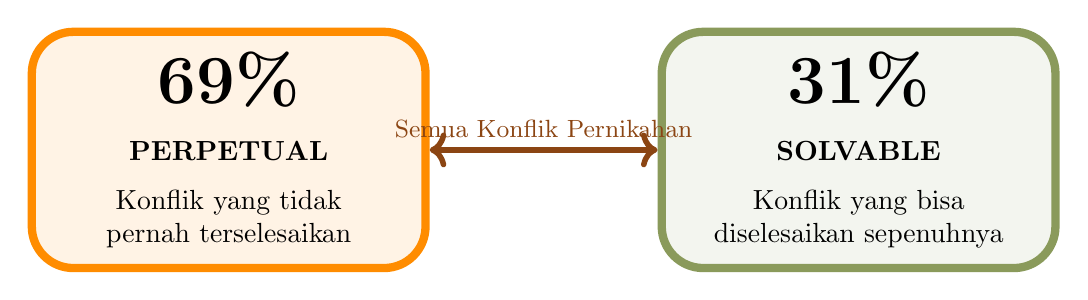
\begin{tikzpicture}[
    stat/.style={draw=#1, line width=3pt, rounded corners=15pt,
                 fill=#1!10, minimum width=5cm, minimum height=3cm, align=center}
]
    \node[stat=accent] (perpetual) at (-4,0) {
        \textbf{\Huge 69\%}\\[0.3cm]
        \textbf{PERPETUAL}\\[0.2cm]
        Konflik yang tidak\\pernah terselesaikan
    };
    
    \node[stat=sagegreen] (solvable) at (4,0) {
        \textbf{\Huge 31\%}\\[0.3cm]
        \textbf{SOLVABLE}\\[0.2cm]
        Konflik yang bisa\\diselesaikan sepenuhnya
    };
    
    \draw[<->, line width=2pt, primary] (perpetual) -- (solvable) node[midway, above, font=\small] {Semua Konflik Pernikahan};
\end{tikzpicture}
\end{center}

\subsection{Mengapa 69\%? Dasar Psikologisnya}

Angka ini bukan kebetulan. Ini mencerminkan \textbf{fakta fundamental} tentang manusia:

\begin{enumerate}
    \item \textbf{Kepribadian Stabil:} Trait dasar seperti ekstroversi, neuroticism, openness stabil sepanjang hidup
    \item \textbf{Nilai Terbentuk di Masa Kecil:} Konsep tentang uang, waktu, kebersihan, parenting tertanam dalam
    \item \textbf{Attachment Style:} Cara kita terhubung dengan orang lain sulit diubah total
    \item \textbf{Kebutuhan Dasar Berbeda:} Setiap orang punya level kebutuhan akan kedekatan, ruang, struktur yang berbeda
\end{enumerate}

\begin{tipbox}[Implikasi Praktis 69\%]
\begin{itemize}
    \item Jika kalian berkonflik tentang \textbf{topik yang sama} lebih dari 3 kali, kemungkinan besar itu \textbf{perpetual problem}
    \item Berhenti mencari ``solusi akhir'' --- itu seperti mencari kota fata morgana
    \item Alihkan fokus: dari ``bagaimana menyelesaikan'' ke ``bagaimana mengelola dengan baik''
\end{itemize}
\end{tipbox}

\subsection{Perbedaan Kunci dalam Perspektif}

\begin{insightbox}
\textbf{Paradoks Konflik:} Pasangan yang bahagia dan pasangan yang tidak bahagia memiliki \textbf{jumlah perpetual problem yang sama}. Perbedaannya bukan pada \textit{ada tidaknya} konflik, tapi pada \textit{cara menjalani} konflik tersebut.
\end{insightbox}

\section{Tabel Karakteristik Komprehensif: Solvable vs Perpetual}

Berikut adalah perbandingan detail lebih dari 10 dimensi kunci:

\begin{center}
\renewcommand{\arraystretch}{1.6}
\begin{tabular}{|>{\raggedright}p{3.2cm}|>{\raggedright}p{5.8cm}|>{\raggedright\arraybackslash}p{5.8cm}|}
\hline
\rowcolor{primary!20}
\textbf{Dimensi} & \textbf{SOLVABLE PROBLEMS} & \textbf{PERPETUAL PROBLEMS} \\
\hline
\textbf{1. Sifat Masalah} & Situasional dan konkret & Fundamental dan karakterologis \\
\hline
\textbf{2. Frekuensi} & Muncul sekali atau jarang & Berulang terus menerus \\
\hline
\textbf{3. Konteks} & Spesifik pada situasi tertentu & Muncul di berbagai konteks \\
\hline
\textbf{4. Makna Simbolik} & Minimal atau tidak ada & Sangat kaya dan dalam \\
\hline
\textbf{5. Solusi} & Ada solusi konkret dan clear & Tidak ada solusi ``benar'' \\
\hline
\textbf{6. Emosi Terlibat} & Emosi moderate dan terkontrol & Emosi intens dan personal \\
\hline
\textbf{7. Sejarah} & Terbatas pada hubungan ini & Sering terbawa dari masa lalu \\
\hline
\textbf{8. Area Terkait} & Satu area spesifik & Menyangkut banyak area hidup \\
\hline
\textbf{9. Respon Pasangan} & Kooperatif dalam problem-solving & Defensif dan protektif \\
\hline
\textbf{10. Potensi Resolusi} & 90-100\% bisa diselesaikan & 0\% diselesaikan, 100\% di-manage \\
\hline
\textbf{11. Efek Jangka Panjang} & Tidak mempengaruhi fondasi hubungan & Membentuk ``kebohongan jarak'' \\
\hline
\textbf{12. Kebutuhan Skill} & Problem-solving komunikasi & Dialogue dan empathy mendalam \\
\hline
\textbf{13. Tanda Sukses} & Masalah hilang/pergi & Masalah ada tapi tidak merusak \\
\hline
\textbf{14. Ancaman Hubungan} & Rendah jika diselesaikan & Tinggi jika menjadi gridlock \\
\hline
\end{tabular}
\end{center}

\subsection{Visual Perbandingan}

\begin{center}
\begin{tikzpicture}[
    solvable/.style={draw=sagegreen, line width=2pt, rounded corners=10pt, fill=sagegreen!10, minimum width=6cm, minimum height=5cm},
    perpetual/.style={draw=accent, line width=2pt, rounded corners=10pt, fill=accent!10, minimum width=6cm, minimum height=5cm}
]
    % Solvable Box
    \node[solvable] (sol) at (-4,0) {};
    \node[font=\Large\bfseries, sagegreen] at (-4,2) {SOLVABLE};
    \node[align=left, text width=5.5cm, font=\small] at (-4,0) {
        \faCheck\ Masalah spesifik\\[0.2cm]
        \faCheck\ Ada solusi konkret\\[0.2cm]
        \faCheck\ Emosi moderate\\[0.2cm]
        \faCheck\ Situasional\\[0.2cm]
        \faCheck\ Dapat diselesaikan
    };
    
    % Perpetual Box
    \node[perpetual] (per) at (4,0) {};
    \node[font=\Large\bfseries, accent] at (4,2) {PERPETUAL};
    \node[align=left, text width=5.5cm, font=\small] at (4,0) {
        \faExclamationTriangle\ Masalah berulang\\[0.2cm]
        \faExclamationTriangle\ Tidak ada solusi\\[0.2cm]
        \faExclamationTriangle\ Emosi intens\\[0.2cm]
        \faExclamationTriangle\ Fundamental\\[0.2cm]
        \faExclamationTriangle\ Hanya bisa di-manage
    };
\end{tikzpicture}
\end{center}

\section{Contoh Perbandingan dalam Kehidupan Nyata}

\begin{center}
\renewcommand{\arraystretch}{1.5}
\begin{tabular}{|>{\raggedright}p{2.5cm}|>{\raggedright}p{5cm}|>{\raggedright\arraybackslash}p{6.5cm}|}
\hline
\rowcolor{secondary!20}
\textbf{Topik} & \textbf{Solvable Problem} & \textbf{Perpetual Problem} \\
\hline
\textbf{Kecepatan Mengemudi} & Suami terburu-buru pagi karena istri lama siap-siap (situasi darurat) & Perbedaan gaya: safety vs efisiensi (terkait trust dan kontrol) \\
\hline
\textbf{Kebersihan} & Suami lupa buang sampah karena deadline kerja (situasional) & Perbedaan standar: chaos vs order (terkait nilai dan kenyamanan) \\
\hline
\textbf{Uang} & Mau beli equipment olahraga vs tabungan rumah (keputusan konkret) & Tabungan vs spending = security vs enjoyment (terkait childhood trauma) \\
\hline
\textbf{Waktu Bersama} & Suami lembur minggu ini untuk deadline (temporer) & Istri butuh quality time, suami butuh alone time (kebutuhan fundamental) \\
\hline
\textbf{Parenting} & Anak boleh main game berapa lama hari ini (keputusan spesifik) & Gaya parenting: disiplin ketat vs permisif (nilai dan keyakinan) \\
\hline
\textbf{Seks} & Belum mood malam ini karena capek (situasional) & Perbedaan libido dan definisi intimacy (kebutuhan dasar) \\
\hline
\textbf{Keluarga Besar} & Harus hadir acara keluarga minggu ini (spesifik) & Seberapa dekat dengan keluarga masing-masing (batasan dan identitas) \\
\hline
\textbf{Pekerjaan} & Butuh overtime minggu ini (temporer) & Ambisi karir vs work-life balance (prioritas hidup) \\
\hline
\end{tabular}
\end{center}

\section{Gridlock: Saat Perpetual Problem Macet dan Berbahaya}

\keyterm{Gridlock} adalah kondisi ketika perpetual problem tidak di-manage dengan baik, mengeras menjadi ``dinding'' yang memisahkan pasangan.

\subsection{Proses Terjadinya Gridlock}

\begin{center}
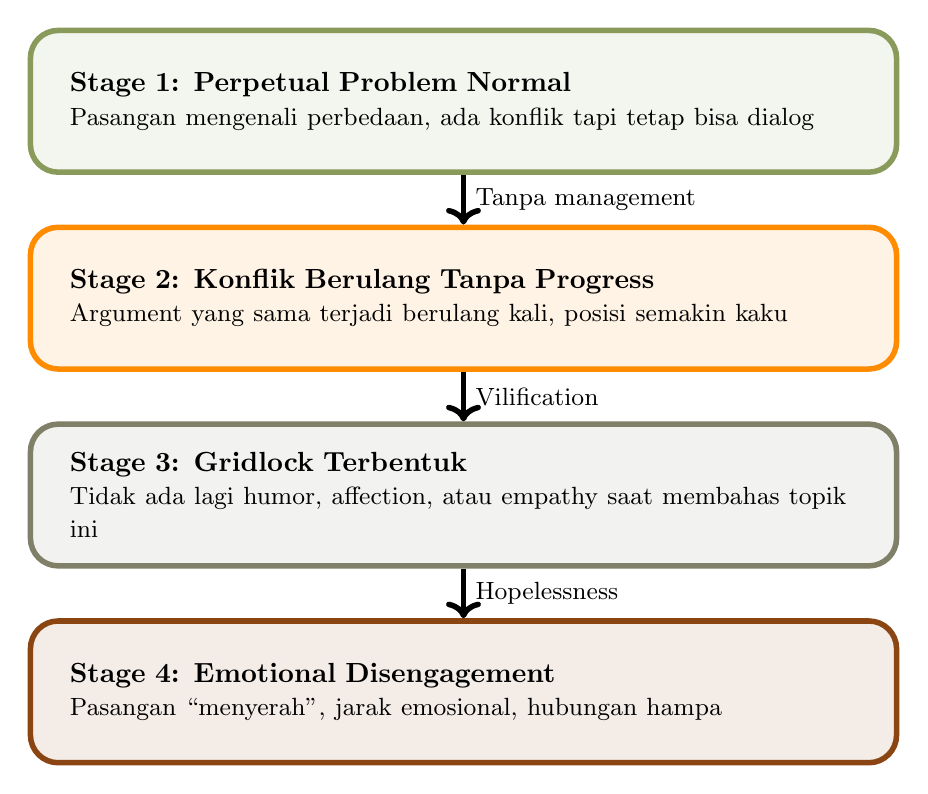
\begin{tikzpicture}[
    stage/.style={draw=#1, line width=2pt, rounded corners=10pt, fill=#1!10, 
                  minimum width=11cm, minimum height=1.8cm, align=left, text width=10cm}
]
    \node[stage=sagegreen] (s1) at (0,6) {
        \textbf{Stage 1: Perpetual Problem Normal}\\
        \small Pasangan mengenali perbedaan, ada konflik tapi tetap bisa dialog
    };
    
    \node[stage=accent] (s2) at (0,3.5) {
        \textbf{Stage 2: Konflik Berulang Tanpa Progress}\\
        \small Argument yang sama terjadi berulang kali, posisi semakin kaku
    };
    
    \node[stage=warmgray] (s3) at (0,1) {
        \textbf{Stage 3: Gridlock Terbentuk}\\
        \small Tidak ada lagi humor, affection, atau empathy saat membahas topik ini
    };
    
    \node[stage=primary] (s4) at (0,-1.5) {
        \textbf{Stage 4: Emotional Disengagement}\\
        \small Pasangan ``menyerah'', jarak emosional, hubungan hampa
    };
    
    \draw[->, line width=2pt] (s1) -- (s2) node[midway, right, font=\small] {Tanpa management};
    \draw[->, line width=2pt] (s2) -- (s3) node[midway, right, font=\small] {Vilification};
    \draw[->, line width=2pt] (s3) -- (s4) node[midway, right, font=\small] {Hopelessness};
\end{tikzpicture}
\end{center}

\subsection{Tanda-tanda Gridlock}

\begin{warningbox}[Tanda Gridlock yang Harus Diwaspadai]
\begin{itemize}
    \item \faExclamationTriangle\ \textbf{Konflik sama diulang berulang kali} tanpa kemajuan
    \item \faExclamationTriangle\ \textbf{Posisi semakin kaku} --- masing-masing tidak mau mengalah
    \item \faExclamationTriangle\ \textbf{Saling vilify} --- melihat pasangan sebagai ``jahat'' atau ``salah'
    \item \faExclamationTriangle\ \textbf{Tidak ada humor/affection} saat diskusi
    \item \faExclamationTriangle\ \textbf{Makin lama makin emosional} saat membahas topik
    \item \faExclamationTriangle\ \textbf{Akhirnya menghindari topik} sama sekali
    \item \faExclamationTriangle\ \textbf{Emotional disengagement} --- tidak peduli lagi
\end{itemize}

\textit{Gridlock adalah sinyal bahaya. Jika dibiarkan, hubungan akan menuju kehancuran.}
\end{warningbox}

\subsection{Dampak Gridlock pada Hubungan}

\begin{itemize}
    \item \textbf{Erosi Trust:} Kepercayaan hancur karena merasa tidak dipahami
    \item \textbf{Four Horsemen:} Criticism, Contempt, Defensiveness, Stonewalling muncul
    \item \textbf{Deadlock:} Tidak ada lagi room untuk negosiasi
    \item \textbf{Living as Roommates:} Hidup bersama tapi terpisah secara emosional
    \item \textbf{Risk of Infidelity:} Salah satu pihak mencari pemahaman di luar hubungan
\end{itemize}

\section{Dreams Within Conflict: Impian di Balik Perbedaan}

\subsection{Konsep Revolusioner Gottman}

Setiap perpetual problem menyembunyikan \keyterm{dreams} --- impian, nilai, kebutuhan, dan makna hidup yang fundamental bagi masing-masing pihak. Konflik yang tampaknya ``bodoh'' sebenarnya adalah \textbf{battle of dreams}.

\begin{insightbox}
\textit{``Di balik setiap perpetual problem, ada impian yang belum terwujud. Pasangan yang berhasil adalah yang mau mengeksplorasi dan menghormati impian pasangannya, meski impian itu bertentangan dengan impian mereka sendiri.''} --- John Gottman
\end{insightbox}

\subsection{Contoh Dreams dalam Konflik Umum}

\begin{center}
\renewcommand{\arraystretch}{1.5}
\begin{tabular}{|>{\raggedright}p{3cm}|>{\raggedright}p{4.5cm}|>{\raggedright}p{4.5cm}|>{\raggedright\arraybackslash}p{2.5cm}|}
\hline
\rowcolor{sagegreen!20}
\textbf{Topik Konflik} & \textbf{Dream Pasangan A} & \textbf{Dream Pasangan B} & \textbf{Nilai Dasar} \\
\hline
Anak & Merasa complete, legacy, kehangatan keluarga & Kebebasan, karir, spontanitas & Family vs Independence \\
\hline
Uang & Security, bebas dari anxiety masa kecil & Enjoyment, hidup sekarang & Safety vs Experience \\
\hline
Kebersihan & Order, kontrol, kenyamanan & Creativity, fleksibilitas & Structure vs Freedom \\
\hline
Waktu & Quality connection, intimacy & Personal space, recharge & Togetherness vs Alone \\
\hline
Pekerjaan & Achievement, recognition & Balance, kehadiran keluarga & Success vs Presence \\
\hline
Seks & Intimacy emosional, diterima & Physical release, stress relief & Connection vs Release \\
\hline
Rumah & Tempat istirahat yang sempurna & Tempat ekspresi kreatif & Perfection vs Expression \\
\hline
\end{tabular}
\end{center}

\subsection{Mengapa Dreams Penting}

\begin{praktikbox}[Mengapa Dreams Tidak Bisa Diabaikan]
\begin{enumerate}
    \item \textbf{Identitas:} Dreams adalah bagian dari siapa kita sebenarnya
    \item \textbf{Meaning-making:} Dreams memberi makna pada hidup
    \item \textbf{Resistence:} Mengorbankan dreams = mengorbankan diri sendiri
    \item \textbf{Conflict source:} Perbedaan dreams = sumber perpetual problem
\end{enumerate}

\textit{Solusi bukan meminta salah satu mengorbankan dreams-nya, tapi mencari \textbf{shared meaning} yang menghormati keduanya.}
\end{praktikbox}

\section{Self-Assessment: Identifikasi Jenis Masalahmu}

\begin{exercisebox}[Self-Assessment: Solvable atau Perpetual?]
\textbf{Petunjuk:} Pikirkan konflik utama yang sering terjadi dalam hubunganmu. Jawablah pertanyaan berikut dengan jujur.

\subsection*{BAGIAN A: Karakteristik Masalah}

\textbf{1. Seberapa sering konflik ini terjadi?}
\begin{itemize}
    \item[A] Jarang --- hanya dalam situasi spesifik
    \item[B] Sering --- pola yang berulang meski situasi berbeda
\end{itemize}

\textbf{2. Apakah ada solusi yang jelas?}
\begin{itemize}
    \item[A] Ya --- ada kompromi konkret yang bisa diterapkan
    \item[B] Tidak --- sepertinya tidak ada solusi yang memuaskan keduanya
\end{itemize}

\textbf{3. Seberapa intens emosi yang terlibat?}
\begin{itemize}
    \item[A] Moderate --- bisa didiskusikan tanpa terlalu emosional
    \item[B] Sangat intens --- menyentuh sesuatu yang sangat personal
\end{itemize}

\textbf{4. Apakah masalah ini terkait dengan nilai/masa kecil?}
\begin{itemize}
    \item[A] Tidak --- lebih tentang situasi sekarang
    \item[B] Ya --- berkaitan dengan pengalaman masa kecil atau nilai fundamental
\end{itemize}

\textbf{5. Bagaimana respon pasangan saat didiskusikan?}
\begin{itemize}
    \item[A] Kooperatif, mencari solusi bersama
    \item[B] Defensif, protektif, atau emosional
\end{itemize}

\subsection*{BAGIAN B: Deteksi Gridlock}

\textbf{6. Apakah kalian sering membahas topik yang sama tanpa kemajuan?}
\begin{itemize}
    \item[Ya] \textcolor{accent}{\textbf{[!]}} Tanda gridlock potensial
    \item[Tidak] Masih dalam tahap normal
\end{itemize}

\textbf{7. Apakah ada topik yang kalian hindari karena terlalu ``panas''?}
\begin{itemize}
    \item[Ya] \textcolor{accent}{\textbf{[!]}} Gridlock mungkin sudah terbentuk
    \item[Tidak] Masih bisa dialog
\end{itemize}

\textbf{8. Apakah kamu merasa pasangan ``tidak pernah mengerti''?}
\begin{itemize}
    \item[Ya] \textcolor{accent}{\textbf{[!]}} Emotional disengagement berkembang
    \item[Tidak] Masih ada harapan
\end{itemize}

\subsection*{SCORING}

\begin{center}
\renewcommand{\arraystretch}{1.4}
\begin{tabular}{|c|p{8cm}|}
\hline
\rowcolor{primary!20}
\textbf{Mayoritas Jawaban} & \textbf{Interpretasi} \\
\hline
A (BAGIAN A) & \textbf{SOLVABLE PROBLEM} --- Gunakan problem-solving skills standar \\
\hline
B (BAGIAN A) & \textbf{PERPETUAL PROBLEM} --- Fokus pada management dan dialogue \\
\hline
Ya (BAGIAN B) & \textbf{GRIDLOCK WARNING} --- Perlu intervensi segera \\
\hline
\end{tabular}
\end{center}
\end{exercisebox}

\section{Panduan Lengkap: Menyelesaikan Solvable Problems}

\subsection{5 Langkah Softened Startup}

\begin{tipbox}[Langkah 1: Softened Startup]
\begin{enumerate}
    \item \textbf{Start gentle:} ``Aku mau cerita tentang...'' bukan ``Kamu selalu...''
    \item \textbf{Complain, don't blame:} Fokus pada perilaku, bukan karakter
    \item \textbf{Describe, don't evaluate:} ``Sampah belum dibuang'' bukan ``Kamu malas''
    \item \textbf{Be polite:} Gunakan ``tolong'' dan ``terima kasih''
    \item \textbf{Give appreciations:} Mulai dengan yang positif
\end{enumerate}
\end{tipbox}

\subsection{Making and Receiving Repair Attempts}

\begin{center}
\renewcommand{\arraystretch}{1.4}
\begin{tabular}{|>{\raggedright}p{4cm}|>{\raggedright\arraybackslash}p{9cm}|}
\hline
\rowcolor{sagegreen!20}
\textbf{Tipe Repair} & \textbf{Contoh} \\
\hline
\textbf{I Feel Statement} & ``Aku merasa khawatir saat...'' \\
\hline
\textbf{Take Responsibility} & ``Aku salah, seharusnya aku...'' \\
\hline
\textbf{Apologize} & ``Maafkan aku sudah menyakitkanmu'' \\
\hline
\textbf{Agree} & ``Kamu benar tentang...'' \\
\hline
\textbf{Self-soothe} & ``Aku butuh menenangkan diri sebentar'' \\
\hline
\textbf{Affection} & Pelukan, sentuhan, humor lembut \\
\hline
\end{tabular}
\end{center}

\subsection{Step-by-Step Problem Solving}

\begin{praktikbox}[Proses 6 Langkah Problem Solving]
\textbf{Langkah 1: Define the Problem}
\begin{itemize}
    \item Masing-masing jelaskan perspektifnya (5 menit)
    \item Pasangan hanya mendengarkan, tidak interrupt
    \item Validasi: ``Jadi menurutmu...''
\end{itemize}

\textbf{Langkah 2: Brainstorm Solutions}
\begin{itemize}
    \item Buat daftar semua solusi yang mungkin
    \item Tidak ada kritik saat brainstorming
    \item Quantity over quality
\end{itemize}

\textbf{Langkah 3: Evaluate Options}
\begin{itemize}
    \item Bahas pro dan kontra masing-masing
    \item Cari solusi win-win atau kompromi
\end{itemize}

\textbf{Langkah 4: Choose a Solution}
\begin{itemize}
    \item Setujui satu solusi untuk dicoba
    \item Tentukan durasi trial period
\end{itemize}

\textbf{Langkah 5: Implement}
\begin{itemize}
    \item Jalankan solusi sesuai kesepakatan
    \item Dokumentasikan jika perlu
\end{itemize}

\textbf{Langkah 6: Follow-up}
\begin{itemize}
    \item Evaluasi setelah trial period
    \item Adjust jika perlu
\end{itemize}
\end{praktikbox}

\section{Panduan Lengkap: Mengelola Perpetual Problems}

\subsection{Paradigma Shift: From Solving to Managing}

\begin{insightbox}
\textbf{Paradoks Perpetual Problems:} Upaya untuk ``menyelesaikan'' perpetual problem justru akan memperburuknya. Strategi yang tepat adalah:
\begin{enumerate}
    \item \textbf{Accept:} Terima bahwa perbedaan ini akan selalu ada
    \item \textbf{Understand:} Pahami makna di balik posisi masing-masing
    \item \textbf{Dialogue:} Jalin dialog tentang dreams dan nilai
    \item \textbf{Compromise:} Temukan titik temu yang menghormati keduanya
    \item \textbf{Maintain:} Terus ``rawat'' dialog ini secara berkala
\end{enumerate}
\end{insightbox}

\subsection{Dreams Within Conflict Dialogue}

\begin{exercisebox}[Latihan Dreams Within Conflict]
\textbf{Tujuan:} Mengubah gridlock menjadi dialog tentang dreams

\textbf{Setup:}
\begin{itemize}
    \item Pilih perpetual problem yang belum menjadi gridlock total
    \item Pastikan kedua pihak dalam kondisi calm
    \item Siapkan 45-60 menit waktu tanpa gangguan
\end{itemize}

\textbf{Struktur Dialog:}

\textbf{Langkah 1: Speaker Shares Dreams (10 menit)}
\begin{itemize}
    \item Ceritakan tentang posisimu tanpa blame
    \item Jelaskan \textbf{mengapa} ini penting bagimu
    \item Hubungkan dengan pengalaman masa kecil/kebutuhan fundamental
    \item Contoh: ``Aku butuh banyak quality time karena di masa kecil...''
\end{itemize}

\textbf{Langkah 2: Listener Explores Dreams (10 menit)}
\begin{itemize}
    \item Tanyakan dengan rasa ingin tahu (curiosity)
    \item ``Ceritakan lebih tentang...''
    \item ``Kapan pertama kali kamu merasa ini penting?''
    \item ``Apa yang paling kamu takutkan jika kebutuhan ini tidak terpenuhi?''
\end{itemize}

\textbf{Langkah 3: Switch Roles (20 menit)}
\begin{itemize}
    \item Ulangi langkah 1-2 dengan posisi bertukar
\end{itemize}

\textbf{Langkah 4: Find Common Ground (10 menit)}
\begin{itemize}
    \item Identifikasi nilai/kebutuhan yang sama
    \item Brainstorm cara menghormati kedua dreams
    \item Buat agreement konkret
\end{itemize}
\end{exercisebox}

\subsection{Contoh Dialog Dreams Within Conflict}

\begin{center}
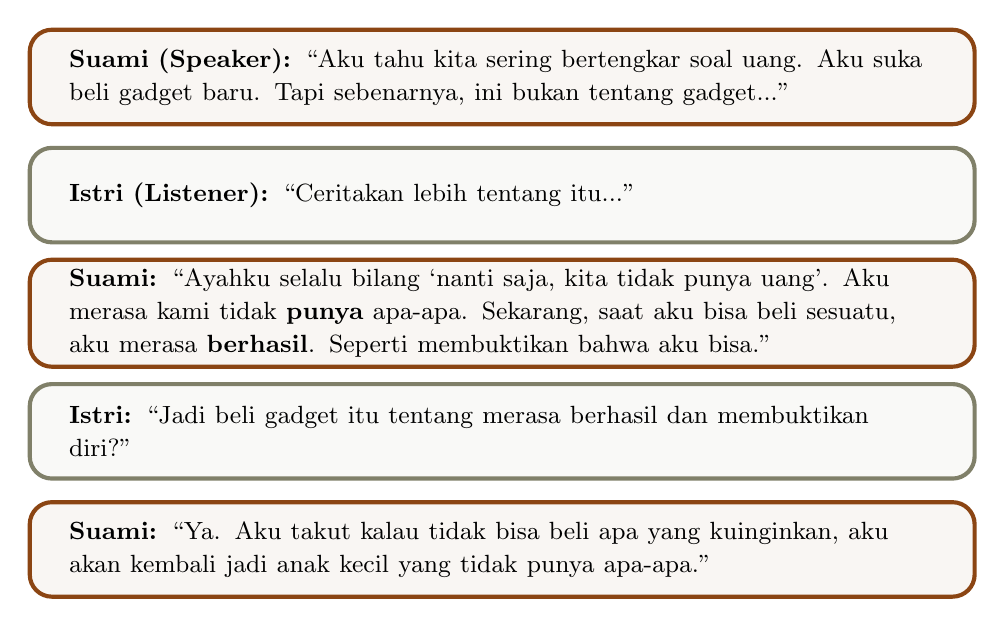
\begin{tikzpicture}[
    dialog/.style={draw=#1, line width=1.5pt, rounded corners=8pt, fill=#1!5,
                   minimum width=12cm, minimum height=1.2cm, align=left, text width=11cm}
]
    \node[dialog=primary] (d1) at (0,6) {
        \small\textbf{Suami (Speaker):} ``Aku tahu kita sering bertengkar soal uang. Aku suka beli gadget baru. Tapi sebenarnya, ini bukan tentang gadget...''
    };
    
    \node[dialog=warmgray] (d2) at (0,4.5) {
        \small\textbf{Istri (Listener):} ``Ceritakan lebih tentang itu...''
    };
    
    \node[dialog=primary] (d3) at (0,3) {
        \small\textbf{Suami:} ``Ayahku selalu bilang `nanti saja, kita tidak punya uang'. Aku merasa kami tidak \textbf{punya} apa-apa. Sekarang, saat aku bisa beli sesuatu, aku merasa \textbf{berhasil}. Seperti membuktikan bahwa aku bisa.''
    };
    
    \node[dialog=warmgray] (d4) at (0,1.5) {
        \small\textbf{Istri:} ``Jadi beli gadget itu tentang merasa berhasil dan membuktikan diri?''
    };
    
    \node[dialog=primary] (d5) at (0,0) {
        \small\textbf{Suami:} ``Ya. Aku takut kalau tidak bisa beli apa yang kuinginkan, aku akan kembali jadi anak kecil yang tidak punya apa-apa.''
    };
\end{tikzpicture}
\end{center}

\section{Topik Perpetual Problems Umum dan Strateginya}

\subsection{Uang: Security vs Enjoyment}

\begin{warningbox}[Konflik Uang]
\textbf{Saver (Hemat)}\ dreams: Keamanan, bebas anxiety, kontrol masa depan\\
\textbf{Spender (Habiskan)}\ dreams: Enjoyment, reward diri, hidup sekarang

\textbf{Strategi:}
\begin{itemize}
    \item Buat tiga bucket: Needs, Wants, Dreams
    \item Tetapkan persentase yang jelas untuk masing-masing
    \item ``Fun money'' --- masing-masing punya budget bebas tanpa pertanggungjawaban
    \item Review bersama setiap bulan
\end{itemize}
\end{warningbox}

\subsection{Seks: Intimacy vs Physical Release}

\begin{praktikbox}[Konflik Intimasi]
\textbf{High-desire partner}\ dreams: Connection, diterima, self-worth\\
\textbf{Low-desire partner}\ dreams: Kedekatan non-seksual, tidak merasa pressure

\textbf{Strategi:}
\begin{itemize}
    \item Scheduled intimacy --- jadwalkan tanpa terdengar ``tidak romantic''
    \item Non-sexual touch hari-hari non-intimacy
    \item Communicate needs tanpa pressure
    \item Eksplorasi apa yang membuat low-desire partner merasa dekat
\end{itemize}
\end{praktikbox}

\subsection{Parenting: Discipline vs Nurturing}

\begin{tipbox}[Konflik Parenting]
\textbf{Strict parent}\ dreams: Anak sukses, disiplin, siap dunia\\
\textbf{Lenient parent}\ dreams: Anak bahagia, kreatif, bebas

\textbf{Strategi:}
\begin{itemize}
    \item Private discussion --- jangan pernah bertengkar di depan anak
    \item United front --- kompromi dulu, baru implementasi
    \item Division of domain --- masing-masing lead di area tertentu
    \item Regular parenting meetings
\end{itemize}
\end{tipbox}

\subsection{Kebersihan: Order vs Chaos}

\begin{insightbox}[Konflik Kebersihan]
\textbf{Neat partner}\ dreams: Kontrol, kenyamanan, estetika\\
\textbf{Messy partner}\ dreams: Kreativitas, fleksibilitas, tidak obsesif

\textbf{Strategi:}
\begin{itemize}
    \item Zoning: Area bersama harus rapi, area pribadi bebas
    \item Systems, bukan blame: Buat sistem yang memudahkan
    \item Weekly reset: Waktu bersama merapikan
    \item Acceptance: Beberapa ketidaksempurnaan harus diterima
\end{itemize}
\end{insightbox}

\section{Integrasi dengan Attachment Styles}

\subsection{Bagaimana Masing-Masing Tipe Menangani Perpetual Problems}

\begin{center}
\renewcommand{\arraystretch}{1.6}
\begin{tabular}{|>{\raggedright}p{2.5cm}|>{\raggedright}p{5.5cm}|>{\raggedright\arraybackslash}p{5.5cm}|}
\hline
\rowcolor{primary!20}
\textbf{Tipe} & \textbf{Respon terhadap Perpetual Problem} & \textbf{Strategi Optimal} \\
\hline
\textbf{Anchor} & Tetap terbuka untuk dialog, tidak terlalu defensive, bisa melihat perspektif pasangan & Gunakan secure base untuk membantu pasangan merasa aman saat explore dreams \\
\hline
\textbf{Island} & Menjauh saat perpetual problem diangkat, merasa terjebak, avoid dialogue & Beri reassurance tidak akan dipaksa mengubah nilai, beri waktu proses \\
\hline
\textbf{Wave} & Emosional dan clingy saat perpetual problem muncul, fear abandonment & Validasi perasaan dulu, jangan biarkan merasa ditinggal saat dialog \\
\hline
\end{tabular}
\end{center}

\subsection{Kombinasi Tipe dan Perpetual Problems}

\begin{warningbox}[Kombinasi yang Paling Menantang]
\textbf{Island + Wave dalam Perpetual Problem:}
\begin{itemize}
    \item Saat perpetual problem muncul, Wave cling dan Island withdraw
    \item Ini memperkuat pola pursuer-distancer
    \item \textbf{Solusi:} Island harus belajar stay present, Wave harus belajar self-soothe
\end{itemize}

\textbf{Dua Island dalam Perpetual Problem:}
\begin{itemize}
    \item Keduanya withdraw, masalah tidak pernah dibahas
    \item Hubungan menjadi ``roommate'' arrangement
    \item \textbf{Solusi:} Scheduled dialogue wajib, jangan biarkan avoidance
\end{itemize}

\textbf{Dua Wave dalam Perpetual Problem:}
\begin{itemize}
    \item Konflik menjadi sangat emosional dan dramatis
    \item Testing behavior muncul
    \item \textbf{Solusi:} Grounding techniques, take turns speaking
\end{itemize}
\end{warningbox}

\section{Case Studies: Before and After}

\subsection{Case Study 1: Uang dan Gridlock}

\begin{praktikbox}[Case: David \& Sarah --- Gridlock Keuangan]
\textbf{BEFORE (Gridlock):}
\begin{itemize}
    \item David: Spender, suka beli gadget dan makan di restoran mahal
    \item Sarah: Saver, ingin tabungan rumah dan dana darurat besar
    \item Pola: Setiap kali David beli sesuatu, Sarah marah besar
    \item David mulai sembunyi-sembunyi belanja (financial infidelity)
    \item Sarah merasa tidak bisa percaya, mengontrol semua rekening
    \item Gridlock total --- tidak ada lagi dialogue
\end{itemize}

\textbf{INTERVENTI Dreams Within Conflict:}
\begin{itemize}
    \item David: ``Ayahku miskin, aku merasa tidak punya apa-apa. Beli gadget = merasa berhasil''
    \item Sarah: ``Orangtuaku bercerai karena utang. Tabungan = security aku tidak ditinggal''
\end{itemize}

\textbf{AFTER (Managed):}
\begin{itemize}
    \item Agreement: 60\% needs/tabungan, 20\% fun money masing-masing (tanpa pertanyaan), 20\% dreams
    \item David punya ``freedom account'' untuk gadget --- tidak perlu sembunyi
    \item Sarah puas dengan sistem otomatis tabungan
    \item Monthly money date untuk review dan connection
\end{itemize}
\end{praktikbox}

\subsection{Case Study 2: Waktu Bersama}

\begin{praktikbox}[Case: Mike \& Lisa --- Perpetual Time Problem]
\textbf{BEFORE:}
\begin{itemize}
    \item Lisa (Wave): Butuh quality time setiap hari, merasa diabaikan jika tidak
    \item Mike (Island): Butuh alone time setiap hari, merasa tercekik jika tidak
    \item Pola: Lisa nag $
ightarrow$ Mike withdraw $
ightarrow$ Lisa nag lebih keras $
ightarrow$ Mike menghilang
\end{itemize}

\textbf{DREAMS EXPLORED:}
\begin{itemize}
    \item Lisa: ``Di keluargaku, tidak ada yang benar-benar `melihat' aku. Quality time = aku ada dan dihargai''
    \item Mike: ``Orangtuaku selalu membutuhkan perhatianku. Alone time = aku bisa bernapas''
\end{itemize}

\textbf{AFTER:}
\begin{itemize}
    \item Structure: Mike pulang kerja $
ightarrow$ 1 jam alone time $
ightarrow$ quality time bersama
    \item Lisa belajar self-soothing saat Mike recharge
    \item Mike inisiatif quality time (bekerja sama kebutuhan Lisa)
    \item Weekend: 1 hari ``we time'', 1 hari ada alone time masing-masing
\end{itemize}
\end{praktikbox}

\section{Action Steps: Program 30 Hari}

\begin{exercisebox}[Program 30 Hari: Mastering Your Problems]

\textbf{MINGGU 1: Identification}
\begin{itemize}
    \item \textbf{Hari 1-2:} List semua konflik dalam 6 bulan terakhir
    \item \textbf{Hari 3-4:} Kategorikan: Solvable atau Perpetual? (gunakan assessment)
    \item \textbf{Hari 5-7:} Identifikasi tanda gridlock pada perpetual problems
\end{itemize}

\textbf{MINGGU 2: Solvable Problems}
\begin{itemize}
    \item \textbf{Hari 8-10:} Pilih satu solvable problem, lakukan 6-step problem solving
    \item \textbf{Hari 11-12:} Praktek softened startup dan repair attempts
    \item \textbf{Hari 13-14:} Review dan celebrate success
\end{itemize}

\textbf{MINGGU 3: Perpetual Problems --- Dreams Exploration}
\begin{itemize}
    \item \textbf{Hari 15-17:} Pilih satu perpetual problem yang belum gridlock
    \item \textbf{Hari 18-19:} Lakukan Dreams Within Conflict dialogue
    \item \textbf{Hari 20-21:} Dokumentasikan dreams masing-masing
\end{itemize}

\textbf{MINGGU 4: Integration dan Agreement}
\begin{itemize}
    \item \textbf{Hari 22-24:} Brainstorm agreement yang menghormati kedua dreams
    \item \textbf{Hari 25-26:} Implementasi trial agreement
    \item \textbf{Hari 27-28:} Check-in dan adjust
    \item \textbf{Hari 29-30:} Reflection dan planning forward
\end{itemize}
\end{exercisebox}

\section{Kesimpulan: Menerima dan Mengelola}

\begin{insightbox}
\textbf{Key Takeaway Chapter 7:}
\begin{enumerate}
    \item \textbf{69\% konflik adalah perpetual} --- ini normal, bukan tanda hubungan gagal
    \item \textbf{Solvable vs Perpetual memerlukan strategi berbeda}
    \item \textbf{Gridlock} adalah musuh sejati, bukan perpetual problem itu sendiri
    \item \textbf{Dreams within conflict} adalah kunci untuk mengelola perpetual problems
    \item \textbf{Pasangan bahagia} bukan yang tanpa konflik, tapi yang jago mengelola konflik
\end{enumerate}

\textit{``Tujuan bukan menghilangkan perbedaan, tapi belajar menari bersama perbedaan itu.''}
\end{insightbox}

\begin{tipbox}[Checklist Cepat: Apa yang Harus Diingat]
\begin{itemize}
    \item[$\square$] Cek: Apakah ini solvable atau perpetual?
    \item[$\square$] Kalau solvable: Gunakan 6-step problem solving
    \item[$\square$] Kalau perpetual: Explore dreams, jangan coba ``menyelesaikan''
    \item[$\square$] Hindari gridlock: Jaga dialogue tetap terbuka
    \item[$\square$] Integrasi dengan attachment style: Sesuaikan approach
    \item[$\square$] Review secara berkala: Perpetual problems perlu ``perawatan'' rutin
\end{itemize}
\end{tipbox}

\chapter{Upaya Perbaikan (Repair Attempts): Menghentikan Spiral Negatif}

\begin{insightbox}
\textit{``Pasangan bahagia juga bertengkar. Bedanya, mereka mahir dalam \textbf{repair attempts} --- sinyal-sinyal halus (maupun jelas) yang menghentikan konflik sebelum melukai. Tanpa kemampuan ini, pernikahan bagaikan mobil tanpa rem: cepat atau lambat akan celaka.''}
\end{insightbox}

\section{Apa itu Repair Attempt?}

\keyterm{Repair attempt} adalah \textbf{segala pernyataan atau tindakan} yang bertujuan menghentikan eskalasi negativitas selama konflik. Ini adalah ``rem darurat'' dalam hubungan --- cara untuk mengatakan \textit{``Stop, kita perlu mengurangi kecepatan sebelum terlambat.''}

\begin{praktikbox}[Definisi Repair Attempt]
Menurut penelitian Dr. John Gottman:
\begin{itemize}
    \item \textbf{Fungsi utama:} Mencegah negativitas meluap dari kontrol
    \item \textbf{Waktu:} Bisa dilakukan kapan saja selama konflik
    \item \textbf{Bentuk:} Bisa verbal, non-verbal, humor, atau fisik
    \item \textbf{Kunci:} Suksesnya bergantung pada \textbf{kekuatan persahabatan} di baliknya
\end{itemize}
\end{praktikbox}

\subsection{Analogi: Repair Attempt sebagai Rem Mobil}

Bayangkan mengemudi di jalan berliku:
\begin{itemize}
    \item \textbf{Tanpa rem:} Mobil akan terus melaju meski ada tikungan tajam --- celaka hanya masalah waktu
    \item \textbf{Rem tidak berfungsi:} Kamu tekan rem, tapi tidak terjadi apa-apa
    \item \textbf{Rem berfungsi baik:} Sekali tekan, mobil melambat dengan aman
\end{itemize}

Dalam hubungan:
\begin{itemize}
    \item \textbf{Tidak ada repair habit:} Konflik kecil jadi besar, besar jadi monster
    \item \textbf{Repair gagal:} Kamu mencoba memperbaiki, tapi pasangan tidak ``mendengar''
    \item \textbf{Repair sukses:} Konflik dihentikan, koneksi dipulihkan, solusi ditemukan
\end{itemize}

\section{Ilmu di Balik Repair Attempts}

\subsection{Prediktor Kekuatan Pernikahan}

Penelitian Gottman menemukan fakta mengejutkan:

\begin{warningbox}[Data Penelitian]
\begin{itemize}
    \item Keberhasilan \textbf{repair attempts} adalah salah satu \textbf{faktor utama} yang membedakan pernikahan yang berkembang vs yang gagal
    \item Kehadiran Empat Kuda Jelajah (Four Horsemen) memprediksi perceraian dengan akurasi 82\%
    \item \textbf{Tetapi} ketika ditambahkan \textbf{kegagalan repair attempts}, akurasi prediksi naik ke 90\%+
    \item Artinya: Pasangan bisa punya konflik intens, tapi jika repair attempts mereka berhasil, pernikahan tetap stabil
\end{itemize}
\end{warningbox}

\subsection{Feedback Loop: Konflik dan Repair}

\begin{center}
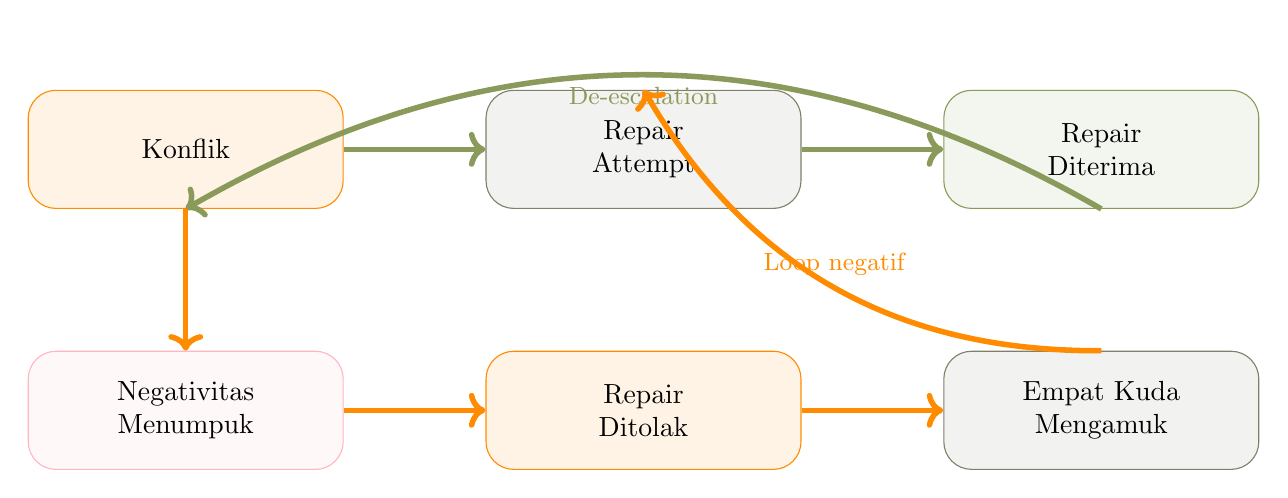
\begin{tikzpicture}[
    node distance=1.8cm,
    box/.style={draw=#1, rounded corners=10pt, fill=#1!10, 
                minimum width=4cm, minimum height=1.5cm, align=center},
    arrow/.style={->, line width=2pt}
]
    % Nodes
    \node[box=accent] (konflik) {Konflik};
    \node[box=warmgray, right=of konflik] (repair) {Repair\\Attempt};
    \node[box=sagegreen, right=of repair] (sukses) {Repair\\Diterima};
    \node[box=softpink, below=of konflik] (negatif) {Negativitas\\Menumpuk};
    \node[box=accent, right=of negatif] (gagal) {Repair\\Ditolak};
    \node[box=warmgray, right=of gagal] (4h) {Empat Kuda\\Mengamuk};
    
    % Arrows - Success path
    \draw[arrow, sagegreen] (konflik) -- (repair);
    \draw[arrow, sagegreen] (repair) -- (sukses);
    \draw[arrow, sagegreen, bend right=30] (sukses.south) to node[below, font=\small] {De-escalation} (konflik.south);
    
    % Arrows - Failure path
    \draw[arrow, accent] (konflik) -- (negatif);
    \draw[arrow, accent] (negatif) -- (gagal);
    \draw[arrow, accent] (gagal) -- (4h);
    \draw[arrow, accent, bend left=30] (4h.north) to node[above, font=\small] {Loop negatif} (repair.north);
\end{tikzpicture}
\end{center}

\begin{insightbox}
\textbf{Paradoks Repair Attempts:}

Pasangan dalam pernikahan bermasalah \textbf{justru lebih sering} mencoba repair attempts daripada pasangan bahagia. Tapi karena setiap repair gagal, mereka harus mencoba lagi dan lagi --- penuh kepanikan dan keputusasaan.

Bedanya: Dalam pernikahan bahagia, \textbf{satu} repair attempt sederhana cukup. Dalam pernikahan bermasalah, bahkan repair yang paling elegan pun ditolak.
\end{insightbox}

\section{Tipe-tipe Repair Attempts}

\subsection{1. Repair Verbal: Kata-kata yang Menyembuhkan}

\begin{center}
\renewcommand{\arraystretch}{1.6}
\begin{tabular}{|>{\raggedright}p{3.5cm}|>{\raggedright}p{5cm}|>{\raggedright\arraybackslash}p{6cm}|}
\hline
\rowcolor{primary!20}
\textbf{Kategori} & \textbf{Contoh Kalimat} & \textbf{Kapan Digunakan} \\
\hline
\textbf{Minta Maaf} & ``Maaf aku defensive tadi'' & Saat sadar reaksi berlebihan \\
\hline
\textbf{Minta Waktu} & ``Bisa kita pause 10 menit? Aku butuh menenangkan diri'' & Saat merasa flooding \\
\hline
\textbf{Validasi} & ``Aku mengerti kenapa kamu marah'' & Saat pasangan merasa tidak didengar \\
\hline
\textbf{Ambil Tanggung Jawab} & ``Ini salahku juga, aku ikut andil'' & Saat diskusi terasa menyalahkan \\
\hline
\textbf{Minta Ulang} & ``Bisa kita mulai ulang? Aku tidak mau bertengkar'' & Saat start-up terlalu keras \\
\hline
\textbf{Ingatkan Ikatan} & ``Kita tim, ingat? Aku cinta kamu'' & Saat konflik terasa personal \\
\hline
\textbf{Konteks Eksternal} & ``Ini bukan tentangmu, aku stres kerja'' & Saat emosi berasal dari faktor luar \\
\hline
\textbf{Tanya Perasaan} & ``Kamu merasa gimana sekarang?'' & Saat butuh mengalihkan ke empati \\
\hline
\textbf{Akui Usaha} & ``Aku tahu kamu cuma mau yang terbaik'' & Saat pasangan defensive \\
\hline
\textbf{Humor Ringan} & ``Kita kayak tetangga yang berantem lagi'' & Saat tensi masih bisa dijokeskan \\
\hline
\end{tabular}
\end{center}

\begin{tipbox}[20+ Frasa Repair Verbal]
\textbf{I FEEL (Mengekspresikan Emosi):}
\begin{enumerate}[itemsep=0.1cm]
    \item ``Aku merasa sedih...''
    \item ``Aku merasa tersakiti...''
    \item ``Aku merasa marah...''
    \item ``Aku merasa takut...''
    \item ``Aku merasa malu...''
    \item ``Aku merasa tidak dihargai...''
\end{enumerate}

\textbf{SORRY (Meminta Maaf):}
\begin{enumerate}[itemsep=0.1cm]
    \item ``Maaf, aku defensive tadi...''
    \item ``Maaf, aku tidak dengar dengan baik...''
    \item ``Maaf, aku melebih-lebihkan...''
    \item ``Maaf, aku membuat ini jadi personal...''
    \item ``Maaf, aku lebay tadi...''
\end{enumerate}

\textbf{NEED (Mengungkapkan Kebutuhan):}
\begin{enumerate}[itemsep=0.1cm]
    \item ``Aku butuh kamu mendengar dulu...''
    \item ``Aku butuh istirahat sebentar...''
    \item ``Aku butuh kamu percaya padaku...''
    \item ``Aku butuh pelukan...''
    \item ``Aku butuh waktu untuk berpikir...''
\end{enumerate}
\end{tipbox}

\subsection{2. Repair Non-Verbal: Bahasa Tanpa Kata}

Terkadang, kata-kata terlalu berisik. Non-verbal repairs adalah sinyal tubuh yang menyatakan: \textit{``Aku masih di sini. Aku masih peduli.''}

\begin{praktikbox}[Repair Non-Verbal yang Efektif]
\textbf{Gestur:}
\begin{itemize}
    \item \textbf{Menyentuh:} Pegang tangan di tengah argumen, elus punggung, tempelkan kaki
    \item \textbf{Kontak mata lembut:} Tidak menatap tajam, tapi memohon dengan mata
    \item \textbf{Mengangguk:} Menunjukkan ``aku mendengar'' meski tidak setuju
    \item \textbf{Ekspresi wajah melembut:} Relaxing otot wajah, senyum tipis
    \item \textbf{Buka tangan:} Menunjukkan tidak defensif, tidak menyerang
\end{itemize}

\textbf{Fisik:}
\begin{itemize}
    \item \textbf{Peluk:} Bahkan peluk singkat bisa meredakan amarah
    \item \textbf{Dekatkan tubuh:} Geser lebih dekat meski sedang berbeda pendapat
    \item \textbf{Buat minuman:} Buatkan teh/kopi sebagai peace offering
    \item \textbf{Tepuk tangan:} Bentuk solidarity, ``kita di tim yang sama''
\end{itemize}
\end{praktikbox}

\subsection{3. Repair Berbasis Humor: Tawa Menyelamatkan}

Humor adalah \textbf{senjata ampuh} untuk de-escalation --- tapi hanya jika digunakan dengan benar.

\begin{warningbox}[Aturan Humor sebagai Repair]
\textbf{\textcolor{sagegreen}{Boleh:}}
\begin{itemize}
    \item Self-deprecating humor (mengejek diri sendiri)
    \item Mengingat momen lucu bersama
    \item Ekspresi wajah kocak (muka monyet, menjulurkan lidah)
    \item Referensi internal (``Kita kayak adegan di film itu'')
\end{itemize}

\textbf{\textcolor{accent}{Jangan:}}
\begin{itemize}
    \item Sarcasm yang menyakitkan
    \item Mengejek pasangan
    \item Humor yang meminimalkan perasaan pasangan
    \item ``Candaan'' yang sebenarnya serangan terselubung
\end{itemize}
\end{warningbox}

\begin{exercisebox}[Contoh Humor Repair]
\textbf{Skenario:} Pasangan bertengkar tentang siapa yang lupa mematikan kompor.

\textbf{Repair yang efektif:}
\begin{itemize}
    \item Suami meniru suara alarm kebakaran dengan muka lucu
    \item Istri: ``Kalau rumah terbakar, minimal kita hangus bersama'' (sambil tersenyum)
    \item Salah satu menjulurkan lidah dan bilang ``My bad!''
\end{itemize}

\textbf{Hasil:} Tawa pecah, tensi turun, kompor bisa didiskusikan dengan rasional.
\end{exercisebox}

\subsection{4. Repair Berbasis Afeksi: Kasih Sayang di Tengah Badai}

Ini adalah repair paling kuat karena melibatkan \textbf{oxytocin} --- hormon bonding.

\begin{tipbox}[Affection-Based Repairs]
\textbf{Ringan:}
\begin{itemize}
    \item ``Meski kita bertengkar, aku cinta kamu''
    \item ``Aku kesal, tapi aku tidak akan pergi''
    \item Menyentuh lengan sambil berbicara
\end{itemize}

\textbf{Intens:}
\begin{itemize}
    \item ``Pause sebentar, bisa aku peluk dulu?''
    \item Pelukan penuh di tengah argumen
    \item Ciuman dahi sebagai tanda ``kita aman''
    \item ``Kamu masih mau jadi partnerku kan?''
\end{itemize}
\end{tipbox}

\section{Mengapa Repair Attempts Gagal?}

\subsection{Empat Kuda Jelajah: Penghalang Repair}

Empat perilaku destruktif ini membuat repair attempts tidak terdengar:

\begin{center}
\renewcommand{\arraystretch}{1.5}
\begin{tabular}{|>{\raggedright}p{3cm}|>{\raggedright}p{6cm}|>{\raggedright\arraybackslash}p{6cm}|}
\hline
\rowcolor{accent!20}
\textbf{Kuda Jelajah} & \textbf{Efek pada Repair} & \textbf{Contoh} \\
\hline
\textbf{Criticism} & Pasangan mendengar kritik personal, bukan request perbaikan & ``Kamu selalu... Kamu tidak pernah...'' \\
\hline
\textbf{Contempt} & Rasa superioritas membuat pasangan tidak mau menerima repair & Eyeroll, sarcasm, ``Dasar lelaki...'' \\
\hline
\textbf{Defensiveness} & Setiap repair diterjemahkan sebagai serangan baru & ``Tapi kamu juga...'' ``Itu bukan salahku...'' \\
\hline
\textbf{Stonewalling} & Tidak ada yang bisa masuk --- termasuk repair attempts & Diam total, pergi, atau shutdown \\
\hline
\end{tabular}
\end{center}

\begin{warningbox}[The Flooding Effect]
Ketika seseorang dalam keadaan \textbf{flooded} (jantung berdebar >100 bpm, tubuh penuh adrenalin):
\begin{itemize}
    \item Sistem saraf simpatik aktif --- mode fight/flight/freeze
    \item \textbf{Otak rasional (prefrontal cortex) offline}
    \item Tidak bisa memproses informasi kompleks
    \item \textbf{Semua repair attempts terdengar seperti noise}
\end{itemize}

\textbf{Solusi:} \textit{Timeout} --- berhenti sampai fisiologi kembali normal (20 menit minimal).
\end{warningbox}

\section{Self-Assessment: Apakah Kamu Mengenali Repair Attempts?}

\begin{exercisebox}[Quiz: Deteksi Repair Attempts]
\textbf{Petunjuk:} Baca skenario berikut. Apakah ini \textbf{repair attempt} atau bukan?

\textbf{Skenario 1:}
Pasanganmu berkata dengan nada kesal: ``Bisa kita stop sebentar? Aku pusing.''

\textit{Jawaban:} \textbf{YA, ini repair!} Meski nadanya kesal, intinya adalah permintaan untuk de-escalation.

\textbf{Skenario 2:}
Pasanganmu: ``Dasar kamu memang begitu, gak pernah bisa berubah!''

\textit{Jawaban:} \textbf{BUKAN, ini criticism + contempt.} Tidak ada niat perbaikan, hanya serangan.

\textbf{Skenario 3:}
Di tengah argumen, pasanganmu tiba-tiba meniru suara bebek.

\textit{Jawaban:} \textbf{YA, ini repair!} Humor adalah repair attempt yang valid.

\textbf{Skenario 4:}
Pasanganmu: ``Maaf ya aku defensive, coba lanjutkan.''

\textit{Jawaban:} \textbf{YA, ini repair!} Pengakuan dan tanggung jawab adalah repair kuat.

\textbf{Skenario 5:}
Pasanganmu berbalik dan pergi ke kamar tanpa kata.

\textit{Jawaban:} \textbf{BUKAN, ini stonewalling.} Meski mungkin dia butuh break, cara ini tidak komunikatif dan merusak.
\end{exercisebox}

\section{Cara Membuat Repair Attempts}

\subsection{Langkah-langkah Praktis}

\begin{praktikbox}[Panduan Step-by-Step]
\textbf{Step 1: Deteksi Tanda Bahaya}
\begin{itemize}
    \item Sadari saat detak jantung meningkat
    \item Perhatikan nada suara memanas
    \item Ingat: Lebih baik repair \textbf{terlalu dini} daripada \textbf{terlambat}
\end{itemize}

\textbf{Step 2: Pilih Repair yang Tepat}
\begin{itemize}
    \item Jika masih tenang: Verbal langsung
    \item Jika tensi naik: Non-verbal atau humor
    \item Jika flooding: Minta timeout
\end{itemize}

\textbf{Step 3: Sampaikan dengan Jelas}
\begin{itemize}
    \item Gunakan \textbf{formal repair phrase} jika perlu
    \item Katakan: ``Ini adalah repair attempt'' untuk memperjelas
\end{itemize}

\textbf{Step 4: Tunggu Respon}
\begin{itemize}
    \item Beri pasangan waktu untuk menerima
    \item Jika repair ditolak, coba sekali lagi dengan cara berbeda
    \item Jika tetap ditolak: Ambil timeout
\end{itemize}
\end{praktikbox}

\section{Cara Menerima Repair Attempts}

\subsection{Mindset Penerimaan}

\begin{insightbox}
\textbf{Golden Rule of Receiving Repairs:}

\textit{``Terima usaha, bukan eloquence.''}

Sebuah repair attempt yang canggung tapi tulus jauh lebih berharga daripada kata-kata indah tanpa niat baik.
\end{insightbox}

\begin{tipbox}[Cara Menerima Repair]
\textbf{DO:}
\begin{itemize}
    \item \textbf{Berhenti berbicara} --- bahkan di tengah kalimat
    \item \textbf{Akui repair:} ``Terima kasih sudah ingatkan''
    \item \textbf{Resiprositas:} Tawarkan repair balik jika perlu
    \item \textbf{Gunakan non-verbal:} Angguk, senyum, dekati tubuh
\end{itemize}

\textbf{DON'T:}
\begin{itemize}
    \item Abaikan dan lanjutkan argumen
    \item Kritik cara repair (``Itu bukan cara minta maaf yang benar'')
    \item Gunakan repair sebagai kesempatan untuk menyerang (``Ya, memang kamu yang salah!'')
    \item Anggap repair sebagai tanda kelemahan
\end{itemize}
\end{tipbox}

\section{Repair Scripts untuk Situasi Umum}

\begin{center}
\renewcommand{\arraystretch}{1.8}
\begin{tabular}{|>{\raggedright}p{4cm}|>{\raggedright\arraybackslash}p{11cm}|}
\hline
\rowcolor{sagegreen!20}
\textbf{Situasi} & \textbf{Script Repair} \\
\hline
\textbf{Harsh Start-up} & ``Bisa kita mulai ulang? Aku tidak mau kita bertengkar.'' \\
\hline
\textbf{Defensiveness} & ``Kamu benar, aku defensive. Coba katakan lagi, aku akan dengar dengan lebih baik.'' \\
\hline
\textbf{Flooding} & ``Aku butuh break 20 menit. Aku janji kita akan lanjutkan ini.'' \\
\hline
\textbf{Menyalahkan} & ``Ini bukan hanya salahmu. Aku juga berkontribusi.'' \\
\hline
\textbf{Contempt terdeteksi} & ``Aku rasa aku terdengar menghina tadi. Maaf, itu tidak fair.'' \\
\hline
\textbf{Stonewalling} & ``Aku diam karena aku overwhelmed, bukan karena aku tidak peduli.'' \\
\hline
\textbf{Topik melebar} & ``Sepertinya kita melebar dari topik. Bisa kita fokus ke [spesifik]?'' \\
\hline
\textbf{Membawa masa lalu} & ``Sebaiknya kita fokus pada masalah sekarang, bukan yang sudah lewat.'' \\
\hline
\textbf{Membawa orang ketiga} & ``Ini tentang kita, bukan tentang [nama orang]. Mari fokus.'' \\
\hline
\end{tabular}
\end{center}

\section{Repair Attempts berdasarkan Attachment Style}

\begin{praktikbox}[Repair untuk Island (Pulau)]
\textbf{Apa yang Bekerja:}
\begin{itemize}
    \item \textbf{Spesifik dan Logis:} ``Aku butuh break 30 menit untuk proses ini''
    \item \textbf{Tanpa Tekanan Emosi:} Jangan paksa mereka ``berbicara perasaan'' saat repair
    \item \textbf{Ritual Khusus:} Sebuah gesture spesifik (seperti mengirim emoji tertentu)
\end{itemize}

\textbf{Script Contoh:}
\begin{itemize}
    \item ``Aku butuh istirahat, tapi aku akan kembali dalam 20 menit.''
    \item ``Bisakah kita coba solusi X? Menurutku itu paling masuk akal.''
    \item ``Aku tidak marah, aku cuma perlu waktu sendiri sebentar.''
\end{itemize}

\textbf{Cara Menerima Repair dari Island:}
\begin{itemize}
    \item Jangan tuntut kata-kata manis --- terima gesture kecil mereka
    \item Anggap inisiatif mereka untuk bicara sebagai repair besar
    \item Beri ruang tanpa membuat mereka merasa bersalah
\end{itemize}
\end{praktikbox}

\begin{praktikbox}[Repair untuk Wave (Gelombang)]
\textbf{Apa yang Bekerja:}
\begin{itemize}
    \item \textbf{Reassurance Emosional:} ``Aku masih cinta kamu meski kita bertengkar''
    \item \textbf{Fisik:} Sentuhan --- peluk, pegang tangan --- sangat efektif
    \item \textbf{Validasi:} ``Aku mengerti kenapa kamu merasa begitu''
\end{itemize}

\textbf{Script Contoh:}
\begin{itemize}
    \item ``Aku tahu ini menyakitkan. Aku di sini.''
    \item ``Kita akan lewati ini bersama. Aku tidak akan pergi.''
    \item ``Kamu penting bagiku. Mari kita cari solusi.''
    \item ``Aku minta maaf sudah membuatmu merasa tidak dihargai.''
\end{itemize}

\textbf{Cara Menerima Repair dari Wave:}
\begin{itemize}
    \item Terima emosi mereka sebagai bagian dari repair
    \item Jangan minta mereka ``tenang'' --- ini invalidasi
    \item Respon dengan afeksi --- mereka butuh bukti cinta
\end{itemize}
\end{praktikbox}

\begin{tipbox}[Repair untuk Anchor (Jangkar)]
Anchor paling fleksibel menerima berbagai jenis repair. Tapi tetap:
\begin{itemize}
    \item Apresiasi konsistensi mereka
    \item Jangan anggap remeh repair sederhana mereka
    \item Balas dengan repair --- mereka menghargai reciprocity
\end{itemize}
\end{tipbox}

\section{Timeout sebagai Repair: Cara yang Benar}

\subsection{Aturan Timeout}

\begin{warningbox}[Timeout yang Efektif vs Merusak]
\textbf{\textcolor{accent}{SALAH (Destructive):}}
\begin{itemize}
    \item ``Aku sudah muak!'' (meledak lalu pergi)
    \item Menghilang tanpa kata
    \item Mengancam: ``Kita putus aja!''
    \item Menghindari topik selamanya
\end{itemize}

\textbf{\textcolor{sagegreen}{BENAR (Constructive):}}
\begin{itemize}
    \item ``Aku butuh break 20 menit. Aku akan kembali dan kita lanjutkan.''
    \item Memberitahu durasi dan komitmen untuk kembali
    \item Menggunakan waktu untuk menenangkan diri, bukan menyalahkan
    \item Kembali sesuai janji
\end{itemize}
\end{warningbox}

\begin{praktikbox}[Formula Timeout]
\begin{enumerate}
    \item \textbf{Signal:} ``Aku perlu timeout''
    \item \textbf{Explain:} ``Aku flooding dan tidak bisa berpikir jernih''
    \item \textbf{Duration:} ``Aku butuh [X] menit''
    \item \textbf{Commit:} ``Aku akan kembali dan kita selesaikan ini''
    \item \textbf{Action:} Lakukan aktivitas menenangkan (jalan, baca, meditasi)
    \item \textbf{Return:} Kembali sesuai janji
\end{enumerate}
\end{praktikbox}

\section{Ketika Repair Attempts Tidak Berhasil}

\subsection{Apa yang Harus Dilakukan}

\begin{insightbox}
Jika repair attempts terus gagal, ini tanda bahwa:
\begin{enumerate}
    \item \textbf{Fundamental friendship terlalu lemah} --- kembali ke Prinsip 1-3
    \item \textbf{Reservoir negativitas terlalu dalam} --- butuh intervensi profesional
    \item \textbf{Satu atau kedua pasangan dalam trauma/flooding kronis} --- butuh terapi individual
\end{enumerate}
\end{insightbox}

\begin{warningbox}[Tanda Butuh Bantuan Profesional]
\begin{itemize}
    \item Repair attempts konsisten ditolak selama 3+ bulan
    \item Setiap percakapan berakhir dengan Four Horsemen
    \item Tidak ada afeksi positif sama sekali
    \item Salah satu pasangan sudah ``menyerah'' secara emosional
    \item Ada trauma berat atau betrayal yang belum diproses
\end{itemize}
\end{warningbox}

\section{Daily Repair Habits: Perbaikan Kecil di Luar Konflik}

Repair attempts bukan hanya untuk saat konflik. \textbf{Perbaikan harian} membangun fondness dan memperkuat fondasi.

\begin{tipbox}[Repair Harian]
\textbf{Morning Repair:}
\begin{itemize}
    \item Ciuman sebelum berpisah
    \item ``Semoga harimu menyenangkan''
    \item Note kecil di tas/lunch box
\end{itemize}

\textbf{Throughout the Day:}
\begin{itemize}
    \item Chat singkat: ``Aku ingat kamu''
    \item Membalas chat dengan positif, meski singkat
    \item Beri tahu rencana/keterlambatan sebelumnya
\end{itemize}

\textbf{Evening Repair:}
\begin{itemize}
    \item Sapaan hangat saat bertemu lagi
    \item ``Hari ini gimana?'' dengan perhatian penuh
    \item Pelukan selamat datang
\end{itemize}

\textbf{Night Repair:}
\begin{itemize}
    \item ``Maaf ya kalau tadi...''
    \item ``Terima kasih untuk hari ini''
    \item Ciuman goodnight
\end{itemize}
\end{tipbox}

\section{Latihan Praktis}

\begin{exercisebox}[Latihan 1: Build Your Repair Vocabulary]
\textbf{Tujuan:} Membangun kosakata repair pribadi

\textbf{Instruksi:}
\begin{enumerate}
    \item Dari daftar repair phrases di bab ini, pilih \textbf{5 yang paling natural} untukmu
    \item Tulis di kartu/note hp
    \item Praktikkan di depan cermin --- sampai terdengar natural
    \item Gunakan minimal satu dalam seminggu, meski tidak ada konflik (untuk latihan)
\end{enumerate}
\end{exercisebox}

\begin{exercisebox}[Latihan 2: Repair Role-Play]
\textbf{Tujuan:} Melatih membuat dan menerima repair

\textbf{Setup:}
\begin{enumerate}
    \item Pilih topik konflik \textbf{ringan} (misal: film apa yang ditonton)
    \item Mulai diskusi, lalu \textbf{sengaja} eskalasi sedikit
    \item Salah satu panggil: ``REPAIR!'' dan gunakan salah satu frasa
    \item Yang lain \textbf{harus menerima} dan mengakui
    \item Diskusikan: Bagaimana rasanya membuat repair? Menerima repair?
\end{enumerate}
\end{exercisebox}

\begin{exercisebox}[Latihan 3: Timeout Practice]
\textbf{Tujuan:} Membiasakan timeout yang efektif

\textbf{Instruksi:}
\begin{enumerate}
    \item Sepakati signal timeout bersama (bisa kata atau gesture)
    \item Latihan: Salah satu panggil timeout \textbf{meski tidak ada konflik}
    \item Praktikkan 4 langkah: Signal → Explain → Duration → Commit
    \item Yang memanggil timeout melakukan aktivitas menenangkan selama 20 menit
    \item Kembali dan beri tahu: ``Aku kembali sesuai janji''
\end{enumerate}
\end{exercisebox}

\begin{exercisebox}[Weekly Check-in: Repair Reflection]
Setiap minggu, diskusikan bersama pasangan:
\begin{enumerate}
    \item \textbf{Proud moment:} Kapan kita berhasil repair minggu ini?
    \item \textbf{Learning moment:} Kapan repair kita gagal? Apa yang bisa dilakukan berbeda?
    \item \textbf{Appreciation:} Apa repair attempt pasangan yang kuhargai?
    \item \textbf{Goal:} Satu hal yang akan kita coba minggu depan
\end{enumerate}
\end{exercisebox}

\section{Ringkasan: Kunci Keberhasilan Repair}

\begin{praktikbox}[Takeaways Chapter 8]
\begin{enumerate}
    \item \textbf{Repair adalah skill, bukan bakat} --- bisa dipelajari dan diasah
    \item \textbf{Keberhasilan repair bergantung pada friendship} --- fondness yang kuat membuat repair sederhana berhasil
    \item \textbf{Repair bisa verbal atau non-verbal} --- pilih yang natural untukmu
    \item \textbf{Terima repair attempt} --- bahkan yang canggung atau teriak-teriak
    \item \textbf{Timeout adalah repair valid} --- gunakan dengan benar
    \item \textbf{Latihan membuat sempurna} --- gunakan repair bahkan saat tidak ada konflik
\end{enumerate}
\end{praktikbox}

\begin{insightbox}
\textit{``Pernikahan yang sukses bukan tentang tidak pernah bertengkar. Itu tentang bertengkar dengan cara yang membangun, bukan merusak. Dan repair attempts adalah alat paling kuat yang kamu miliki untuk memastikan setiap konflik --- besar maupun kecil --- memperkuat ikatan kalian, bukan melemahkannya.''}
\end{insightbox}

\chapter{Rasa Suka dan Kagum: Fondness \& Admiration}

\begin{insightbox}
\textit{``Fondness and admiration adalah \highlight{antidot paling kuat} untuk contempt. Ketika kamu secara aktif mencari dan mengungkapkan hal-hal yang kamu hargai dari pasanganmu, kamu membangun fondasi yang tidak bisa digoyangkan oleh konflik sekalipun.''}
\end{insightbox}

\section{Memahami Sistem Fondness dan Admiration}

\subsection{Apa itu Fondness System?}

\keyterm{Fondness and admiration system} adalah fondasi psikologis yang mendasari setiap hubungan yang sehat. Sistem ini terdiri dari \highlight{perasaan hangat}, \highlight{rasa hormat}, dan \highlight{kagum} yang kamu miliki terhadap pasanganmu.

Dr. John Gottman menemukan bahwa pasangan yang mempertahankan sistem fondness yang kuat memiliki kemungkinan \textbf{86\% lebih tinggi} untuk tetap bersama dalam jangka panjang.

\begin{praktikbox}[Definisi Fondness System]
Sistem fondness adalah:
\begin{itemize}
    \item \textbf{Memori positif} yang kamu simpan tentang pasangan
    \item \textbf{Rasa syukur} atas keberadaannya dalam hidupmu
    \item \textbf{Kagum} pada kualitas dan kekuatan karakternya
    \item \textbf{Kebanggaan} menjadi pasangannya
    \item \textbf{Kasih sayang} yang tulus dan tidak bersyarat
\end{itemize}
\end{praktikbox}

\subsection{Fondness sebagai Antidot untuk Contempt}

Contempt (penghinaan) adalah \highlight{Death Horseman} paling berbahaya dalam hubungan. Tapi fondness adalah \textbf{vaksin} yang mencegah contempt muncul.

\begin{center}
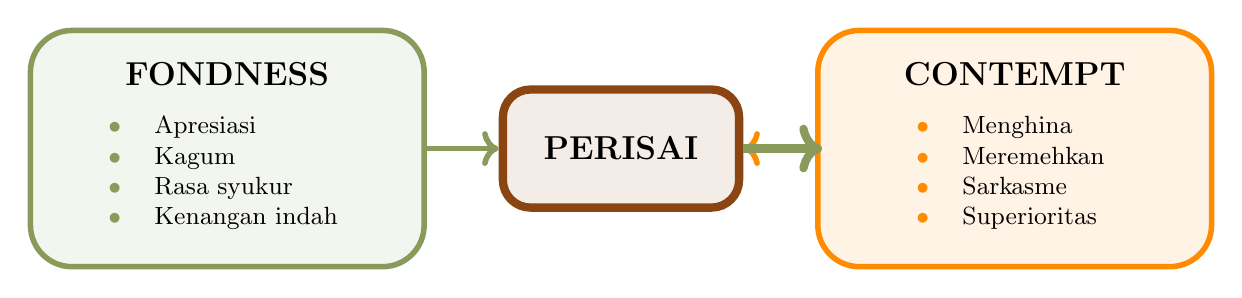
\begin{tikzpicture}[
    box/.style={draw=#1, line width=2pt, rounded corners=15pt,
                fill=#1!10, minimum width=5cm, minimum height=3cm, align=center}
]
    % Fondness Box
    \node[box=sagegreen] (fond) at (0,0) {
        \textbf{\large FONDNESS}\\[0.3cm]
        \small
        {\small
        \begin{tabular}{ll}
        \textcolor{sagegreen}{$\bullet$} & Apresiasi \\
        \textcolor{sagegreen}{$\bullet$} & Kagum \\
        \textcolor{sagegreen}{$\bullet$} & Rasa syukur \\
        \textcolor{sagegreen}{$\bullet$} & Kenangan indah \\
        \end{tabular}
        }
    };
    
    % Shield
    \node[draw=primary, line width=3pt, rounded corners=10pt,
          fill=primary!10, minimum width=3cm, minimum height=1.5cm] (shield) at (5,0) {
        \textbf{\large PERISAI}
    };
    
    % Contempt Box
    \node[box=accent] (cont) at (10,0) {
        \textbf{\large CONTEMPT}\\[0.3cm]
        \small
        {\small
        \begin{tabular}{ll}
        \textcolor{accent}{$\bullet$} & Menghina \\
        \textcolor{accent}{$\bullet$} & Meremehkan \\
        \textcolor{accent}{$\bullet$} & Sarkasme \\
        \textcolor{accent}{$\bullet$} & Superioritas \\
        \end{tabular}
        }
    };
    
    % Arrows
    \draw[->, line width=2pt, sagegreen] (fond) -- (shield);
    \draw[->, line width=2pt, accent] (cont) -- (shield);
    \draw[->, line width=3pt, sagegreen] (shield.east) -- ++(1,0);
\end{tikzpicture}
\end{center}

\section{Ilmu di Balik Fondness: Prediktor Stabilitas Hubungan}

\subsection{Penelitian Gottman yang Mengubah Segalanya}

Dalam penelitian longitudinal selama \textbf{16 tahun}, Gottman mengamati ribuan pasangan dan menemukan pola yang menakjubkan:

\begin{center}
\renewcommand{\arraystretch}{1.5}
\begin{tabular}{|>{\raggedright}p{4cm}|>{\raggedright}p{5cm}|>{\raggedright\arraybackslash}p{5cm}|}
\hline
\rowcolor{primary!20}
\textbf{Indikator} & \textbf{Pasangan Bahagia} & \textbf{Pasangan Tidak Bahagia} \\
\hline
Ekspresi fondness/hari & 5-20 kali & 0-2 kali \\
\hline
Rasio positif-negatif & 20:1 (konflik) & 0,8:1 \\
\hline
Kenangan masa awal & Hangat, detail & Dingin, kabur \\
\hline
Respons terhadap keberhasilan pasangan & Active Constructive & Passive/Destructive \\
\hline
\end{tabular}
\end{center}

\begin{insightbox}
\textbf{Fakta Mengejutkan:} Pasangan yang tetap bahagia selama 20+ tahun tidak memiliki \textit{lebih sedikit} konflik. Mereka hanya memiliki \highlight{lebih banyak fondness} yang melindungi hubungan saat konflik terjadi.
\end{insightbox}

\subsection{Neuroscience of Fondness}

Ketika kamu merasakan fondness:

\begin{enumerate}
    \item \textbf{Oxytocin naik} --- memperkuat ikatan emosional
    \item \textbf{Cortisol turun} --- mengurangi stres
    \item \textbf{Prefrontal cortex aktif} --- kemampuan regulasi emosi meningkat
    \item \textbf{Amygdala tenang} --- deteksi ``ancaman'' berkurang
\end{enumerate}

Ini menciptakan \keyterm{upward spiral} --- semakin kamu merasakan fondness, semakin mudah untuk melihat kebaikan pasangan.

\section{Mengapa Fondness Memudar?}

\subsection{Erosi Normal vs Penurunan Berbahaya}

\begin{warningbox}[Bedakan Dua Jenis Penurunan]
\textbf{Erosi Normal (Natural Decline):}
\begin{itemize}
    \item Terjadi perlahan selama 2-3 tahun pertama
    \item Fondness tetap ada, hanya frekuensi ungkapan berkurang
    \item Masih mudah mengingat hal-hal positif saat diminta
    \item Tidak ada rasa jengkel mendalam
\end{itemize}

\textbf{Penurunan Berbahaya (Dangerous Decline):}
\begin{itemize}
    \item Fondness digantikan oleh kritik berulang
    \item Sulit mengingat hal positif tentang pasangan
    \item Rasa jengkel muncul bahkan saat tidak ada masalah
    \item Kenangan masa lalu diceritakan dengan negatif
\end{itemize}
\end{warningbox}

\subsection{Faktor yang Mempercepat Hilangnya Fondness}

\begin{center}
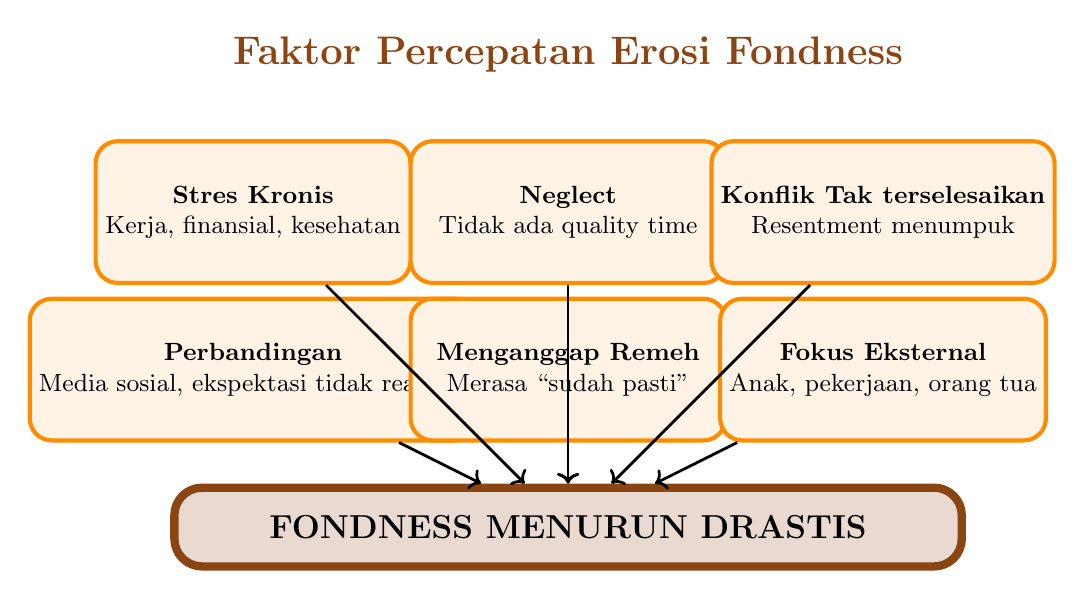
\begin{tikzpicture}[
    factor/.style={draw=accent, line width=1.5pt, rounded corners=8pt,
                   fill=accent!10, minimum width=4cm, minimum height=1.8cm,
                   align=center, font=\small}
]
    % Title
    \node[font=\Large\bfseries, primary] at (0,4) {Faktor Percepatan Erosi Fondness};
    
    % Factors
    \node[factor] (stress) at (-4,2) {\textbf{Stres Kronis}\\Kerja, finansial, kesehatan};
    \node[factor] (neglect) at (0,2) {\textbf{Neglect}\\Tidak ada quality time};
    \node[factor] (conflict) at (4,2) {\textbf{Konflik Tak terselesaikan}\\Resentment menumpuk};
    \node[factor] (comparison) at (-4,0) {\textbf{Perbandingan}\\Media sosial, ekspektasi tidak realistis};
    \node[factor] (taking) at (0,0) {\textbf{Menganggap Remeh}\\Merasa ``sudah pasti''};
    \node[factor] (external) at (4,0) {\textbf{Fokus Eksternal}\\Anak, pekerjaan, orang tua};
    
    % Arrow down
    \node[draw=primary, line width=3pt, rounded corners=10pt,
          fill=primary!20, minimum width=10cm, minimum height=1cm] (result) at (0,-2) {
        \textbf{\large FONDNESS MENURUN DRASTIS}
    };
    
    % Connecting lines
    \draw[->, line width=1pt] (stress) -- (result);
    \draw[->, line width=1pt] (neglect) -- (result);
    \draw[->, line width=1pt] (conflict) -- (result);
    \draw[->, line width=1pt] (comparison) -- (result);
    \draw[->, line width=1pt] (taking) -- (result);
    \draw[->, line width=1pt] (external) -- (result);
\end{tikzpicture}
\end{center}

\section{Self-Assessment: Mengukur Level Fondness-mu}

\begin{exercisebox}[Fondness Assessment Scale]
\textbf{Petunjuk:} Jawab setiap pertanyaan dengan skala 1-5:
\begin{itemize}
    \item[1] = Sangat tidak setuju
    \item[3] = Netral
    \item[5] = Sangat setuju
\end{itemize}

\subsection*{Bagian A: Ungkapan Fondness}

\begin{enumerate}
    \item Saya sering memuji pasangan saya secara spontan.
    \item Saya merasa bangga ketika menceritakan pasangan saya kepada orang lain.
    \item Saya menunjukkan kasih sayang fisik setiap hari (peluk, cium, gandeng tangan).
    \item Saya mengucapkan ``terima kasih'' atas hal-hal kecil yang pasangan lakukan.
    \item Saya sering tersenyum saat melihat/membayangkan pasangan saya.
\end{enumerate}

\subsection*{Bagian B: Pikiran dan Perasaan}

\begin{enumerate}
    \setcounter{enumi}{5}
    \item Ketika terpisah, saya sering memikirkan hal positif tentang pasangan.
    \item Saya merasa beruntung memiliki pasangan saya.
    \item Saya bisa dengan mudah menyebutkan 5 kualitas yang saya kagumi dari pasangan.
    \item Kenangan awal hubungan kami masih membawa perasaan hangat.
    \item Saya percaya pasangan saya adalah orang yang baik, meski punya kekurangan.
\end{enumerate}

\subsection*{Bagian C: Saat Konflik}

\begin{enumerate}
    \setcounter{enumi}{10}
    \item Saat marah, saya masih bisa mengingat hal-hal baik tentang pasangan.
    \item Saya menghindari menghina atau meremehkan pasangan saat bertengkar.
    \item Setelah konflik, saya bisa kembali merasa hangat pada pasangan.
    \item Saya tidak membuat kesalahan kecil menjadi masalah besar.
    \item Saya bisa memaafkan dan melupakan dengan relatif mudah.
\end{enumerate}

\subsection*{Scoring}

\begin{center}
\renewcommand{\arraystretch}{1.4}
\begin{tabular}{|c|c|l|}
\hline
\rowcolor{primary!20}
\textbf{Skor Total} & \textbf{Kategori} & \textbf{Interpretasi} \\
\hline
60-75 & \textcolor{sagegreen}{\textbf{Sangat Tinggi}} & Fondness system sangat kuat. Pertahankan! \\
\hline
45-59 & \textcolor{primary}{\textbf{Tinggi}} & Fondness baik, tapi ada ruang untuk ditingkatkan. \\
\hline
30-44 & \textcolor{accent}{\textbf{Sedang}} & Fondness mulai memudar. Perlu perhatian serius. \\
\hline
15-29 & \textcolor{red}{\textbf{Rendah}} & \textbf{Warning!} Fondness berbahaya. Butuh intervensi segera. \\
\hline
\end{tabular}
\end{center}
\end{exercisebox}

\section{Membangun Kembali Fondness: Proses Langkah demi Langkah}

\subsection{Untuk Pasangan yang Masih Memiliki Fondness}

\begin{tipbox}[Strategi Maintenance]
\begin{enumerate}
    \item \textbf{Buat Ritual Ungkapan}
    \begin{itemize}
        \item Setiap pagi: sebutkan 1 hal yang kamu hargai
        \item Setiap malam: ucapkan terima kasih untuk 1 hal spesifik hari ini
    \end{itemize}
    \item \textbf{Ciptakan Tradisi Positif}
    \begin{itemize}
        \item Anniversary celebration yang bermakna
        \item Weekly date night tanpa gadget
        \item Monthly reflection bersama
    \end{itemize}
    \item \textbf{Dokumentasikan Momen Bahagia}
    \begin{itemize}
        \item Foto album digital
        \item Journal kenangan bersama
        \item Box memorabilia
    \end{itemize}
\end{enumerate}
\end{tipbox}

\subsection{Untuk Pasangan yang Kehilangan Fondness}

\begin{warningbox}[Proses Rebuilding Butuh Waktu]
Membangun kembali fondness bukanlah proses instan. Dibutuhkan \textbf{6-12 bulan} konsistensi untuk mengembalikan sistem fondness yang kuat.
\end{warningbox}

\textbf{Langkah 1: Akui Masalahnya}
\begin{itemize}
    \item ``Aku sadar aku sudah lama tidak menunjukkan apresiasi padamu. Aku ingin mengubahnya.''
    \item Hindari defensive atau menyalahkan
    \item Terima bahwa ini butuh usaha dari kedua belah pihak
\end{itemize}

\textbf{Langkah 2: Mulai dengan Mengamati}
\begin{itemize}
    \item Luangkan 5 menit setiap hari untuk ``meneliti'' pasanganmu
    \item Catat hal-hal kecil yang dia lakukan dengan baik
    \item Perhatikan kualitas karakternya yang mungkin terlupakan
\end{itemize}

\textbf{Langkah 3: Ungkapkan Secara Bertahap}
\begin{itemize}
    \item Mulai dengan yang aman dan umum
    \item Tingkatkan spesifisitas dan frekuensi perlahan
    \item Jangan berharap respons positif langsung --- berikan waktu
\end{itemize}

\section{Praktik Harian: 20+ Tindakan Spesifik}

\subsection{Verbal Appreciations (Ungkapan Verbal)}

\begin{praktikbox}[Contoh Ungkapan Verbal]
\textbf{Tingkat 1 - Umum:}
\begin{itemize}
    \item ``Terima kasih ya.''
    \item ``Aku appreciate yang kamu lakukan.''
    \item ``Kamu hebat.''
\end{itemize}

\textbf{Tingkat 2 - Spesifik:}
\begin{itemize}
    \item ``Terima kasih sudah membuatkan kopi pagi ini. Aku butuh itu.''
    \item ``Aku notice kamu sudah bekerja keras minggu ini. Aku bangga padamu.''
    \item ``Cara kamu menangani situasi tadi sangat bijaksana.''
\end{itemize}

\textbf{Tingkat 3 - Mendalam:}
\begin{itemize}
    \item ``Aku bersyukur setiap hari karena kamu adalah pasanganku.''
    \item ``Kualitas kepedulianmu adalah hal yang paling aku kagumi dari dirimu.''
    \item ``Aku jadi orang yang lebih baik karena kamu ada di hidupku.''
\end{itemize}
\end{praktikbox}

\subsection{Affection Fisik}

\begin{center}
\renewcommand{\arraystretch}{1.4}
\begin{tabular}{|>{\raggedright}p{3cm}|>{\raggedright}p{4.5cm}|>{\raggedright\arraybackslash}p{6cm}|}
\hline
\rowcolor{sagegreen!20}
\textbf{Jenis Sentuhan} & \textbf{Contoh} & \textbf{Kapan Menggunakannya} \\
\hline
Micro-affection & Tap punggung, squeeze tangan, touch shoulder & Saat lewat, saat bekerja sama, saat berpisah \\
\hline
Greeting affection & Peluk saat pulang, cium dahi & Setiap kali bertemu setelah terpisah \\
\hline
Comforting touch & Peluk lama, gosok punggung & Saat pasangan stres, sedih, atau capek \\
\hline
Playful touch & Bercanda, bergandengan jalan & Saat santai, jalan-jalan, momen ringan \\
\hline
Intimate touch & Ciuman, berpelukan tanpa agenda & Saat quality time, sebelum tidur \\
\hline
\end{tabular}
\end{center}

\subsection{Acts of Service (Tindakan Pelayanan)}

\begin{enumerate}
    \item \textbf{Morning routine support:} Siapkan sarapan atau kopi
    \item \textbf{Evening wind-down:} Urut bahu pasangan setelah hari yang panjang
    \item \textbf{Task takeover:} Ambil alih tugas yang biasanya pasangan lakukan
    \item \textbf{Proactive help:} Lihat apa yang butuh dikerjakan dan lakukan tanpa diminta
    \item \textbf{Comfort creation:} Siapkan mandi hangat, nyalakan lilin, atmosfer nyaman
\end{enumerate}

\subsection{Quality Time}

\begin{tipbox}[Ide Quality Time 15-30 Menit]
\begin{itemize}
    \item[$\bullet$] \textbf{Morning check-in:} Duduk bersama sambil minum kopi, bicara rencana hari
    \item[$\bullet$] \textbf{Evening debrief:} Ceritakan satu hal baik dan satu tantangan dari hari ini
    \item[$\bullet$] \textbf{Walk together:} Jalan sore sambil bergandengan
    \item[$\bullet$] \textbf{Cook together:} Masak bersama sambil bercanda
    \item[$\bullet$] \textbf{Tech-free time:} Duduk berhadapan tanpa gadget selama 20 menit
\end{itemize}
\end{tipbox}

\subsection{Small Gestures (Hadiah Kecil)}

\begin{enumerate}
    \item Catatan singkat di tempat tak terduga (kotak bekal, cermin kamar mandi)
    \item Membeli makanan favoritnya saat pulang kerja
    \item Kirim pesan singkat di tengah hari: ``Lagi mikirin kamu."
    \item Ambilkan benda yang dia butuhkan tanpa diminta
    \item Buat playlist lagu yang mengingatkan padanya
    \item Foto momen kecil dan kirim dengan caption manis
    \item Siapkan ``emergency kit'' di mobil: makanan favorit, obat, tissue
\end{enumerate}

\section{The 7-Week Fondness Exercise: Rencana Mingguan}

\begin{exercisebox}[Program 7 Minggu Transformasi]
\renewcommand{\arraystretch}{1.6}
\begin{tabular}{|c|>{\raggedright}p{4cm}|>{\raggedright\arraybackslash}p{7cm}|}
\hline
\rowcolor{primary!20}
\textbf{Minggu} & \textbf{Fokus} & \textbf{Tugas Harian} \\
\hline
1 & \textbf{Apresiasi Dasar} & Ucapkan 1 hal spesifik yang kamu hargai setiap hari \\
\hline
2 & \textbf{Kenangan Indah} & Ceritakan ulang 1 kenangan indah masa pacaran/dating \\
\hline
3 & \textbf{Kualitas Kagum} & Identifikasi dan ucapkan 1 kualitas karakter yang kamu kagumi \\
\hline
4 & \textbf{Mikro-Momen} & Ciptakan 3 micro-momen koneksi (sentuhan, eye contact, senyum) \\
\hline
5 & \textbf{Public Pride} & Ungkapkan kebanggaan pada pasangan di depan orang lain 1x \\
\hline
6 & \textbf{Love Notes} & Tulis catatan singkat/manis yang ditinggalkan di tempat tak terduga \\
\hline
7 & \textbf{Integrasi} & Lakukan semua praktik minggu 1-6 setiap hari \\
\hline
\end{tabular}

\vspace{0.5cm}
\textbf{Tips Keberhasilan:}
\begin{itemize}
    \item Jadwalkan waktu yang sama setiap hari (misal: saat sarapan dan sebelum tidur)
    \item Gunakan reminder di HP untuk 30 hari pertama
    \item Buat journal tracking untuk mencatat progress
    \item Rayakan milestone bersama setiap minggu
\end{itemize}
\end{exercisebox}

\section{Mengungkapkan Admiration dengan Efektif}

\subsection{Specific vs Generic Compliments}

\begin{warningbox}[Hindari Pujian Generik]
Pujian seperti ``Kamu baik'' atau ``Kamu cantik/ganteng'' memiliki dampak terbatas karena:
\begin{itemize}
    \item Terlalu umum --- bisa diucapkan ke siapa saja
    \item Tidak menunjukkan bahwa kamu benar-benar \textit{melihat} pasanganmu
    \item Mudah dilupakan
\end{itemize}
\end{warningbox}

\begin{praktikbox}[Formula Pujian Spesifik]
\textbf{Template:} ``Aku [perasaan] ketika kamu [tindakan spesifik] karena [dampak/makna].''

\textbf{Contoh:}
\begin{itemize}
    \item ``Aku \textbf{merasa dihargai} ketika kamu \textbf{menanyakan hari ku hari ini} karena \textbf{itu menunjukkan kamu peduli dengan apa yang kulakukan}.''
    \item ``Aku \textbf{bangga} melihat cara kamu \textbf{menangani deadline yang ketat minggu ini} karena \textbf{kamu tetap tenang dan profesional}.''
    \item ``Aku \textbf{terkesan} dengan \textbf{kesabaranmu saat mengajari anak belajar} karena \textbf{kamu menjelaskan dengan lembut meski capek}.''
\end{itemize}
\end{praktikbox}

\subsection{The 5:1 Ratio dalam Action}

Gottman menemukan bahwa pasangan bahagia memiliki rasio \textbf{5 interaksi positif : 1 interaksi negatif} saat konflik.

\begin{center}
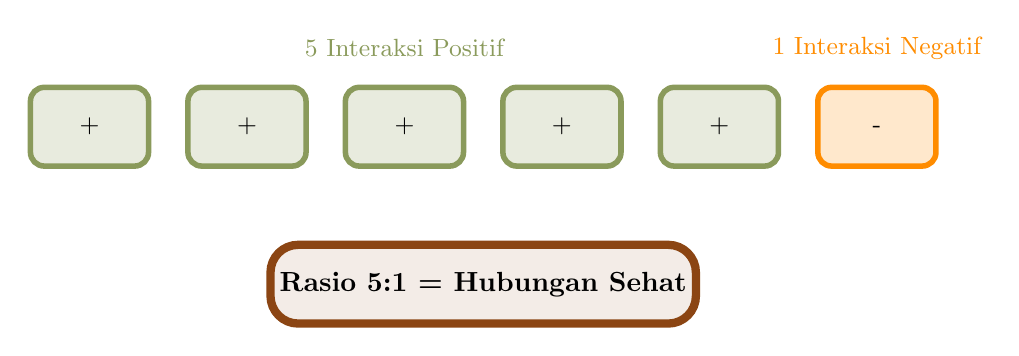
\begin{tikzpicture}[
    posbox/.style={draw=sagegreen, line width=2pt, rounded corners=5pt,
                fill=sagegreen!20, minimum width=1.5cm, minimum height=1cm, font=\small},
    negbox/.style={draw=accent, line width=2pt, rounded corners=5pt,
                fill=accent!20, minimum width=1.5cm, minimum height=1cm, font=\small}
]
    % 5 positive boxes
    \node[posbox] (p1) at (0,0) {+};
    \node[posbox] (p2) at (2,0) {+};
    \node[posbox] (p3) at (4,0) {+};
    \node[posbox] (p4) at (6,0) {+};
    \node[posbox] (p5) at (8,0) {+};
    \node[negbox] (n1) at (10,0) {-};
    
    % Label
    \node[font=\small, sagegreen] at (4,1) {5 Interaksi Positif};
    \node[font=\small, accent] at (10,1) {1 Interaksi Negatif};
    
    % Ratio
    \node[draw=primary, line width=3pt, rounded corners=10pt,
          fill=primary!10, minimum width=4cm, minimum height=1cm] at (5,-2) {
        \textbf{Rasio 5:1 = Hubungan Sehat}
    };
\end{tikzpicture}
\end{center}

\section{Menerima Admiration dengan Grace}

\subsection{Kenapa Sulit Menerima Pujian?}

Banyak orang merasa \textbf{tidak nyaman} saat dipuji karena:
\begin{itemize}
    \item \textbf{Low self-esteem:} Merasa tidak pantas dipuji
    \item \textbf{Fear of expectations:} Takut harus mempertahankan standar
    \item \textbf{Cultural conditioning:} Dibiasakan untuk merendah
    \item \textbf{Distrust:} Meragukan kejujuran pujian
\end{itemize}

\subsection{Cara Menerima dengan Baik}

\begin{tipbox}[Respons yang Membangun]
\textbf{Lakukan:}
\begin{enumerate}
    \item \textbf{Terima dengan sederhana:} ``Terima kasih, aku appreciate pujianmu.''
    \item \textbf{Akui usaha:} ``Aku memang berusaha keras untuk itu.''
    \item \textbf{Bagikan credit:} ``Aku belajar banyak dari kamu juga.''
    \item \textbf{Reflect back:} ``Itu berarti banyak dari kamu.''
\end{enumerate}

\textbf{Hindari:}
\begin{itemize}
    \item Menyangkal: ``Ah, enggak kok, biasa aja.''
    \item Defleksi: ``Bajuku aja yang bagus.''
    \item Counter-criticism: ``Tapi aku jelek di hal lain.''
    \item Silence awkward: Diam saja tanpa respons
\end{itemize}
\end{tipbox}

\section{Menjaga Fondness Saat Konflik}

\subsection{Softened Start-up dengan Fondness}

Saat membahas masalah sulit, mulailah dengan fondness:

\begin{center}
\renewcommand{\arraystretch}{1.5}
\begin{tabular}{|>{\raggedright}p{6cm}|>{\raggedright\arraybackslash}p{8cm}|}
\hline
\rowcolor{accent!20}
\textbf{Hard Start-up (Negatif)} & \textbf{Softened Start-up (Dengan Fondness)} \\
\hline
``Kamu selalu lupa membuang sampah!'' & ``Aku tahu kamu sibuk, tapi aku butuh bantuan dengan sampah.'' \\
\hline
``Kamu nggak pernah dengerin aku!'' & ``Aku tahu kamu care, tapi saat ini aku butuh full attention-mu.'' \\
\hline
``Kamu egois banget sih!'' & ``Biasanya kamu very considerate, tapi keputusan ini bikin aku kecewa.'' \\
\hline
\end{tabular}
\end{center}

\subsection{Repair Attempts yang Efektif}

\begin{praktikbox}[Repair Attempts dengan Fondness]
\textbf{Phrase untuk mengembalikan fondness saat konflik:}
\begin{itemize}
    \item ``Aku tahu kita bisa lewati ini. Aku di sini.''
    \item ``Ini bukan tentang kita melawan satu sama lain, tapi kita vs masalah ini.''
    \item ``Aku marah, tapi aku tetap cinta kamu.''
    \item ``Aku appreciate kamu masih mau bicara tentang ini.''
    \item ``Maaf, aku salah. Kamu pantas mendapatkan pendengaran yang lebih baik.''
\end{itemize}
\end{praktikbox}

\section{Integrasi dengan Attachment Styles}

\begin{insightbox}
Setiap attachment style memiliki cara unik dalam memberikan dan menerima fondness. Memahami ini membantu pasangan saling memenuhi kebutuhan emosional dengan lebih efektif.
\end{insightbox}

\subsection{Tabel Integrasi Lengkap}

\begin{center}
\renewcommand{\arraystretch}{1.6}
\begin{tabular}{|>{\raggedright}p{2.5cm}|>{\raggedright}p{4cm}|>{\raggedright}p{4cm}|>{\raggedright\arraybackslash}p{4cm}|}
\hline
\rowcolor{primary!20}
\textbf{Attachment} & \textbf{Cara Memberi Fondness} & \textbf{Cara Menerima Fondness} & \textbf{Kebutuhan Spesifik} \\
\hline
\textbf{Anchor} & Natural dan berimbang; verbal, fisik, service dengan mudah & Nyaman dan menerima dengan terbuka & Konsistensi dan kualitas waktu \\
\hline
\textbf{Island} & Melalui acts of service lebih dari verbal; menunjukkan dengan tindakan & Sulit menerima verbal, lebih nyaman dengan non-verbal & Jangan terlalu ``tebal'', beri ruang \\
\hline
\textbf{Wave} & Generous dan banyak; verbal dan fisik melimpah & Butuh validasi berulang, takut pujian palsu & Reassurance dan konsistensi \\
\hline
\end{tabular}
\end{center}

\subsection{Strategi untuk Setiap Kombinasi}

\begin{tipbox}[Panduan Berdasarkan Kombinasi]
\textbf{Anchor + Island:}
\begin{itemize}
    \item Anchor: Hargai cara non-verbal Island menunjukkan cinta
    \item Island: Latih diri untuk menerima dan merespons verbal affection
\end{itemize}

\textbf{Anchor + Wave:}
\begin{itemize}
    \item Anchor: Berikan reassurance ekstra tanpa merasa ``cukup sudah''
    \item Wave: Terima bahwa Anchor tidak perlu ``diuji'' terus-menerus
\end{itemize}

\textbf{Island + Wave:}
\begin{itemize}
    \item Island: Berusaha lebih ekspresif meski tidak nyaman
    \item Wave: Beri ruang saat Island perlu withdraw, jangan personalisasi
\end{itemize}
\end{tipbox}

\section{Studi Kasus: Rebuilding dari Nol}

\subsection{Kasus 1: David dan Sarah (15 Tahun Menikah)}

\begin{insightbox}
\textbf{Situasi:} David dan Sarah hampir bercerai. David merasa Sarah ``tidak pernah puas'', Sarah merasa David ``tidak peduli''. Fondness hampir nol --- mereka tidak pernah memuji satu sama lain selama 3 tahun terakhir.

\textbf{Intervensi:}
\begin{enumerate}
    \item \textbf{Minggu 1-2:} Mereka hanya diminta untuk \textit{mencatat} 1 hal positif tentang pasangan setiap hari, tanpa mengungkapkan.
    \item \textbf{Minggu 3-4:} Mulai mengungkapkan 1 apresiasi sederhana setiap hari.
    \item \textbf{Minggu 5-6:} Share kenangan indah dari 15 tahun pernikahan.
    \item \textbf{Minggu 7-8:} Weekly date night dengan tema ``apresiasi''.
\end{enumerate}

\textbf{Hasil:} Setelah 6 bulan, mereka melaporkan ``jatuh cinta lagi''. David belajar melihat usaha Sarah yang dia anggap ``mengeluh'' sebenarnya adalah kepedulian. Sarah belajar melihat ketenangan David bukan ``tidak peduli'' tapi ``stabilitas''.
\end{insightbox}

\subsection{Kasus 2: Mike dan Lisa (Island + Wave Dynamic)}

\begin{insightbox}
\textbf{Situasi:} Mike (Island) dan Lisa (Wave) dalam spiral negatif. Lisa mendesak affection, Mike semakin menjauh. Lisa merasa tidak dicintai, Mike merasa tidak cukup baik.

\textbf{Strategi Khusus:}
\begin{itemize}
    \item Mike diajari ``micro-affection'' --- sentuhan kecil yang tidak membuatnya overwhelm
    \item Lisa diajari ``receive without pursuit'' --- menerima affection tanpa langsung menuntut lebih
    \item Mereka membuat ``affection schedule'' yang bisa diprediksi
\end{itemize}

\textbf{Breakthrough:} Ketika Lisa berhenti mengejar, Mike justru mulai mendekat. Ketika Mike memberi affection tanpa diminta, Lisa merasa aman.
\end{insightbox}

\section{30-Day Fondness Challenge}

\begin{exercisebox}[Tantangan 30 Hari: Prompt Harian]
\textbf{Instruksi:} Setiap hari, gunakan prompt berikut untuk mengungkapkan fondness pada pasangan. Variasikan cara ungkapannya (verbal, catatan, tindakan).

\renewcommand{\arraystretch}{1.4}
\begin{tabular}{|c|>{\raggedright\arraybackslash}p{10cm}|}
\hline
\rowcolor{primary!20}
\textbf{Hari} & \textbf{Prompt} \\
\hline
1 & Sebutkan 1 hal yang pasanganmu lakukan hari ini yang kamu hargai. \\
\hline
2 & Ceritakan kenangan pertama kalian dengan detail. \\
\hline
3 & Apa 1 kualitas karakter pasanganmu yang kamu kagumi? \\
\hline
4 & Ucapkan terima kasih untuk hal kecil yang sering dianggap remeh. \\
\hline
5 & Peluk pasanganmu selama 20 detik tanpa bicara. \\
\hline
6 & Tulis catatan singkat dan sembunyikan di tempat tak terduga. \\
\hline
7 & Ceritakan pada orang lain (di depan pasanganmu) hal baik tentangnya. \\
\hline
8 & Lakukan 1 tugas yang biasanya pasanganmu kerjakan. \\
\hline
9 & Sebutkan 3 hal yang membuatmu tertawa bersamanya. \\
\hline
10 & Buat playlist lagu yang mengingatkan padanya. \\
\hline
11 & Berikan komplimen spesifik tentang penampilannya hari ini. \\
\hline
12 & Ceritakan momen saat kamu paling bangga padanya. \\
\hline
13 & Kirim pesan singkat di tengah hari: ``Sedang mikirin kamu.'' \\
\hline
14 & Lakukan aktivitas favoritnya meski bukan favoritmu. \\
\hline
15 & Sebutkan 1 hal yang kamu pelajari darinya. \\
\hline
\end{tabular}
\end{exercisebox}

\begin{exercisebox}[Tantangan 30 Hari: Lanjutan]
\renewcommand{\arraystretch}{1.4}
\begin{tabular}{|c|>{\raggedright\arraybackslash}p{10cm}|}
\hline
\rowcolor{primary!20}
\textbf{Hari} & \textbf{Prompt} \\
\hline
16 & Buat daftar 10 hal yang kamu syukuri tentang pernikahan/hubunganmu. \\
\hline
17 & Berikan massage sederhana di bahu atau punggung. \\
\hline
18 & Ceritakan kenangan lucu yang melibatkan kalian berdua. \\
\hline
19 & Ucapkan ``Aku cinta kamu'' dengan cara yang berbeda dari biasanya. \\
\hline
20 & Siapkan makanan favoritnya sebagai kejutan. \\
\hline
21 & Sebutkan 1 mimpi/karir goal-nya dan dukung secara verbal. \\
\hline
22 & Tulis surat singkat (setengah halaman) tentang kenapa kamu bersyukur. \\
\hline
23 & Lakukan eye contact selama 2 menit tanpa bicara. \\
\hline
24 & Berikan hadiah kecil tanpa alasan khusus. \\
\hline
25 & Ceritakan bagaimana pasanganmu telah membantumu tumbuh. \\
\hline
26 & Ucapkan maaf untuk hal kecil yang mungkin menyakitinya. \\
\hline
27 & Buat ritual selamat datang saat dia pulang dengan affection. \\
\hline
28 & Sebutkan 1 hal yang kamu nantikan tentang masa depan bersama. \\
\hline
29 & Lakukan ``debriefing positif'': ceritakan 1 hal baik dari minggu ini. \\
\hline
30 \textbf{*} & Rayakan completion dengan date night dan reflection bersama. \\
\hline
\end{tabular}

\vspace{0.5cm}
\textit{* Hari 30: Buat commitment untuk melanjutkan minimal 3 praktik yang paling berdampak.}
\end{exercisebox}

\section{Ringkasan dan Action Steps}

\begin{insightbox}
\textbf{Key Takeaways:}
\begin{enumerate}
    \item \highlight{Fondness adalah fondasi} --- tanpanya, konflik akan menghancurkan hubungan.
    \item Fondness bisa \highlight{dibangun kembali} meski hilang selama bertahun-tahun.
    \item Konsistensi lebih penting daripada grand gestures.
    \item Setiap attachment style memiliki bahasa fondness yang berbeda.
    \item Fondness harus diungkapkan \textbf{setiap hari}, bukan hanya saat senang.
\end{enumerate}
\end{insightbox}

\subsection{Action Plan untuk 7 Hari ke Depan}

\begin{exercisebox}[Langkah Langsung]
\textbf{Hari Ini:}
\begin{itemize}
    \item Kerjakan Fondness Assessment Scale
    \item Diskusikan hasil dengan pasangan
\end{itemize}

\textbf{Besok:}
\begin{itemize}
    \item Mulai dengan 1 apresiasi verbal spesifik
    \item Ciptakan 1 micro-moment affection
\end{itemize}

\textbf{Minggu Ini:}
\begin{itemize}
    \item Pilih 3 praktik dari 20+ tindakan yang akan dilakukan setiap hari
    \item Set reminder untuk consistency
    \item Mulai 30-Day Challenge
\end{itemize}

\textbf{Minggu Depan:}
\begin{itemize}
    \item Review: Apa yang berhasil? Apa yang perlu disesuaikan?
    \item Naikkan tingkat kesulitan/depth dari ungkapan
    \item Jadwalkan quality time khusus
\end{itemize}
\end{exercisebox}

\begin{tipbox}[Mantra Harian]
\begin{center}
\Large
``\textit{Hari ini, aku akan mencari dan mengungkapkan\\
setidaknya satu hal yang aku hargai dari pasanganku.}''
\end{center}
\end{tipbox}

\chapter{Menciptakan Makna Bersama: Shared Meaning System}

\begin{insightbox}
\textit{``Hubungan yang benar-benar sukses bukan hanya tentang bertahan dari konflik atau membangun keintiman harian. Puncaknya adalah ketika kalian menciptakan \highlight{makna bersama}---sebuah budaya hubungan yang unik, ritual yang mengikat, dan tujuan hidup yang dibangun berdua. Ini adalah Prinsip 7: cita-cita tertinggi dari hubungan yang berkembang.''} --- Dr. John Gottman
\end{insightbox}

\section{Apa itu Shared Meaning?}

\keyterm{Shared meaning} adalah sistem nilai, simbol, dan tujuan bersama yang menciptakan identitas unik bagi sebuah hubungan. Ini melampaui sekadar menjalani hari demi hari---ini tentang \highlight{kehidupan bersama dengan tujuan}.

\begin{praktikbox}[Definisi Shared Meaning yang Mendalam]
Shared meaning terdiri dari empat pilar utama:

\begin{enumerate}
    \item \textbf{Rituals of Connection:} Tradisi dan rutinitas yang mengikat
    \item \textbf{Roles:} Makna dari menjadi ``suami/istri/pasangan''
    \item \textbf{Goals:} Impian dan tujuan hidup yang dibangun bersama
    \item \textbf{Symbols:} Arti dari rumah, uang, waktu, dan objek bersama
\end{enumerate}

\textit{Shared meaning bukan sekadar kesamaan---ini tentang saling menghormati perbedaan sambil menciptakan kehidupan yang bermakna bersama.}
\end{praktikbox}

\subsection{Shared Meaning vs Daily Logistics}

Banyak pasangan mengira mereka punya shared meaning hanya karena mereka:
\begin{itemize}
    \item Hidup di rumah yang sama
    \item Membagi tugas rumah tangga
    \item Mengurus anak bersama
    \item Membayar tagihan bersama
\end{itemize}

\begin{warningbox}[Perbedaan Fundamental]
\textbf{Daily Logistics (Operasional):}
\begin{itemize}
    \item ``Siapa yang ambil anak hari ini?''
    \item ``Berapa budget bulan ini?''
    \item ``Acara keluarga minggu depan kita pergi?''
\end{itemize}

\textbf{Shared Meaning (Filosofis):}
\begin{itemize}
    \item ``Apa makna menjadi orang tua bagi kita?''
    \item ``Bagaimana uang mencerminkan nilai kita?''
    \item ``Tradisi keluarga apa yang ingin kita bangun?''
\end{itemize}

\textit{Pasangan dengan shared meaning kuat menjalani \textbf{kehidupan yang sama}. Pasangan tanpa shared meaning hanya \textbf{hidup berdampingan}.}
\end{warningbox}

\section{The Culture of Relationship: Membangun Budaya Hubungan}

Setiap hubungan memiliki \keyterm{budaya}---serangkaian aturan tak tertulis, nilai, dan praktik yang mengatur bagaimana pasangan hidup bersama. Budaya ini bisa dibangun dengan sengaja atau terbentuk secara tak sadar.

\begin{center}
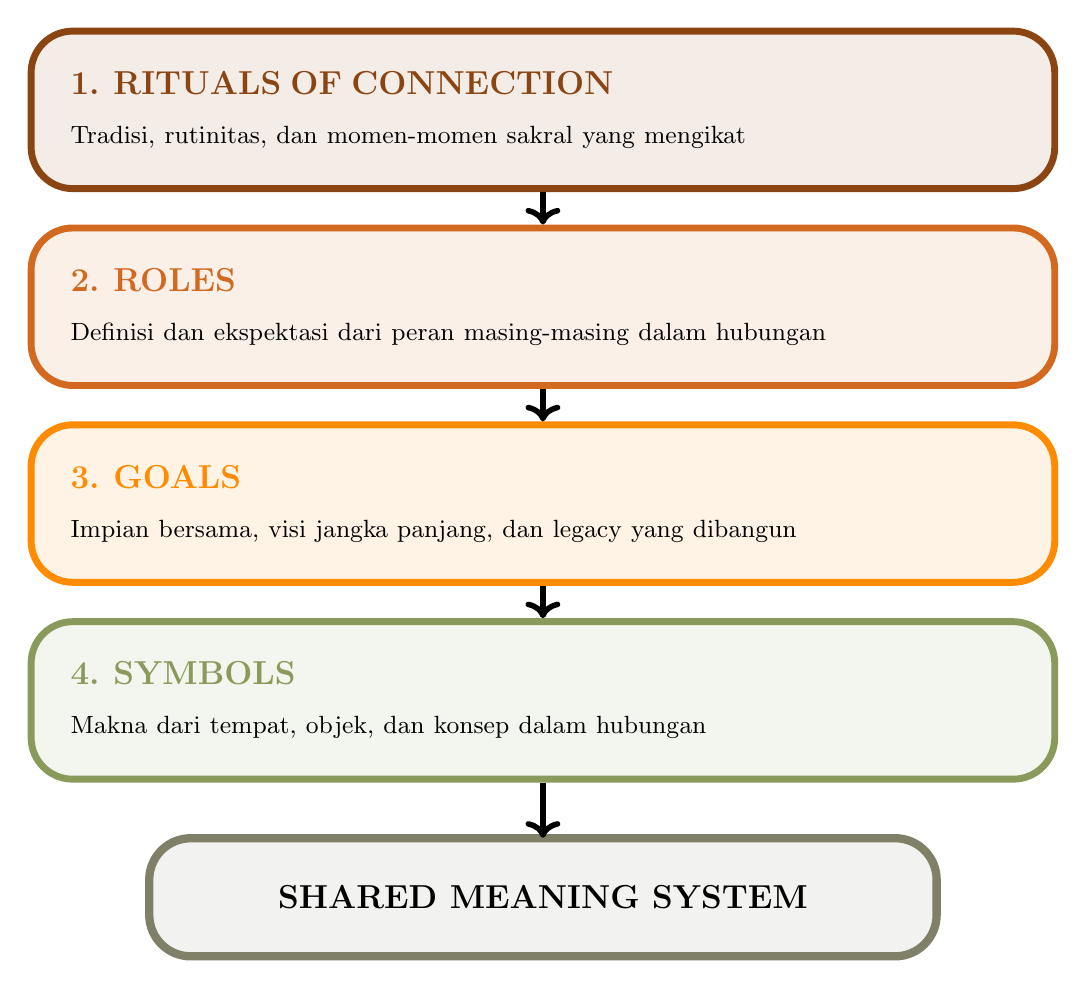
\begin{tikzpicture}[
    culture/.style={draw=#1, line width=2.5pt, rounded corners=15pt,
                    fill=#1!10, minimum width=13cm, minimum height=2cm,
                    align=left, text width=12cm}
]
    \node[culture=primary] (ritual) at (0,6) {
        \textbf{\large \textcolor{primary}{1. RITUALS OF CONNECTION}}\\[0.2cm]
        \small Tradisi, rutinitas, dan momen-momen sakral yang mengikat
    };
    
    \node[culture=secondary] (roles) at (0,3.5) {
        \textbf{\large \textcolor{secondary}{2. ROLES}}\\[0.2cm]
        \small Definisi dan ekspektasi dari peran masing-masing dalam hubungan
    };
    
    \node[culture=accent] (goals) at (0,1) {
        \textbf{\large \textcolor{accent}{3. GOALS}}\\[0.2cm]
        \small Impian bersama, visi jangka panjang, dan legacy yang dibangun
    };
    
    \node[culture=sagegreen] (symbols) at (0,-1.5) {
        \textbf{\large \textcolor{sagegreen}{4. SYMBOLS}}\\[0.2cm]
        \small Makna dari tempat, objek, dan konsep dalam hubungan
    };
    
    \node[draw=warmgray, line width=3pt, rounded corners=15pt, 
          fill=warmgray!10, minimum width=10cm, minimum height=1.5cm, align=center] 
          at (0,-4) {\textbf{\large SHARED MEANING SYSTEM}};
    
    \draw[->, line width=2pt] (ritual.south) -- (roles.north);
    \draw[->, line width=2pt] (roles.south) -- (goals.north);
    \draw[->, line width=2pt] (goals.south) -- (symbols.north);
    \draw[->, line width=2pt] (symbols.south) -- ++(0,-0.7);
\end{tikzpicture}
\end{center}

\subsection{Mengapa Budaya Hubungan Penting?}

\begin{praktikbox}[Benefit Shared Meaning System]
\textbf{1. Sense of Unity}
\begin{itemize}
    \item ``Kita'' menjadi lebih penting dari ``Aku'' vs ``Kamu''
    \item Identitas sebagai tim terbentuk
    \item Loyalitas pada hubungan meningkat
\end{itemize}

\textbf{2. Resilience During Stress}
\begin{itemize}
    \item Ritual menjadi anchor saat krisis
    \item Nilai bersama memberi arah dalam keputusan sulit
    \item Shared meaning sebagai ``why'' yang memotivasi bertahan
\end{itemize}

\textbf{3. Protection Against Drift}
\begin{itemize}
    \item Mencegah hubungan menjadi ``roommate arrangement''
    \item Menjaga romance di tengah rutinitas
    \item Memberi makna pada usaha-usaha kecil sehari-hari
\end{itemize}
\end{praktikbox}

\section{Self-Assessment: Seberapa Kuat Shared Meaning-mu?}

\begin{exercisebox}[Shared Meaning Assessment]
\textbf{Petunjuk:} Jawab setiap pertanyaan dengan skala 1-5 (1 = Sangat tidak setuju, 5 = Sangat setuju)

\subsection*{BAGIAN A: Rituals (1-5 poin per item)}
\begin{enumerate}
    \item Kami memiliki rutinitas pagi yang konsisten bersama
    \item Kami punya tradisi akhir pekan yang kami nantikan
    \item Ada ritual khusus saat kami berpisah dan bertemu kembali
    \item Kami merayakan anniversary dengan cara yang bermakna
    \item Ada ritual sebelum tidur yang menguatkan koneksi kami
    \item Kami punya tradisi liburan tahunan yang konsisten
\end{enumerate}

\subsection*{BAGIAN B: Roles (1-5 poin per item)}
\begin{enumerate}
    \item[7.] Kami sepakat tentang makna ``suami'' dan ``istri'' dalam hubungan kami
    \item[8.] Peran kami sebagai orang tua (jika ada anak) sejalan dengan nilai kami
    \item[9.] Kami jelas tentang ekspektasi satu sama lain dalam rumah tangga
    \item[10.] Kami merasa bangga dengan peran kami masing-masing
    \item[11.] Ada pembagian tanggung jawab yang fair dan disepakati
\end{enumerate}

\subsection*{BAGIAN C: Goals (1-5 poin per item)}
\begin{enumerate}
    \item[12.] Kami punya visi jangka panjang yang sama tentang masa depan
    \item[13.] Kami sering mendiskusikan impian dan aspirasi hidup
    \item[14.] Tujuan karir/finansial kami saling mendukung
    \item[15.] Kami punya proyek bersama yang sedang dikerjakan
    \item[16.] Legacy apa yang ingin kami tinggalkan sudah jelas
\end{enumerate}

\subsection*{BAGIAN D: Symbols (1-5 poin per item)}
\begin{enumerate}
    \item[17.] Rumah kami mencerminkan nilai dan identitas kami berdua
    \item[18.] Kami setuju tentang makna uang dalam hidup kami
    \item[19.] Waktu bersama dihargai sebagai komoditas yang berharga
    \item[20.] Ada objek/ruang khusus yang punya makna simbolis bagi kami
\end{enumerate}

\vspace{0.5cm}
\textbf{SCORING:}

\begin{center}
\renewcommand{\arraystretch}{1.4}
\begin{tabular}{|c|c|p{7cm}|}
\hline
\rowcolor{primary!20}
\textbf{Skor Total} & \textbf{Level} & \textbf{Interpretasi} \\
\hline
80-100 & \textbf{Sangat Kuat} & Shared meaning system sangat terbentuk. Hubungan punya fondasi filosofis yang kokoh \\
\hline
60-79 & \textbf{Kuat} & Ada fondasi yang baik, tapi masih ada area untuk ditingkatkan \\
\hline
40-59 & \textbf{Sedang} & Shared meaning mulai terbentuk tapi belum solid. Perlu sengaja membangun \\
\hline
20-39 & \textbf{Lemah} & Shared meaning minim. Risiko drift dan kehampaan hubungan \\
\hline
\textless 20 & \textbf{Sangat Lemah} & Shared meaning hampir tidak ada. Intervensi segera diperlukan \\
\hline
\end{tabular}
\end{center}
\end{exercisebox}

\section{Level 1: Rituals of Connection}

\keyterm{Rituals} adalah tindakan yang diulang dengan makna simbolis---bukan sekadar kebiasaan, tapi praktik yang sengaja dibangun untuk memperkuat ikatan.

\subsection{Jenis-Jenis Ritual}

\begin{center}
\renewcommand{\arraystretch}{1.5}
\begin{tabular}{|>{\raggedright}p{2.5cm}|>{\raggedright}p{4.5cm}|>{\raggedright}p{4.5cm}|>{\raggedright\arraybackslash}p{3.5cm}|}
\hline
\rowcolor{primary!20}
\textbf{Frekuensi} & \textbf{Contoh Ritual} & \textbf{Fungsi} & \textbf{Pentingnya} \\
\hline
\textbf{Daily} & Morning coffee together, Goodbye kiss, Dinner ritual, Bedtime routine & Menjaga koneksi harian & \textcolor{sagegreen}{Sangat Tinggi} \\
\hline
\textbf{Weekly} & Date night, Sunday brunch, Weekend walk & Recharge dan quality time & \textcolor{sagegreen}{Tinggi} \\
\hline
\textbf{Monthly} & Relationship check-in, Adventure day, Financial review & Maintenance dan planning & \textcolor{secondary}{Sedang} \\
\hline
\textbf{Annual} & Anniversary celebration, Vacation ritual, Year-end reflection & Milestone dan renewal & \textcolor{secondary}{Sedang} \\
\hline
\textbf{Life Events} & Birth rituals, Career celebration, Grieving together & Transisi hidup & \textcolor{sagegreen}{Sangat Tinggi} \\
\hline
\end{tabular}
\end{center}

\subsection{Membangun Ritual dari Nol}

\begin{tipbox}[Panduan Membangun Ritual Baru]
\textbf{Step 1: Identifikasi Gap}
\begin{itemize}
    \item Kapan kalian merasa paling terhubung?
    \item Kapan kalian merasa paling terpisah?
    \item Apa ritual dari masa kecil yang ingin kalian lanjutkan atau hindari?
\end{itemize}

\textbf{Step 2: Desain Ritual}
\begin{itemize}
    \item Pilih waktu yang konsisten
    \item Tentukan struktur (apa yang terjadi, dalam urutan apa)
    \item Buat elemen simbolis (objek, lagu, frasa khusus)
\end{itemize}

\textbf{Step 3: Implementasi}
\begin{itemize}
    \item Mulai sederhana---jangan terlalu kompleks
    \item Konsisten selama 21 hari untuk membentuk kebiasaan
    \item Evaluasi dan adjust setelah sebulan
\end{itemize}

\textbf{Step 4: Proteksi}
\begin{itemize}
    \item Jadikan ritual ``sacred''---prioritas non-negotiable
    \item Komunikasikan pada orang lain (anak, kerjaan) bahwa ini penting
    \item Jaga ritual bahkan saat stres atau konflik
\end{itemize}
\end{tipbox}

\subsection{Template Desain Ritual}

\begin{exercisebox}[Worksheet: Membuat Ritual Baru]
\textbf{Nama Ritual:} \rule{8cm}{0.4pt}

\textbf{Frekuensi:} $\square$ Daily $\square$ Weekly $\square$ Monthly $\square$ Annual $\square$ Special occasion

\textbf{Waktu/Trigger:} \rule{8cm}{0.4pt}

\textbf{Struktur Ritual:}
\begin{enumerate}
    \item \rule{12cm}{0.4pt}
    \item \rule{12cm}{0.4pt}
    \item \rule{12cm}{0.4pt}
\end{enumerate}

\textbf{Elemen Simbolis:} (lagu, objek, frasa, gesture)
\begin{itemize}
    \item \rule{12cm}{0.4pt}
    \item \rule{12cm}{0.4pt}
\end{itemize}

\textbf{Makna Ritual Ini:} (mengapa ini penting)
\begin{itemize}
    \item \rule{12cm}{0.4pt}
\end{itemize}

\textbf{Proteksi:} Bagaimana menjaga ritual ini?
\begin{itemize}
    \item \rule{12cm}{0.4pt}
\end{itemize}

\textbf{Ditandatangani:}\\
Partner A: \rule{5cm}{0.4pt} Partner B: \rule{5cm}{0.4pt}
\end{exercisebox}

\section{Level 2: Roles---Makna dari Menjadi Pasangan}

\keyterm{Roles} dalam shared meaning adalah definisi tentang apa artinya menjadi ``suami,'' ``istri,'' atau ``pasangan'' dalam hubungan spesifik kalian. Ini tentang ekspektasi, tanggung jawab, dan identitas.

\subsection{Clarifying Roles}

Setiap orang membawa ekspektasi tentang peran dari:
\begin{itemize}
    \item \textbf{Keluarga asal:} Bagaimana orang tua mereka menjalankan peran
    \item \textbf{Budaya:} Norma gender dan peran dalam masyarakat
    \item \textbf{Pengalaman pribadi:} Hubungan sebelumnya dan pertumbuhan personal
    \item \textbf{Media:} Representasi peran dalam film, buku, media sosial
\end{itemize}

\begin{praktikbox}[Eksplorasi Peran: Pertanyaan Kunci]
\textbf{Makna ``Menjadi Suami/Partner A'':}
\begin{enumerate}
    \item Apa tanggung jawab utama sebagai suami menurutmu?
    \item Bagaimana suami yang ideal menunjukkan cinta?
    \item Apa peran suami dalam pengambilan keputusan?
    \item Bagaimana suami menyeimbangkan kerja dan keluarga?
    \item Apa yang membuat seorang suami merasa berhasil?
\end{enumerate}

\textbf{Makna ``Menjadi Istri/Partner B'':}
\begin{enumerate}
    \item Apa tanggung jawab utama sebagai istri menurutmu?
    \item Bagaimana istri yang ideal menunjukkan cinta?
    \item Apa peran istri dalam pengambilan keputusan?
    \item Bagaimana istri menyeimbangkan karir dan keluarga?
    \item Apa yang membuat seorang istri merasa berhasil?
\end{enumerate}
\end{praktikbox}

\subsection{Roles sebagai Orang Tua (Jika Berlaku)}

\begin{center}
\renewcommand{\arraystretch}{1.5}
\begin{tabular}{|>{\raggedright}p{3.5cm}|>{\raggedright}p{5cm}|>{\raggedright\arraybackslash}p{6cm}|}
\hline
\rowcolor{sagegreen!20}
\textbf{Aspek Parenting} & \textbf{Diskusi yang Perlu Dilakukan} & \textbf{Tujuan} \\
\hline
\textbf{Philosophy} & Apa tujuan utama parenting kami? & Memastikan arah yang sama \\
\hline
\textbf{Discipline} & Gaya disiplin seperti apa? Kapan intervensi? & Konsistensi dalam parenting \\
\hline
\textbf{Nurturing} & Bagaimana menunjukkan kasih sayang? & Memenuhi kebutuhan emosional anak \\
\hline
\textbf{Education} & Visi pendidikan dan perkembangan anak & Investasi jangka panjang \\
\hline
\textbf{Division of Labor} & Siapa bertanggung jawab apa? & Fairness dan teamwork \\
\hline
\end{tabular}
\end{center}

\section{Level 3: Goals---Impian dan Tujuan Bersama}

\keyterm{Goals} dalam shared meaning adalah impian hidup yang dibangun bersama---bukan sekadar target pribadi, tapi visi yang diselaraskan dan dikejar sebagai tim.

\subsection{Hierarki Tujuan dalam Hubungan}

\begin{center}
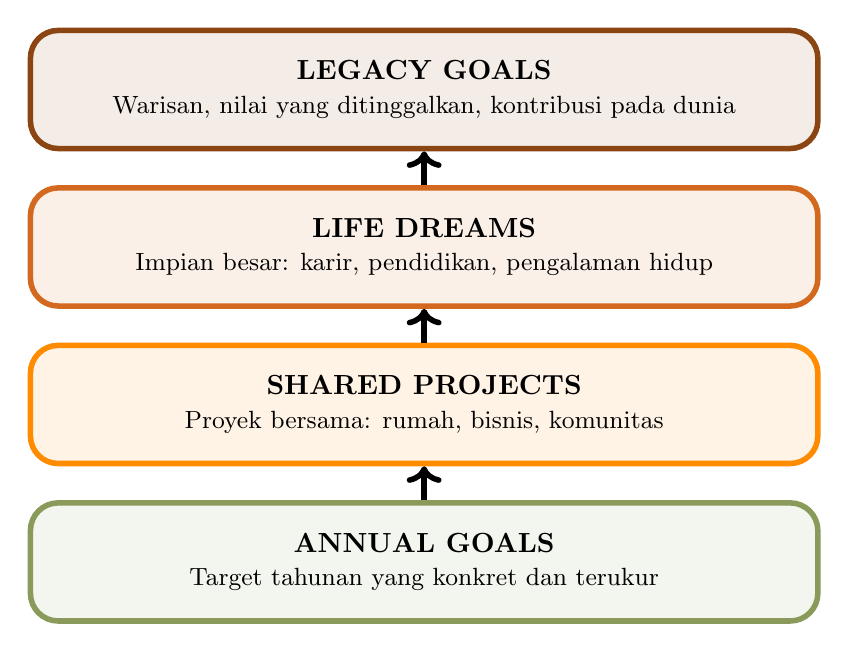
\begin{tikzpicture}[
    goal/.style={draw=#1, line width=2pt, rounded corners=10pt, fill=#1!10,
                 minimum width=10cm, minimum height=1.5cm, align=center}
]
    \node[goal=primary] (legacy) at (0,6) {
        \textbf{LEGACY GOALS}\\
        \small Warisan, nilai yang ditinggalkan, kontribusi pada dunia
    };
    
    \node[goal=secondary] (life) at (0,4) {
        \textbf{LIFE DREAMS}\\
        \small Impian besar: karir, pendidikan, pengalaman hidup
    };
    
    \node[goal=accent] (shared) at (0,2) {
        \textbf{SHARED PROJECTS}\\
        \small Proyek bersama: rumah, bisnis, komunitas
    };
    
    \node[goal=sagegreen] (annual) at (0,0) {
        \textbf{ANNUAL GOALS}\\
        \small Target tahunan yang konkret dan terukur
    };
    
    \draw[->, line width=2pt] (annual) -- (shared);
    \draw[->, line width=2pt] (shared) -- (life);
    \draw[->, line width=2pt] (life) -- (legacy);
\end{tikzpicture}
\end{center}

\subsection{Shared Goals Exercise}

\begin{exercisebox}[Worksheet: Goals Alignment]
\textbf{Petunjuk:} Jawab secara individual, lalu diskusikan dan cari overlap.

\subsection*{A. Personal Dreams (Individual)}
\begin{enumerate}
    \item Jika uang dan waktu tidak masalah, apa yang ingin kamu capai dalam 5 tahun?
    \item Apa legacy pribadi yang ingin kamu tinggalkan?
    \item Apa pengalaman hidup yang paling ingin kamu miliki?
\end{enumerate}

\subsection*{B. Shared Dreams (Bersama)}
\begin{enumerate}
    \item[4.] Apa yang ingin kita capai \textbf{bersama} dalam 1 tahun?
    \item[5.] Apa yang ingin kita capai \textbf{bersama} dalam 5 tahun?
    \item[6.] Apa yang ingin kita capai \textbf{bersama} dalam 20 tahun?
    \item[7.] Bagaimana kita ingin diingat oleh anak/cucu kita?
\end{enumerate}

\subsection*{C. Alignment Check}
Untuk setiap tujuan di atas, diskusikan:
\begin{itemize}
    \item Apakah tujuan pribadi kita saling mendukung atau bertentangan?
    \item Apa yang perlu dikorbankan untuk tujuan bersama?
    \item Bagaimana kita akan memantau progress?
\end{itemize}

\textbf{Action Items:}
\begin{enumerate}
    \item \rule{12cm}{0.4pt}
    \item \rule{12cm}{0.4pt}
    \item \rule{12cm}{0.4pt}
\end{enumerate}
\end{exercisebox}

\section{Level 4: Symbols---Makna di Balik Objek dan Konsep}

\keyterm{Symbols} adalah objek, tempat, atau konsep yang memiliki makna lebih dalam bagi hubungan. Ini adalah ``bahasa rahasia'' pasangan.

\subsection{Kategori Simbol}

\begin{center}
\renewcommand{\arraystretch}{1.6}
\begin{tabular}{|>{\raggedright}p{3cm}|>{\raggedright}p{4.5cm}|>{\raggedright}p{4.5cm}|>{\raggedright\arraybackslash}p{3cm}|}
\hline
\rowcolor{primary!20}
\textbf{Simbol} & \textbf{Makna Potensial} & \textbf{Diskusi yang Diperlukan} & \textbf{Contoh Konflik} \\
\hline
\textbf{Home} & Security, creativity, status, comfort & Apa fungsi utama rumah? Apa yang membuatnya ``berhasil''? & Minimalis vs collector \\
\hline
\textbf{Money} & Security, freedom, success, enjoyment & Mengapa kita menabak/belanja? Uang untuk apa? & Saver vs spender \\
\hline
\textbf{Time} & Productivity, presence, achievement, connection & Apa makna waktu yang ``well-spent''? & Workaholic vs quality time seeker \\
\hline
\textbf{Sex} & Intimacy, pleasure, obligation, power & Apa makna keintiman fisik? & High vs low desire \\
\hline
\textbf{Work} & Identity, provision, passion, burden & Apa peran kerja dalam hidup? & Ambisi vs balance \\
\hline
\textbf{Family} & Obligation, joy, burden, identity & Seberapa dekat dengan keluarga besar? & Enmeshed vs independent \\
\hline
\end{tabular}
\end{center}

\subsection{Menjelajahi Makna Simbol}

\begin{tipbox}[Dialog tentang Simbol]
\textbf{Home:}
\begin{itemize}
    \item ``Ceritakan tentang rumah masa kecilmu. Bagaimana rasanya?''
    \item ``Apa yang membuatmu merasa `pulang'?''
    \item ``Rumah ideal kita seperti apa? Kenapa?''
\end{itemize}

\textbf{Money:}
\begin{itemize}
    \item ``Apa pengalaman pertamamu dengan uang?''
    \item ``Apa yang membuatmu cemas tentang uang?''
    \item ``Uang mewakili apa bagimu: security, freedom, atau yang lain?''
\end{itemize}

\textbf{Time:}
\begin{itemize}
    \item ``Apa memori terbaikmu tentang waktu bersama keluarga?''
    \item ``Kapan terakhir kali kamu merasa `hidup'? Apa yang terjadi?''
    \item ``Bagaimana kamu ingin menghabiskan waktu kalau hanya punya setahun lagi?''
\end{itemize}
\end{tipbox}

\section{Case Studies: Membangun Shared Meaning dari Nol}

\subsection{Case Study 1: Alex dan Maya---Pasangan Baru}

\begin{praktikbox}[Background]
\textbf{Situation:} Alex dan Maya menikah 2 tahun. Keduanya fokus pada karir masing-masing. Hubungan mulai terasa hampa---seperti ``roommate yang berbagi tempat tidur.''

\textbf{Assessment:}
\begin{itemize}
    \item Rituals: Hampir tidak ada rutinitas bersama
    \item Roles: Belum jelas ekspektasi masing-masing
    \item Goals: Target pribadi yang terpisah
    \item Symbols: Belum membicarakan makna uang, waktu, rumah
\end{itemize}
\end{praktikbox}

\begin{praktikbox}[Intervensi Shared Meaning]
\textbf{Step 1: Ritual Building}
\begin{itemize}
    \item Dibuat: Morning coffee ritual (15 menit tanpa HP)
    \item Dibuat: Weekly ``dream date'' (diskusi tentang impian, bukan tugas)
    \item Dibuat: Monthly ``adventure day'' (mencoba aktivitas baru bersama)
\end{itemize}

\textbf{Step 2: Roles Clarification}
\begin{itemize}
    \item Diskusi panjang tentang makna ``menjadi pasangan''
    \item Kesepakatan: ``Kami adalah tim. Kemenangan satu adalah kemenangan keduanya.''
    \item Pembagian tanggung jawab rumah tangga yang jelas
\end{itemize}

\textbf{Step 3: Goals Alignment}
\begin{itemize}
    \item Ditemukan: Keduanya ingin punya bisnis bersama suatu hari nanti
    \item Dibuat: 5-year plan dengan milestone bersama
    \item Dibuat: Annual goal review tradition
\end{itemize}

\textbf{Step 4: Symbols Exploration}
\begin{itemize}
    \item Alex: Uang = freedom (dari kemiskinan masa kecil)
    \item Maya: Uang = security (orang tuanya bercerai karena utang)
    \item Agreement: 60\% needs, 20\% fun money masing-masing, 20\% dreams
\end{itemize}
\end{praktikbox}

\begin{praktikbox}[Result: After 6 Months]
\begin{itemize}
    \item Morning ritual menjadi ``sacred''---tidak pernah dilewatkan meski sibuk
    \item Monthly adventure date menjadi highlight yang dinantikan
    \item Shared business plan sedang dikerjakan---rasa tim terbentuk kuat
    \item Konflik uang berkurang karena saling memahami makna di baliknya
\end{itemize}
\end{praktikbox}

\subsection{Case Study 2: Budi dan Sari---Pasangan 15 Tahun}

\begin{praktikbox}[Background]
\textbf{Situation:} Budi dan Sari menikah 15 tahun, punya 2 anak remaja. Fokus sepenuhnya pada anak. Setelah anak mulai mandiri, mereka menyadari mereka ``tidak mengenal'' satu sama lain lagi.

\textbf{The Drift:}
\begin{itemize}
    \item Semua percakapan tentang anak atau logistik
    \item Tidak ada ritual berdua sejak anak lahir
    \item Peran: ``Ayah'' dan ``Ibu'' lebih kuat dari ``Suami'' dan ``Istri''
    \item Goals: Sepenuhnya terkait anak---tidak ada untuk mereka berdua
\end{itemize}
\end{praktikbox}

\begin{praktikbox}[Intervensi Shared Meaning]
\textbf{Step 1: Rekindling Rituals}
\begin{itemize}
    \item Dibuat: ``Second honeymoon''---trip berdua pertama dalam 10 tahun
    \item Dibuat: Weekly coffee date (seminggu sekali saat anak di sekolah)
    \item Dibuat: Nightly 10-minute check-in (sebelum tidur, tanpa anak)
\end{itemize}

\textbf{Step 2: Redefining Roles}
\begin{itemize}
    \item Diskusi: ``Siapa kita selain orang tua?''
    \item Discovery: Budi ingin kembali bermusik; Sari ingin menulis
    \item Agreement: Masing-masing punya waktu untuk passion pribadi
\end{itemize}

\textbf{Step 3: New Shared Goals}
\begin{itemize}
    \item Dibuat: ``Empty nest vision''---rencana untuk saat anak pergi
    \item Dibuat: Travel bucket list
    \item Dibuat: Joint hobby (memasak kursus)
\end{itemize}
\end{praktikbox}

\subsection{Case Study 3: David dan Rina---Visi Berbeda}

\begin{warningbox}[The Challenge]
\textbf{David:} Island type. Ingin pensiun dini, hidup sederhana di pegunungan, jauh dari keramaian.

\textbf{Rina:} Wave type. Ingin sukses besar, hidup di kota, aktif dalam komunitas sosial.

\textbf{Konflik:} Perbedaan visi hidup fundamental---bisa menjadi perpetual problem yang tidak terselesaikan.
\end{warningbox}

\begin{praktikbox}[Resolusi: Finding Shared Meaning dalam Perbedaan]
\textbf{Step 1: Dreams Within Conflict Dialogue}
\begin{itemize}
    \item David: Pegunungan = peace, recovery dari trauma kerja, kebebasan
    \item Rina: Kota = connection, purpose, validation, membuat perbedaan
\end{itemize}

\textbf{Step 2: Finding Common Ground}
\begin{itemize}
    \item Ditemukan: Keduanya ingin ``membuat perbedaan''---cara berbeda
    \item Ditemukan: Keduanya butuh ``ruang aman''---definisi berbeda
    \item Ditemukan: Keduanya menghargai ``kebebasan''---ekspresi berbeda
\end{itemize}

\textbf{Step 3: Creative Compromise}
\begin{itemize}
    \item Agreement: 6 bulan kota, 6 bulan pegunungan (setelah pensiun)
    \item Agreement: David akan volunteer di komunitas Rina
    \item Agreement: Rina akan bantu David membangun komunitas di pegunungan
    \item Agreement: Selama ini---liburan regular ke kedua tempat
\end{itemize}
\end{praktikbox}

\section{Ketika Pasangan Punya Visi Berbeda: Cara Negosiasi}

\begin{warningbox}[Realitas Perbedaan]
Tidak semua pasangan akan sepenuhnya setuju tentang shared meaning. Perbedaan dalam:
\begin{itemize}
    \item Nilai fundamental (religious, moral)
    \item Lifestyle preferences (city vs country, simple vs luxurious)
    \item Life goals (children vs childfree, career vs family focus)
    \item Attachment needs (Island vs Wave patterns)
\end{itemize}

\textit{Ini adalah \textbf{perpetual problems} yang perlu dikelola, bukan diselesaikan.}
\end{warningbox}

\subsection{Framework Negosiasi Shared Meaning}

\begin{center}
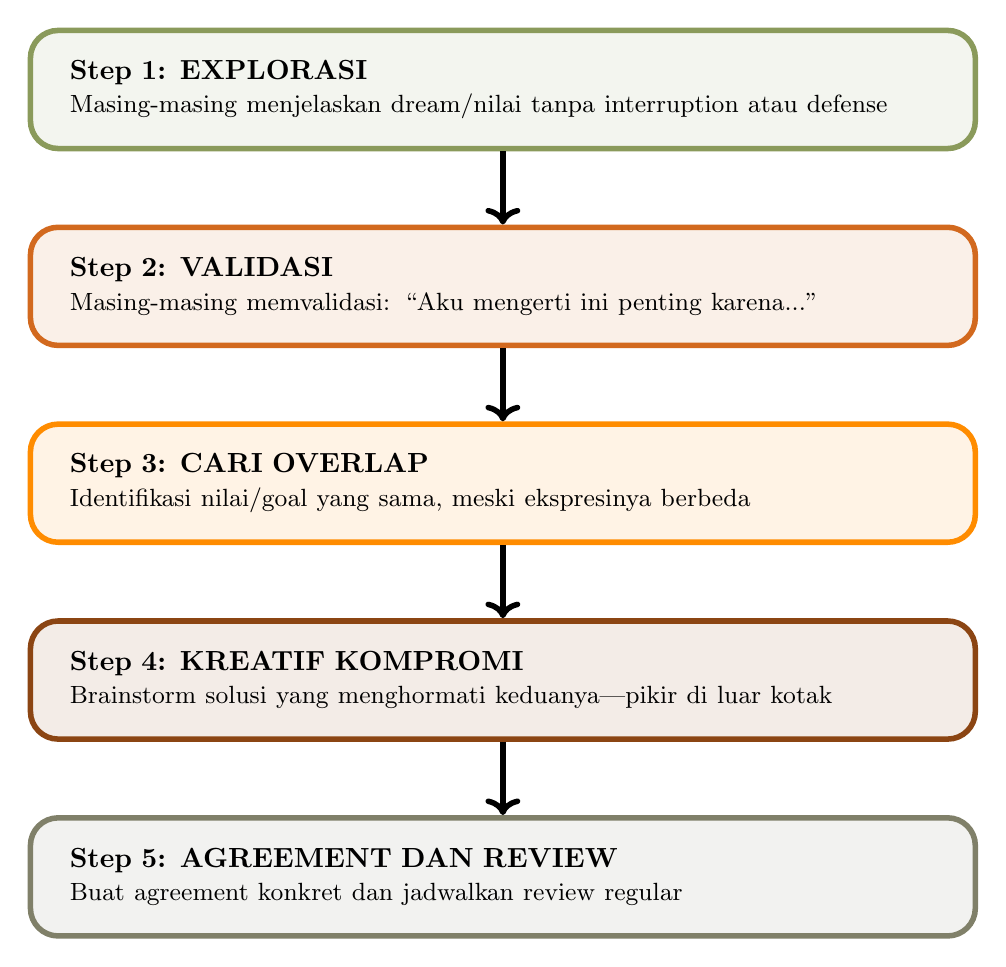
\begin{tikzpicture}[
    step/.style={draw=#1, line width=2pt, rounded corners=10pt, fill=#1!10,
                  minimum width=12cm, minimum height=1.5cm, align=left, text width=11cm}
]
    \node[step=sagegreen] (s1) at (0,8) {
        \textbf{Step 1: EXPLORASI}\\
        \small Masing-masing menjelaskan dream/nilai tanpa interruption atau defense
    };
    
    \node[step=secondary] (s2) at (0,5.5) {
        \textbf{Step 2: VALIDASI}\\
        \small Masing-masing memvalidasi: ``Aku mengerti ini penting karena...''
    };
    
    \node[step=accent] (s3) at (0,3) {
        \textbf{Step 3: CARI OVERLAP}\\
        \small Identifikasi nilai/goal yang sama, meski ekspresinya berbeda
    };
    
    \node[step=primary] (s4) at (0,0.5) {
        \textbf{Step 4: KREATIF KOMPROMI}\\
        \small Brainstorm solusi yang menghormati keduanya---pikir di luar kotak
    };
    
    \node[step=warmgray] (s5) at (0,-2) {
        \textbf{Step 5: AGREEMENT DAN REVIEW}\\
        \small Buat agreement konkret dan jadwalkan review regular
    };
    
    \draw[->, line width=2pt] (s1) -- (s2);
    \draw[->, line width=2pt] (s2) -- (s3);
    \draw[->, line width=2pt] (s3) -- (s4);
    \draw[->, line width=2pt] (s4) -- (s5);
\end{tikzpicture}
\end{center}

\subsection{Teknik Kompromi Kreatif}

\begin{tipbox}[Strategi Negosiasi]
\textbf{1. The Time-Division Solution}
\begin{itemize}
    \item ``6 bulan di A, 6 bulan di B''
    \item ``Weekdays untuk X, weekends untuk Y''
    \item ``Fase 1: X, Fase 2: Y''
\end{itemize}

\textbf{2. The Hybrid Solution}
\begin{itemize}
    \item Gabungkan elemen dari keduanya
    \item Contoh: Hidup di kota dengan balkon taman (city + nature)
\end{itemize}

\textbf{3. The Autonomy Agreement}
\begin{itemize}
    \item ``Kamu lakukan X, aku lakukan Y, kita respect pilihan masing-masing''
    \item Contoh: Satu fokus karir, satu fokus keluarga---tapi keduanya valid
\end{itemize}

\textbf{4. The Trial Period}
\begin{itemize}
    \item Coba satu cara selama periode tertentu, lalu evaluasi
    \item Coba cara lain, bandingkan
\end{itemize}

\textbf{5. The Third Way}
\begin{itemize}
    \item Brainstorm opsi C yang tidak dipikirkan sebelumnya
    \item Minta input dari counselor, mentor, atau teman bijak
\end{itemize}
\end{tipbox}

\section{Integrasi dengan Attachment Styles}

\begin{center}
\renewcommand{\arraystretch}{1.7}
\begin{tabular}{|>{\raggedright}p{2.5cm}|>{\raggedright}p{5cm}|>{\raggedright}p{5cm}|}
\hline
\rowcolor{primary!20}
\textbf{Attachment} & \textbf{Biasa dalam Shared Meaning} & \textbf{Strategi Optimal} \\
\hline
\textbf{Anchor} & Natural dalam membangun shared meaning; balance individual dan shared goals & Gunakan kekuatan untuk memfasilitasi diskusi; bantu pasangan yang struggle \\
\hline
\textbf{Island} & Cenderung fokus pada goals individual; sulit dengan ``interdependent'' rituals & Beri ruang autonomy dalam shared meaning; ritual jangan terlalu ``melekat'' \\
\hline
\textbf{Wave} & Kuat dalam emotional rituals; mungkin terlalu fokus pada togetherness & Balance dengan individual goals; pastikan tidak mengorbankan diri sendiri \\
\hline
\end{tabular}
\end{center}

\subsection{Challenges by Combination}

\begin{praktikbox}[Island + Wave dalam Shared Meaning]
\textbf{Challenge:}
\begin{itemize}
    \item Wave ingin banyak shared rituals (koneksi)
    \item Island ingin individual space (autonomy)
    \item Risiko: Wave merasa ditinggal, Island merasa tercekik
\end{itemize}

\textbf{Solution:}
\begin{itemize}
    \item Rituals yang ada ``escape clause''-nya
    \item Balance: Some together, some apart
    \item Agreement yang jelas tentang ``me time''
\end{itemize}
\end{praktikbox}

\begin{praktikbox}[Two Islands dalam Shared Meaning]
\textbf{Challenge:}
\begin{itemize}
    \item Keduanya fokus pada goals individual
    \item Risiko: Hubungan menjadi ``parallel lives''
    \item Sedikit emotional investment dalam ``bersama''
\end{itemize}

\textbf{Solution:}
\begin{itemize}
    \item Scheduled shared meaning activities (wajib)
    \item External accountability (counselor, friends)
    \item Practical shared goals (bisnis, proyek rumah)
\end{itemize}
\end{praktikbox}

\begin{praktikbox}[Two Waves dalam Shared Meaning]
\textbf{Challenge:}
\begin{itemize}
    \item Terlalu banyak fokus pada ``kita'', sedikit individual identity
    \item Risiko: Codependency, loss of self
    \item Emosi yang terlalu terkait satu sama lain
\end{itemize}

\textbf{Solution:}
\begin{itemize}
    \item Sengaja maintain individual friendships/hobbies
    \item Rituals yang support individual growth
    \item Regular check: ``Apa kebutuhanku sendiri?''
\end{itemize}
\end{praktikbox}

\section{Annual Relationship Review: Template}

\begin{exercisebox}[TEMPLATE: Annual Relationship Review]
\textbf{Tanggal:} \rule{4cm}{0.4pt} \textbf{Tempat:} \rule{5cm}{0.4pt}

\textit{(Blokir 3-4 jam. Bawa notes tahun lalu jika ada.)}

\subsection*{BAGIAN A: Year in Review (30 menit)}
\begin{enumerate}
    \item Apa pencapaian terbesar hubungan kita tahun ini?
    \item Apa tantangan terbesar yang kita hadapi?
    \item Apa momen paling berkesan bersama?
    \item Apa yang kita pelajari tentang satu sama lain?
    \item Apa yang kita pelajari tentang hubungan kita?
\end{enumerate}

\subsection*{BAGIAN B: Rituals Review (20 menit)}
\begin{enumerate}
    \item Ritual apa yang berjalan baik tahun ini?
    \item Ritual apa yang terbengkalai dan perlu di-revive?
    \item Ritual baru apa yang ingin kita coba tahun depan?
    \item Apa yang membuat ritual kita berharga?
\end{enumerate}

\subsection*{BAGIAN C: Roles Check-in (20 menit)}
\begin{enumerate}
    \item Apakah peran kita sebagai pasangan masih sesuai ekspektasi?
    \item Ada perubahan dalam peran (karir, parenting, dll)?
    \item Apa yang ingin kita ubah dalam cara kita menjalankan peran?
\end{enumerate}

\subsection*{BAGIAN D: Goals Progress (30 menit)}
\begin{enumerate}
    \item Review goals tahun lalu---apa yang tercapai?
    \item Apa yang belum tercapai dan mengapa?
    \item Goals baru untuk tahun depan:
    \begin{itemize}
        \item Individual: \rule{8cm}{0.4pt}
        \item Shared: \rule{8cm}{0.4pt}
    \end{itemize}
\end{enumerate}

\subsection*{BAGIAN E: Symbols Exploration (20 menit)}
\begin{enumerate}
    \item Apakah makna dari rumah, uang, waktu berubah tahun ini?
    \item Apa yang perlu kita klaim ulang atau redefinisikan?
\end{enumerate}

\subsection*{BAGIAN F: Looking Forward (20 menit)}
\begin{enumerate}
    \item Visi besar: Di mana kita ingin berada dalam 5 tahun?
    \item Prioritas #1 untuk tahun depan:
    \item Komitmen masing-masing:
    \begin{itemize}
        \item Partner A: \rule{8cm}{0.4pt}
        \item Partner B: \rule{8cm}{0.4pt}
    \end{itemize}
\end{enumerate}

\subsection*{BAGIAN G: Celebration and Closing (10 menit)}
\begin{enumerate}
    \item Apresiasi untuk pasangan:
    \item Janji untuk tahun depan:
    \item Ritual penutup (pelukan, ciuman, doa bersama, dll):
\end{enumerate}

\vspace{0.5cm}
\textbf{Ditandatangani:}\\
Partner A: \rule{5cm}{0.4pt} Tanggal: \rule{3cm}{0.4pt}\\
Partner B: \rule{5cm}{0.4pt} Tanggal: \rule{3cm}{0.4pt}

\vspace{0.5cm}
\textit{(Simpan ini. Review lagi tahun depan!)}
\end{exercisebox}

\section{Action Steps: Memulai Shared Meaning Journey}

\begin{exercisebox}[Program 30 Hari: Membangun Shared Meaning]

\textbf{MINGGU 1: Assessment dan Rituals}
\begin{itemize}
    \item \textbf{Hari 1-2:} Kerjakan Shared Meaning Assessment bersama
    \item \textbf{Hari 3-4:} Identifikasi ritual yang sudah ada (meski tidak disadari)
    \item \textbf{Hari 5-7:} Buat satu ritual baru dan mulai praktikkan
\end{itemize}

\textbf{MINGGU 2: Roles dan Goals}
\begin{itemize}
    \item \textbf{Hari 8-10:} Diskusikan makna peran masing-masing
    \item \textbf{Hari 11-14:} Kerjakan Goals Alignment worksheet
\end{itemize}

\textbf{MINGGU 3: Symbols dan Stories}
\begin{itemize}
    \item \textbf{Hari 15-17:} Dialog tentang simbol: rumah, uang, waktu
    \item \textbf{Hari 18-21:} Ceritakan ``story of us''---bagaimana hubungan ini berkembang
\end{itemize}

\textbf{MINGGU 4: Integration dan Commitment}
\begin{itemize}
    \item \textbf{Hari 22-25:} Buat Couple Agreement tentang shared meaning
    \item \textbf{Hari 26-28:} Jadwalkan Annual Review pertama
    \item \textbf{Hari 29-30:} Reflection dan celebration
\end{itemize}
\end{exercisebox}

\section{Kesimpulan: The Ultimate Goal}

\begin{insightbox}
\textbf{Key Takeaways Chapter 10:}

\begin{enumerate}
    \item \textbf{Shared meaning adalah puncak dari Seven Principles}---tempat di mana semua prinsip lain bermuara
    
    \item \textbf{Shared meaning melampaui daily logistics}---ini tentang makna hidup yang dibangun bersama
    
    \item \textbf{Empat pilar shared meaning:} Rituals, Roles, Goals, dan Symbols
    
    \item \textbf{Shared meaning bisa dibangun}---meski dimulai dari nol
    
    \item \textbf{Perbedaan dalam visi bukan akhir}---dengan dialog dan kreativitas, kompromi bermakna mungkin
    
    \item \textbf{Annual review menjaga shared meaning tetap hidup}---ini bukan ``set and forget''
\end{enumerate}

\textit{``Hubungan yang berhasil bukan hanya tentang bertahan dari badai. Ini tentang menciptakan peta bersama---menuju destinasi yang kalian bangun berdua.''} --- John Gottman
\end{insightbox}

\begin{tipbox}[Final Checklist]
\begin{itemize}
    \item[$\square$] Shared Meaning Assessment sudah dikerjakan
    \item[$\square$] Minimal satu ritual baru sudah dimulai
    \item[$\square$] Dialog tentang roles sudah dilakukan
    \item[$\square$] Goals alignment sudah dibahas
    \item[$\square$] Makna simbol kunci sudah dieksplorasi
    \item[$\square$] Annual Review sudah dijadwalkan
    \item[$\square$] Couple Agreement tentang shared meaning sudah dibuat
\end{itemize}
\end{tipbox}

\vspace{1cm}
\begin{center}

\begin{tikzpicture}
    \node[draw=primary, line width=3pt, rounded corners=20pt, 
          fill=lightbg, inner sep=30pt, align=center] {
        {\Large\bfseries\color{primary} Selamat!}\\[0.5cm]
        {\large\color{darktext} Kamu telah menyelesaikan semua}\\
        {\large\color{darktext} Seven Principles for Making Marriage Work.}\\[0.5cm]
        {\color{warmgray} Ingat: Ini bukan akhir, tapi awal.}\\
        {\color{warmgray} Shared meaning adalah perjalanan seumur hidup.}
    };
\end{tikzpicture}
\end{center}

\chapter{Couple Bubble: Gelembung Pasangan yang Melindungi}

\begin{insightbox}
\textit{``Couple Bubble bukanlah tentang isolasi dari dunia, melainkan tentang menciptakan zona aman di mana kalian berdua bisa saling melindungi. Ini adalah pakta mutual protection: \highlight{aku menjagamu, kamu menjagaku, dan kita menjaga \textit{kita} bersama}.''} --- Dr. Stan Tatkin
\end{insightbox}

\section{Memahami Konsep Couple Bubble}

\subsection{Apa itu Couple Bubble?}

\keyterm{Couple Bubble} adalah sebuah konsep yang dikembangkan oleh Dr. Stan Tatkin untuk menggambarkan \highlight{ruang psikologis dan emosional yang diciptakan oleh pasangan} untuk saling melindungi. Bayangkan sebuah gelembung transparan yang membungkus kalian berdua --- di dalamnya, kalian merasa aman, diterima, dan saling mendukung.

\begin{praktikbox}[Definisi Couple Bubble]
Couple Bubble adalah \textbf{kesepakatan implisit dan eksplisit} antara dua orang untuk:
\begin{itemize}
    \item Menempatkan keamanan hubungan sebagai prioritas utama
    \item Menjadi tempat perlindungan satu sama lain dari ancaman dunia luar
    \item Berkomitmen untuk saling menjaga, meski dalam konflik
    \item Membangun sistem kekebalan bersama terhadap tekanan eksternal
\end{itemize}
\end{praktikbox}

\subsection{Mengapa Couple Bubble Penting?}

Secara evolusioner, manusia adalah makhluk \textit{pair-bonding} --- kita butuh ikatan dengan pasangan untuk bertahan hidup dan berkembang biak. Otak kita \textit{wired} (terkabel) untuk:

\begin{enumerate}
    \item \textbf{Mencari keamanan} dalam hubungan dekat
    \item \textbf{Menggunakan pasangan} sebagai ``secure base'' untuk menjelajahi dunia
    \item \textbf{Saling menenangkan} saat stres (co-regulation)
\end{enumerate}

\begin{center}
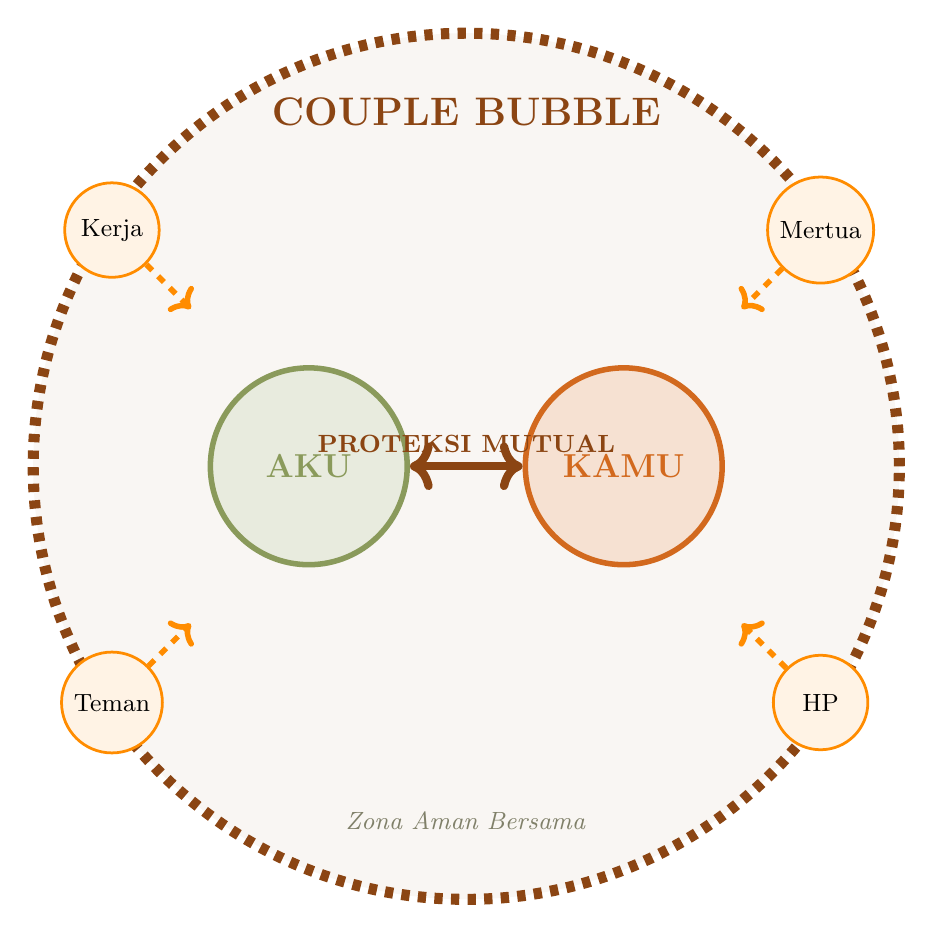
\begin{tikzpicture}[
    bubble/.style={draw=primary, line width=3pt, rounded corners=20pt, 
                   fill=lightbg, minimum width=12cm, minimum height=7cm, align=center}
]
    % Outer circle representing the bubble
    \draw[primary, line width=4pt, dashed, fill=primary!5] (0,0) circle (5.5cm);
    
    % Couple inside
    \node[circle, draw=sagegreen, line width=2pt, fill=sagegreen!20, minimum size=2.5cm] (p1) at (-2,0) {};
    \node[font=\large\bfseries, sagegreen] at (p1) {AKU};
    
    \node[circle, draw=secondary, line width=2pt, fill=secondary!20, minimum size=2.5cm] (p2) at (2,0) {};
    \node[font=\large\bfseries, secondary] at (p2) {KAMU};
    
    % Connection
    \draw[<->, line width=3pt, primary] (p1) -- (p2) node[midway, above, font=\small\bfseries] {PROTEKSI MUTUAL};
    
    % External threats
    \node[circle, draw=accent, line width=1pt, fill=accent!10, minimum size=1.2cm] (t1) at (-4.5,3) {\small Kerja};
    \node[circle, draw=accent, line width=1pt, fill=accent!10, minimum size=1.2cm] (t2) at (4.5,3) {\small Mertua};
    \node[circle, draw=accent, line width=1pt, fill=accent!10, minimum size=1.2cm] (t3) at (-4.5,-3) {\small Teman};
    \node[circle, draw=accent, line width=1pt, fill=accent!10, minimum size=1.2cm] (t4) at (4.5,-3) {\small HP};
    
    % Arrows showing protection
    \draw[->, line width=2pt, accent, dashed] (t1) -- (-3.5,2);
    \draw[->, line width=2pt, accent, dashed] (t2) -- (3.5,2);
    \draw[->, line width=2pt, accent, dashed] (t3) -- (-3.5,-2);
    \draw[->, line width=2pt, accent, dashed] (t4) -- (3.5,-2);
    
    % Bubble label
    \node[font=\Large\bfseries, primary] at (0,4.5) {COUPLE BUBBLE};
    \node[font=\small, warmgray] at (0,-4.5) {\textit{Zona Aman Bersama}};
\end{tikzpicture}
\end{center}

\subsection{Perbedaan Couple Bubble dan Ketergantungan Tidak Sehat}

\begin{warningbox}[Couple Bubble $\neq$ Codependency]
\textbf{Couple Bubble (Sehat):}
\begin{itemize}
    \item Dua individu utuh yang memilih untuk saling melindungi
    \item Batasan dengan dunia luar jelas tapi fleksibel
    \item Kedua pihak tetap bisa berfungsi secara independen
    \item Proteksi bersifat saling, bukan satu arah
\end{itemize}

\textbf{Codependency (Tidak Sehat):}
\begin{itemize}
    \item Satu pihak ``menyelamatkan'' pihak lain secara terus-menerus
    \item Batasan kabur atau tidak ada
    \item Kehilangan identitas individual
    \item Dinamasa yang tidak setara (caregiver-pasien)
\end{itemize}
\end{warningbox}

\section{Tiga Prinsip Fundamental Couple Bubble}

\subsection{Prinsip 1: Menempatkan Hubungan di Atas Segalanya}

Ini adalah pilar paling fundamental. Artinya: \highlight{kepentingan hubungan kalian berdua lebih penting daripada kebutuhan individu, pekerjaan, keluarga besar, atau teman}.

\begin{tipbox}[Contoh Prinsip 1 dalam Praktik]
\textbf{Situasi:} Pasanganmu memiliki hari yang buruk dan butuh bicara, tapi kamu sedang sibuk dengan deadline kerja.

\textbf{Tanpa Couple Bubble:} ``Aku sibuk, kita bicara nanti saja. Kerjaanku lebih penting.''

\textbf{Dengan Couple Bubble:} ``Aku melihat kamu butuhku sekarang. Beri aku 10 menit untuk menyelesaikan ini, lalu aku akan matikan laptop dan kita bicara. Hubungan kita lebih penting daripada deadline ini.''
\end{tipbox}

\subsection{Prinsip 2: Menjadi \textit{Go-To Person} Satu Sama Lain}

\keyterm{Go-to person} adalah orang pertama yang kamu hubungi saat:
\begin{itemize}
    \item Ada kabar baik (\textit{capitalization})
    \item Ada masalah atau stres
    \item Butuh pendapat atau saran
    \item Merasa takut, sedih, atau bingung
\end{itemize}

\begin{praktikbox}[Mengapa Go-To Person Penting?]
Otak kita membutuhkan \textbf{secure base} --- tempat yang aman untuk ``pulang'' secara emosional. Ketika pasanganmu menjadi go-to person-mu:
\begin{enumerate}
    \item Sistem sarafmu menjadi lebih rileks
    \item Kamu merasa diterima sepenuhnya
    \item Kepercayaan diri meningkat karena ada ``safety net''
    \item Resiliensi terhadap stres eksternal meningkat
\end{enumerate}

\textit{Couple yang kuat adalah couple di mana masing-masing berkata: ``Aku tidak perlu orang lain, aku punya dia/dia.''}
\end{praktikbox}

\subsection{Prinsip 3: Melindungi Satu Sama Lain dari Ancaman}

Ancaman bisa datang dari dua arah:

\begin{center}
\renewcommand{\arraystretch}{1.6}
\begin{tabular}{|>{\raggedright}p{3cm}|>{\raggedright}p{5.5cm}|>{\raggedright\arraybackslash}p{5.5cm}|}
\hline
\rowcolor{primary!20}
\textbf{Jenis Ancaman} & \textbf{Contoh} & \textbf{Cara Melindungi} \\
\hline
\textbf{Eksternal} & Tekanan kerja, kritik mertua, gosip teman, distraksi teknologi & Bersatu menghadapi, membuat batasan, saling menenangkan \\
\hline
\textbf{Internal} & Kebiasaan buruk sendiri, insecure attachment, trauma masa lalu & Mengingatkan dengan lembut, memberi reassurance, tidak menyalahkan \\
\hline
\textbf{Interpersonal} & Konflik antar pasangan, misunderstanding, resentmen & Repair cepat, jangan biarkan mengendap, prioritaskan hubungan \\
\hline
\end{tabular}
\end{center}

\section{Self-Assessment: Seberapa Kuat Couple Bubble-mu?}

\begin{exercisebox}[Kuesioner Kekuatan Couple Bubble]
\textbf{Petunjuk:} Jawablah dengan jujur menggunakan skala berikut:
\begin{center}
\textbf{1} = Sangat tidak setuju \quad | \quad \textbf{2} = Tidak setuju \quad | \quad \textbf{3} = Netral \quad | \quad \textbf{4} = Setuju \quad | \quad \textbf{5} = Sangat setuju
\end{center}

\subsection*{Dimensi 1: Prioritas Hubungan}

\begin{enumerate}
    \item Saat ada konflik antara kebutuhanku dan kebutuhan hubungan, aku biasanya memprioritaskan hubungan.
    \item Aku sering mengorbankan waktu pribadi demi menghabiskan waktu bersama pasangan.
    \item Saat pasangan butuhku, aku bisa meletakkan pekerjaan atau hobi sejenak.
    \item Aku merasa hubungan kami adalah aset paling berharga dalam hidupku.
\end{enumerate}

\subsection*{Dimensi 2: Saling Melindungi}

\begin{enumerate}
    \setcounter{enumi}{4}
    \item Aku merasa aman membagikan kelemahanku pada pasangan tanpa takut dihakimi.
    \item Pasangan sering membelaku saat aku dikritik orang lain.
    \item Kami berdua saling mendukung saat salah satu stres dengan hal luar.
    \item Aku percaya pasangan akan selalu ``ada untukku'' saat aku benar-benar butuh.
\end{enumerate}

\subsection*{Dimensi 3: Batasan dengan Dunia Luar}

\begin{enumerate}
    \setcounter{enumi}{8}
    \item Kami punya aturan bersama tentang penggunaan ponsel saat bersama.
    \item Kami bisa menolak permintaan keluarga/teman yang mengganggu waktu berdua.
    \item Aku tidak membicarakan masalah hubungan dengan orang lain tanpa persetujuan pasangan.
    \item Kami menjaga privasi hubungan dari interferensi orang luar.
\end{enumerate}

\subsection*{Dimensi 4: Resiliensi dalam Konflik}

\begin{enumerate}
    \setcounter{enumi}{12}
    \item Saat bertengkar, kami tetap merasa ``kita dalam tim yang sama.''
    \item Kami cepat melakukan repair setelah konflik.
    \item Bahkan saat marah, aku tidak mengancam akan pergi atau mengakhiri hubungan.
    \item Aku merasa kami bisa melewati apa pun asal bersama-sama.
\end{enumerate}

\subsection*{Skoring dan Interpretasi}

\begin{center}
\renewcommand{\arraystretch}{1.4}
\begin{tabular}{|c|c|l|}
\hline
\rowcolor{sagegreen!20}
\textbf{Total Skor} & \textbf{Kategori} & \textbf{Interpretasi} \\
\hline
56--70 & \textbf{Sangat Kuat} & Couple Bubble kalian sangat solid. Pertahankan dengan ritual harian. \\
\hline
42--55 & \textbf{Kuat} & Ada fondasi yang baik. Beberapa area bisa ditingkatkan. \\
\hline
28--41 & \textbf{Perlu Perhatian} & Bubble mulak berlubang. Segera lakukan perbaikan bersama. \\
\hline
14--27 & \textbf{Lemah} & Bubble dalam bahaya. Intervensi intensif diperlukan. \\
\hline
\end{tabular}
\end{center}
\end{exercisebox}

\section{Ancaman terhadap Couple Bubble}

\subsection{Ancaman Eksternal}

\begin{warningbox}[Musuh dari Luar]
\begin{enumerate}
    \item \textbf{Pekerjaan yang Menyerbu}
    \begin{itemize}
        \item Email dan chat kerja yang di-check terus-menerus
        \item Membawa pulang stres dan frustrasi kantor
        \item Mengutamakan deadline daripada pasangan
    \end{itemize}
    
    \item \textbf{Keluarga Besar (Mertua)}
    \begin{itemize}
        \item Interferensi dalam keputusan pasangan
        \item Kritik terhadap pasanganmu
        \item Menempatkan loyalty keluarga di atas pasangan
    \end{itemize}
    
    \item \textbf{Teman dan Sosial Media}
    \begin{itemize}
        \item Menghabiskan lebih banyak waktu dengan teman daripada pasangan
        \item Membagi masalah hubungan di media sosial
        \item Teman yang meremehkan pasanganmu
    \end{itemize}
    
    \item \textbf{Smartphone dan Digital Distraction}
    \begin{itemize}
        \item Phubbing (phone + snubbing) --- mengabaikan pasangan karena ponsel
        \item Mengobrol dengan orang lain saat waktu bersama pasangan
        \item Tidak ada ``sacred space'' bebas gadget
    \end{itemize}
\end{enumerate}
\end{warningbox}

\subsection{Ancaman Internal}

\begin{center}
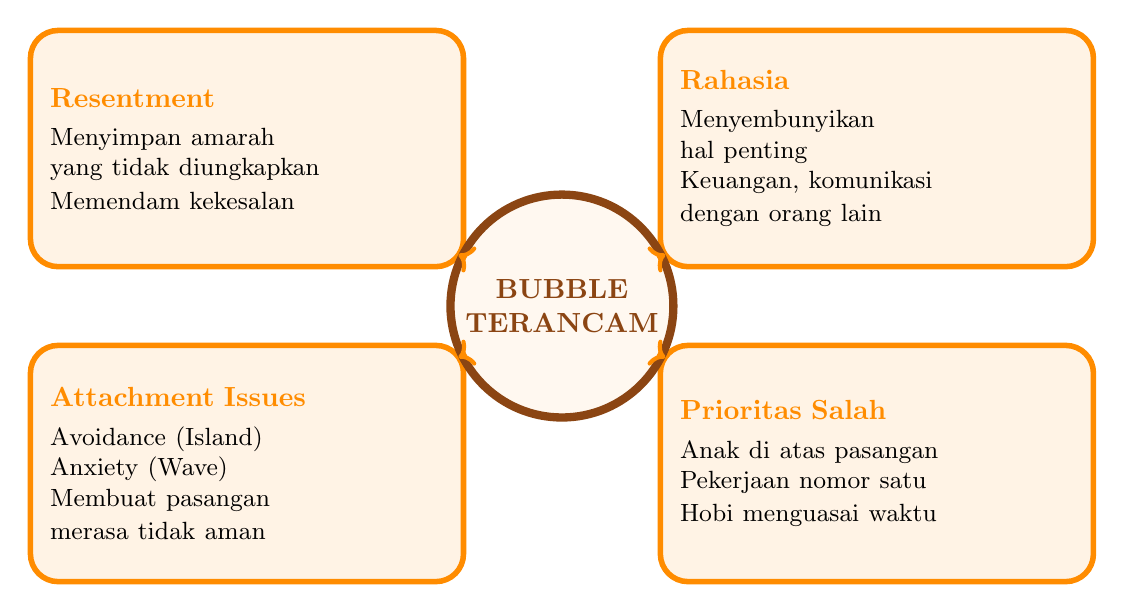
\begin{tikzpicture}[
    threat/.style={draw=#1, line width=2pt, rounded corners=10pt,
                   fill=#1!10, minimum width=5.5cm, minimum height=3cm, align=left, text width=5cm}
]
    % Internal threats
    \node[threat=accent] (i1) at (-4,2) {
        \textbf{\textcolor{accent}{Resentment}}\\[0.1cm]
        \small Menyimpan amarah\\
        \small yang tidak diungkapkan\\
        \small Memendam kekesalan
    };
    
    \node[threat=accent] (i2) at (4,2) {
        \textbf{\textcolor{accent}{Rahasia}}\\[0.1cm]
        \small Menyembunyikan\\
        \small hal penting\\
        \small Keuangan, komunikasi\\
        \small dengan orang lain
    };
    
    \node[threat=accent] (i3) at (-4,-2) {
        \textbf{\textcolor{accent}{Attachment Issues}}\\[0.1cm]
        \small Avoidance (Island)\\
        \small Anxiety (Wave)\\
        \small Membuat pasangan\\
        \small merasa tidak aman
    };
    
    \node[threat=accent] (i4) at (4,-2) {
        \textbf{\textcolor{accent}{Prioritas Salah}}\\[0.1cm]
        \small Anak di atas pasangan\\
        \small Pekerjaan nomor satu\\
        \small Hobi menguasai waktu
    };
    
    % Center bubble
    \node[circle, draw=primary, line width=3pt, fill=lightbg, minimum size=2.5cm, align=center, font=\bfseries\color{primary}] (center) at (0,0) {BUBBLE\\TERANCAM};
    
    % Arrows
    \draw[->, line width=1.5pt, accent] (i1) -- (center);
    \draw[->, line width=1.5pt, accent] (i2) -- (center);
    \draw[->, line width=1.5pt, accent] (i3) -- (center);
    \draw[->, line width=1.5pt, accent] (i4) -- (center);
\end{tikzpicture}
\end{center}

\begin{praktikbox}[Mengenali Tanda-Tanda Bubble Bermasalah]
\textbf{Sinyal Awal (Kuning):}
\begin{itemize}
    \item JarangQuality time tanpa gangguan
    \item Mengobrol dengan orang lain tentang pasangan (komplain)
    \item Merasa lebih nyaman sendiri atau dengan teman
\end{itemize}

\textbf{Sinyal Bahaya (Merah):}
\begin{itemize}
    \item Berpikir ``Aku lebih bahagia tanpa dia/dia''
    \item Menyimpan rahasia besar dari pasangan
    \item Fantasi tentang orang lain atau hidup tanpa pasangan
    \item Tidak merasa ``tim'' saat menghadapi masalah
\end{itemize}
\end{praktikbox}

\section{Membangun Couple Bubble: Panduan Langkah demi Langkah}

\subsection{Langkah 1: Komitmen Bersama}

Buat kesepakatan formal bersama. Tuliskan dan tanda tangani.

\begin{exercisebox}[Template Komitmen Couple Bubble]
\textbf{KOMITMEN COUPLE BUBBLE}

Kami, \underline{\hspace{4cm}} dan \underline{\hspace{4cm}}, 
sepakat untuk membangun dan menjaga Couple Bubble kami dengan komitmen sebagai berikut:

\textbf{1. PRIORITAS HUBUNGAN}
\begin{itemize}
    \item[$\square$] Hubungan kami adalah prioritas utama setelah kesehatan dan keselamatan
    \item[$\square$] Kami akan selalu memikirkan ``apa yang terbaik untuk kita'' sebelum mengambil keputusan besar
    \item[$\square$] Kami berkomitmen untuk menghabiskan waktu berkualitas minimal \underline{\hspace{2cm}} per minggu
\end{itemize}

\textbf{2. PROTEKSI MUTUAL}
\begin{itemize}
    \item[$\square$] Aku akan selalu ada untukmu saat kamu butuh, meski aku sedang sibuk
    \item[$\square$] Kami akan saling melindungi dari interferensi eksternal (kerja, keluarga, teman)
    \item[$\square$] Kami tidak akan membicarakan masalah kami dengan orang luar tanpa persetujuan bersama
\end{itemize}

\textbf{3. KOMUNIKASI}
\begin{itemize}
    \item[$\square$] Kami akan berbicara dengan jujur tentang kebutuhan dan kekhawatiran
    \item[$\square$] Kami akan melakukan repair secepatnya setelah konflik
    \item[$\square$] Kami akan menggunakan ``stress-reducing conversation'' minimal 20 menit per hari
\end{itemize}

\textbf{4. BATASAN}
\begin{itemize}
    \item[$\square$] Kami akan punya ``no-phone zone'' dan ``no-phone time'' bersama
    \item[$\square$] Kami bisa menolak permintaan yang mengganggu waktu berdua
    \item[$\square$] Privasi hubungan kami dijaga dari media sosial
\end{itemize}

\vspace{0.5cm}
Tanda tangan:\\[0.3cm]
\underline{\hspace{6cm}} \quad Tanggal: \underline{\hspace{3cm}}\\[0.2cm]
(\textit{Pasangan 1})\\[0.5cm]
\underline{\hspace{6cm}} \quad Tanggal: \underline{\hspace{3cm}}\\[0.2cm]
(\textit{Pasangan 2})
\end{exercisebox}

\subsection{Langkah 2: Membangun Ritual Koneksi}

\begin{tipbox}[Ritual Harian untuk Bubble Kuat]
\textbf{Pagi (5-10 menit):}
\begin{itemize}
    \item Sapaan hangat dengan kontak mata dan pelukan
    \item Tanya: ``Ada yang perlu kuketahui untuk hari ini?''
    \item Janji akan kembali dengan selamat
\end{itemize}

\textbf{Siang (1-2 menit):}
\begin{itemize}
    \item Pesan singkat: ``Thinking of you'' atau ``Semangat!''
    \item Tidak untuk diskusi panjang, hanya penanda ``aku di sini''
\end{itemize}

\textbf{Malam (20+ menit):}
\begin{itemize}
    \item Stress-reducing conversation (dengarkan tanpa solusi)
    \item Physical affection: pegang tangan, peluk, ciuman
    \item Ritual tidur: bersamaan, sentuhan sebelum tidur
\end{itemize}
\end{tipbox}

\subsection{Langkah 3: Membuat Batasan yang Jelas}

\begin{center}
\renewcommand{\arraystretch}{1.5}
\begin{tabular}{|>{\raggedright}p{4cm}|>{\raggedright}p{5cm}|>{\raggedright\arraybackslash}p{5cm}|}
\hline
\rowcolor{sagegreen!20}
\textbf{Area} & \textbf{Batasan yang Sehat} & \textbf{Implementasi} \\
\hline
Penggunaan ponsel & Tidak ponsel saat makan dan 1 jam sebelum tidur & Taruh di tempat tertentu, gunakan mode DND \\
\hline
Waktu kerja & Kerja tetap di kantor/ruang kerja, tidak ``bawa pulang'' & Buat ritual transisi: mandi, ganti baju sebelum quality time \\
\hline
Keluarga besar & Keputusan penting dibahas berdua dulu & Komunikasikan pada keluarga: ``Kami akan diskusi dulu'' \\
\hline
Teman & Waktu dengan teman tidak menggantikan date night & Jadwalkan teman di luar waktu prioritas pasangan \\
\hline
Media sosial & Tidak posting masalah hubungan & Agreement: tanya izin sebelum posting foto pasangan \\
\hline
\end{tabular}
\end{center}

\section{Maintenance Harian untuk Couple Bubble}

\begin{praktikbox}[Checklist Pemeliharaan Bubble]
\textbf{Setiap Hari (minimal):}
\begin{itemize}
    \item[$\square$] Morning greeting dengan kontak fisik (minimal 6 detik pelukan)
    \item[$\square$] 20 menit stress-reducing conversation
    \item[$\square$] Satu momen appreciation: ``Aku suka karena kamu...''
    \item[$\square$] Physical touch sebelum tidur
    \item[$\square$] Check-in singkat via pesan saat terpisah
\end{itemize}

\textbf{Setiap Minggu:}
\begin{itemize}
    \item[$\square$] Date night 2+ jam tanpa gangguan (no phone!)
    \item[$\square$] State of the Union meeting: ``Gimana hubungan kita minggu ini?''
    \item[$\square$] Satu aktivitas bersama yang menyenangkan
    \item[$\square$] Review: Apa yang berhasil? Apa yang perlu diperbaiki?
\end{itemize}

\textbf{Setiap Bulan:}
\begin{itemize}
    \item[$\square$] Review dan update Couple Agreement
    \item[$\square$] Planning untuk bulan depan (date, goals)
    \item[$\square$] Revisit Love Maps (update pengetahuan tentang pasangan)
\end{itemize}
\end{praktikbox}

\section{Perbaikan Darurat Saat Bubble Bocor}

\begin{warningbox}[Tanda Bubble dalam Bahaya]
\begin{enumerate}
    \item Salah satu pihak mengatakan ``Aku sudah tidak yakin dengan kita''
    \item Terjadi pengkhianatan kepercayaan (kebohongan besar, selingkuh emosional/fisik)
    \item Resentmen yang mendalam dan mengendap
    \item Kehilangan ikatan intem (tidak merasa ``kita'' lagi)
    \item Ancaman perceraian/pengakhiran hubungan sering muncul
\end{enumerate}
\end{warningbox}

\subsection{Protokol Perbaikan Darurat}

\begin{center}
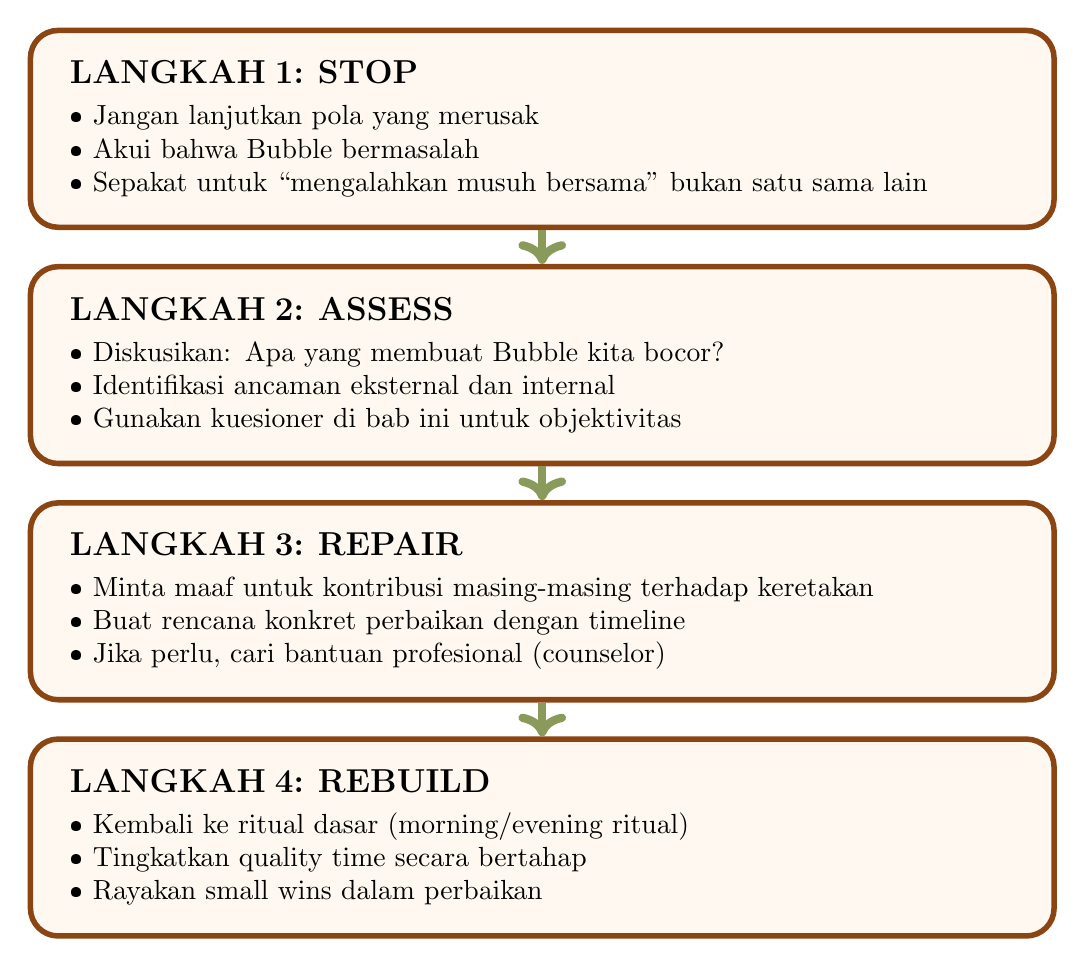
\begin{tikzpicture}[
    stepbox/.style={draw=primary, line width=2pt, rounded corners=10pt,
                 fill=lightbg, minimum width=13cm, minimum height=2.5cm, align=left, text width=12cm}
]
    \node[stepbox] (s1) at (0,6) {
        \textbf{\large LANGKAH 1: STOP}\\[0.1cm]
        \textbullet\ Jangan lanjutkan pola yang merusak\\
        \textbullet\ Akui bahwa Bubble bermasalah\\
        \textbullet\ Sepakat untuk ``mengalahkan musuh bersama'' bukan satu sama lain
    };
    
    \node[stepbox] (s2) at (0,3) {
        \textbf{\large LANGKAH 2: ASSESS}\\[0.1cm]
        \textbullet\ Diskusikan: Apa yang membuat Bubble kita bocor?\\
        \textbullet\ Identifikasi ancaman eksternal dan internal\\
        \textbullet\ Gunakan kuesioner di bab ini untuk objektivitas
    };
    
    \node[stepbox] (s3) at (0,0) {
        \textbf{\large LANGKAH 3: REPAIR}\\[0.1cm]
        \textbullet\ Minta maaf untuk kontribusi masing-masing terhadap keretakan\\
        \textbullet\ Buat rencana konkret perbaikan dengan timeline\\
        \textbullet\ Jika perlu, cari bantuan profesional (counselor)
    };
    
    \node[stepbox] (s4) at (0,-3) {
        \textbf{\large LANGKAH 4: REBUILD}\\[0.1cm]
        \textbullet\ Kembali ke ritual dasar (morning/evening ritual)\\
        \textbullet\ Tingkatkan quality time secara bertahap\\
        \textbullet\ Rayakan small wins dalam perbaikan
    };
    
    % Arrows
    \draw[->, line width=3pt, sagegreen] (s1) -- (s2);
    \draw[->, line width=3pt, sagegreen] (s2) -- (s3);
    \draw[->, line width=3pt, sagegreen] (s3) -- (s4);
\end{tikzpicture}
\end{center}

\begin{tipbox}[Teknik Repair Cepat]
\textbf{Jika baru terjadi konflik atau kesalahpahaman:}

\begin{enumerate}
    \item \textbf{The Pause} --- Beri jeda 20-30 menit agar sistem saraf tenang
    \item \textbf{The Approach} --- Salah satu mendekati dengan sikap terbuka
    \item \textbf{The Validation} --- ``Aku mengerti kamu merasa...'' (tanpa pembelaan)
    \item \textbf{The Ownership} --- ``Maaf aku sudah...'' (akui bagianmu)
    \item \textbf{The Reconnect} --- Sentuhan fisik (pegang tangan/peluk) untuk mengaktifkan oxytocin
    \item \textbf{The Plan} --- Diskusikan apa yang bisa dilakukan berbeda
\end{enumerate}

\textit{Ingat: Tujuan bukan memenangkan argumen, tapi memenangkan hubungan.}
\end{tipbox}

\section{Integrasi dengan Gaya Koneksi (Attachment Styles)}

Setiap tipe attachment membutuhkan pendekatan berbeda dalam membangun Bubble:

\subsection{Anchor (Secure) Membangun Bubble}

\begin{praktikbox}[Kekuatan Anchor dalam Couple Bubble]
\textbf{Yang Natural:}
\begin{itemize}
    \item Mudah membuat pasangan merasa prioritas
    \item Balance antara dekat dan memberi ruang
    \item Komunikasi terbuka tentang kebutuhan
\end{itemize}

\textbf{Yang Perlu Diperhatikan:}
\begin{itemize}
    \item Jangan jadi ``rescuer'' yang selalu mengorbankan diri
    \item Pastikan pasangan insecure juga berinvestasi
    \item Tetap jaga ritual meski merasa ``aman''
\end{itemize}
\end{praktikbox}

\subsection{Island (Avoidant) Membangun Bubble}

\begin{warningbox}[Tantangan Island]
\textbf{Hambatan internal Island:}
\begin{itemize}
    \item ``Couple Bubble terasa seperti jebakan/kurungan''
    \item ``Aku butuh ruang, jangan terlalu dekat''
    \item Sulit meminta bantuan atau menunjukkan kebutuhan
    \item Tendensi untuk mengutamakan pekerjaan/hobi di atas hubungan
\end{itemize}

\textbf{Strategi untuk Island:}
\begin{enumerate}
    \item \textbf{Reframe Bubble:} Ini bukan kurungan, ini basis operasi untuk menjelajahi dunia
    \item \textbf{Schedule alone time:} Negosiasi waktu sendiri yang jelas dalam Bubble
    \item \textbf{Gradual intimacy:} Perlahan-lahan buka diri, jangan dipaksa
    \item \textbf{Explicit commitment:} Ucapkan komitmen verbal meski terasa canggung
\end{enumerate}
\end{warningbox}

\subsection{Wave (Anxious) Membangun Bubble}

\begin{warningbox}[Tantangan Wave]
\textbf{Hambatan internal Wave:}
\begin{itemize}
    \item Takut Bubble akan pecah kapan saja
    \item Tendensi ``test'' dengan menciptakan konflik
    \item Klaim terlalu banyak waktu pasangan
    \item Sulit percaya pada komitmen pasangan
\end{itemize}

\textbf{Strategi untuk Wave:}
\begin{enumerate}
    \item \textbf{Self-soothing:} Latih menenangkan diri sebelum ``membanjiri'' pasangan
    \item \textbf{Trust the process:} Beri waktu untuk bukti komitmen
    \item \textbf{Communicate needs clearly:} Minta reassurance langsung, tidak lewat test
    \item \textbf{Celebrate security:} Apresiasi saat Bubble terasa kuat
\end{enumerate}
\end{warningbox}

\begin{center}
\renewcommand{\arraystretch}{1.6}
\begin{tabular}{|>{\raggedright}p{2.5cm}|>{\raggedright}p{4cm}|>{\raggedright}p{4cm}|>{\raggedright\arraybackslash}p{4cm}|}
\hline
\rowcolor{primary!20}
\textbf{Tipe} & \textbf{Kontribusi ke Bubble} & \textbf{Yang Perlu Dikerjakan} & \textbf{Partner Support} \\
\hline
\textbf{Anchor} & Stabilitas, kemudahan intimacy, komunikasi jelas & Jangan mengabaikan maintenance & Terima stabilitas, jangan buat drama \\
\hline
\textbf{Island} & Loyalitas, tidak membuat drama, independensi & Buka diri, minta bantuan, prioritaskan hubungan & Beri ruang, jangan chase, tunjukkan komitmen konsisten \\
\hline
\textbf{Wave} & Kedalaman emosional, passion, perhatian & Self-regulate, kurangi testing, percaya komitmen & Beri reassurance, gentle pursuit, validasi emosi \\
\hline
\end{tabular}
\end{center}

\section{Studi Kasus: Strong vs Weak Couple Bubble}

\subsection{Kasus 1: Bubble yang Kuat --- Rina dan Budi}

\begin{insightbox}
\textbf{Profil:} Rina (Wave-ish) dan Budi (Island-ish), menikah 5 tahun, punya 1 anak.

\textbf{Situasi:} Budi baru dipromosikan dengan tanggung jawab besar. Kerjaannya meningkat 60\%. Rina merasa ditinggal dan mulai cemas.

\textbf{Reaksi dengan Bubble Kuat:}
\begin{enumerate}
    \item Rina mengungkapkan perasaannya: ``Aku merasa kehilanganmu akhir-akhir ini. Aku butuh waktu bersamamu.''
    \item Budi \textit{tidak} merasa diserang. Dia mendengar dan validate: ``Aku mengerti. Kerjaan ini memang menguras.''
    \item Mereka sepakat untuk membuat ``protected time'' --- jam 7-9 malam adalah waktu keluarga, tanpa kerjaan.
    \item Budi menyetel batasan di kantor: ``Saya ada jam 7-9, setelah itu saya untuk keluarga.''
    \item Rina bekerja pada self-soothing-nya, tidak membanjiri Budi dengan keluhan.
\end{enumerate}

\textbf{Hasil:} Bubble tetap utuh. Mereka saling melindungi dari tekanan kerja. Rina merasa aman, Budi merasa dihargai.
\end{insightbox}

\subsection{Kasus 2: Bubble yang Lemah --- Dina dan Andi}

\begin{warningbox}
\textbf{Profil:} Dina (Wave) dan Andi (Island), pacaran 3 tahun.

\textbf{Situasi:} Andi sering main game sampai larut malam. Dina merasa diabaikan.

\textbf{Reaksi dengan Bubble Lemah:}
\begin{enumerate}
    \item Dina menunggu dan diam-diam marah (resentmen)
    \item Akhirnya Dina meledak: ``Kamu lebih sayang game daripada aku!''
    \item Andi merasa diserang dan menarik diri: ``Kamu selalu mengeluh. Aku butuh ruang.''
    \item Dina makin panik dan mengejar dengan pesan panjang lebar
    \item Andi semakin menjauh dan menghabiskan waktu dengan teman
    \item Dina curhat ke teman-temannya di media sosial
    \item Andi merasa dikhianati karena masalah mereka dibuat publik
\end{enumerate}

\textbf{Hasil:} Bubble pecah. Pola pursue-withdraw memperburuk keadaan. Interferensi teman (dari curahan Dina) semakin merusak. Akhirnya mereka break up.
\end{warningbox}

\subsection{Analisis Perbandingan}

\begin{center}
\renewcommand{\arraystretch}{1.5}
\begin{tabular}{|>{\raggedright}p{3.5cm}|>{\raggedright}p{5cm}|>{\raggedright\arraybackslash}p{5cm}|}
\hline
\rowcolor{sagegreen!20}
\textbf{Aspek} & \textbf{Bubble Kuat (Rina-Budi)} & \textbf{Bubble Lemah (Dina-Andi)} \\
\hline
Komunikasi & Langsung, jujur, tidak menyerang & Indirect, meledak, menyalahkan \\
\hline
Respons terhadap kebutuhan & Negosiasi, kompromi & Menarik diri atau mengejar \\
\hline
Batasan dengan eksternal & Jelas, disepakati bersama & Kabur atau tidak ada \\
\hline
Repair setelah konflik & Cepat, efektif & Tidak terjadi, makin memburuk \\
\hline
Sense of ``team'' & Kuat, menghadapi masalah bersama & Lemah, satu sama lain dianggap musuh \\
\hline
\end{tabular}
\end{center}

\section{Action Steps: Memulai Hari Ini}

\begin{exercisebox}[Program 7 Hari Membangun Couple Bubble]

\textbf{Hari 1: Inisiasi Komitmen}
\begin{itemize}
    \item Duduk berhadapan dengan pasangan
    \item Diskusikan: ``Apa arti Couple Bubble bagi kita?''
    \item Buat dan tanda tangani Couple Agreement sederhana
\end{itemize}

\textbf{Hari 2: Identifikasi Ancaman}
\begin{itemize}
    \item Masing-masing tulis: Apa yang sering mengganggu waktu/wellbeing kita?
    \item Diskusikan ancaman eksternal (kerja, teknologi, orang lain)
    \item Diskusikan ancaman internal (kebiasaan, attachment issues)
\end{itemize}

\textbf{Hari 3: Membuat Ritual}
\begin{itemize}
    \item Ciptakan morning ritual bersama
    \item Ciptakan evening ritual (stress-reducing conversation)
    \item Setujui ``no-phone time'' pertama kalian
\end{itemize}

\textbf{Hari 4: Praktik Proteksi}
\begin{itemize}
    \item Saat salah satu stres, praktikkan co-regulation
    \item Pasangan yang ``kuat'' hari ini menjadi penyangga
    \item Validasi dan dukung tanpa memberi solusi dulu
\end{itemize}

\textbf{Hari 5: Batasan dengan Dunia Luar}
\begin{itemize}
    \item Praktikkan menolak satu undangan/permintaan yang mengganggu waktu berdua
    \item Matikan notifikasi ponsel selama quality time
    \item Komunikasikan pada keluarga/teman tentang batasan baru kalian
\end{itemize}

\textbf{Hari 6: Review dan Repair}
\begin{itemize}
    \item Evaluasi minggu ini: Apa yang berhasil? Apa yang sulit?
    \item Jika ada konflik, praktikkan repair protocol
    \item Update Couple Agreement jika diperlukan
\end{itemize}

\textbf{Hari 7: Rayakan}
\begin{itemize}
    \item Rayakan komitmen baru kalian (date night spesial)
    \item Tulis appreciation letter untuk pasangan
    \item Rencanakan maintenance ritual untuk minggu-minggu berikutnya
\end{itemize}
\end{exercisebox}

\section{Kesimpulan: Couple Bubble sebagai Investasi}

\begin{insightbox}
\textbf{Key Takeaway:} Couple Bubble bukanlah kemewahan --- ini adalah \highlight{kebutuhan fundamental} untuk hubungan yang sehat dan bertahan lama. Investasi waktu dan energi untuk membangun dan menjaga Bubble akan membayar dengan:

\begin{itemize}
    \item \textbf{Keamanan emosional} untuk berkembang sebagai individu
    \item \textbf{Resiliensi} menghadapi stres dan tantangan hidup
    \item \textbf{Kedalaman koneksi} yang tidak bisa diganggu gugat
    \item \textbf{Kebahagiaan} yang berkelanjutan, bukan sekadar euforia sesaat
\end{itemize}

\textit{Ingatlah: Bubble yang kuat tidak terbentuk dalam semalam. Dibutuhkan komitmen harian, repair saat bocor, dan kesediaan untuk menjaga hubungan sebagai prioritas utama. Tapi hasilnya --- memiliki orang yang selalu ``ada untukmu'' --- sepadan dengan setiap usaha.}
\end{insightbox}

\begin{tipbox}[Reminder Card: Couple Bubble]
\textbf{Tiga Prinsip Utama:}
\begin{enumerate}
    \item \textbf{Prioritas:} Hubungan di atas segalanya
    \item \textbf{Proteksi:} Jadi go-to person satu sama lain
    \item \textbf{Pertahanan:} Lindungi dari ancaman internal dan eksternal
\end{enumerate}

\textbf{Maintenance Harian:}
\begin{itemize}
    \item[$\checkmark$] Morning ritual dengan sentuhan
    \item[$\checkmark$] 20 menit stress-reducing conversation
    \item[$\checkmark$] No-phone zone
    \item[$\checkmark$] Appreciation dan affection
\end{itemize}

\textbf{Saat Ada Masalah:}
\begin{itemize}
    \item Stop pola destruktif
    \item Assess dan komunikasikan
    \item Repair secepatnya
    \item Rebuild dengan ritual
\end{itemize}
\end{tipbox}

\chapter{Toolkit \& Cheat Sheets: Peralatan Praktis}

\begin{insightbox}
\textit{``Bab ini adalah \highlight{arsenal praktis} untuk hubunganmu. Print, fotokopi, tempel di kulkas --- gunakan ini sebagai \highlight{reference guide} saat kamu butuh bantuan cepat di tengah konflik atau ingin memperkuat hubungan.''}
\end{insightbox}

\section{Quick Reference Cards}

\subsection{Kartu Identifikasi Cepat: Island, Wave, Anchor}

\begin{center}
\renewcommand{\arraystretch}{1.5}
\begin{tabular}{|>{\raggedright}p{2.5cm}|>{\raggedright}p{4.2cm}|>{\raggedright}p{4.2cm}|>{\raggedright\arraybackslash}p{4.2cm}|}
\hline
\rowcolor{primary!20}
\textbf{Aspek} & \textbf{Anchor (Jangkar)} & \textbf{Island (Pulau)} & \textbf{Wave (Gelombang)} \\
\hline
\textbf{Motto} & Dua lebih baik dari satu & Aku bisa sendiri & Aku nggak bisa tanpamu \\
\hline
\textbf{Saat stres} & Kolaboratif, cari solusi & Menjauh, butuh ruang & Mengejar, emosional \\
\hline
\textbf{Kebutuhan utama} & Keseimbangan dekat \& jauh & Banyak ruang sendiri & Banyak kedekatan, reassurance \\
\hline
\textbf{Ketakutan terbesar} & Kehilangan koneksi yang sudah dibangun & Kehilangan otonomi, terjebak & Ditinggal, tidak dicintai \\
\hline
\textbf{Respons konflik} & Diskusi, cari win-win & Menghindar atau menyerang balik & Emosional, dramatis, testing \\
\hline
\textbf{Cara support} & Jadi partner yang stabil & Beri ruang, jangan kejar & Kejar dengan lembut, validasi \\
\hline
\end{tabular}
\end{center}

\begin{tipbox}[Checklist Identifikasi Cepat]
\textbf{$\square$ Island jika dia:}
\begin{itemize}[itemsep=0.1cm]
    \item ``Lupa'' memberi tahu kemana perginya
    \item Saat ada masalah, menghilang atau merenung sendiri
    \item Sulit bertransisi dari aktivitas solo ke interaksi
    \item Saat dipeluk terlalu lama, mulai gelisah
    \item Jawaban standar: ``Tidak apa-apa'' / ``Aku fine''
\end{itemize}

\textbf{$\square$ Wave jika dia:}
\begin{itemize}[itemsep=0.1cm]
    \item Cemas jika tidak membalas pesan dengan cepat
    \item Butuh validasi berulang-ulang
    \item Kadang mendekat berlebihan, tiba-tiba mendorong
    \item Sering test: ``Kalau aku pergi, apakah dia mengejar?''
    \item Menggunakan kata hiperbolis: ``selalu'', ``tidak pernah''
\end{itemize}

\textbf{$\square$ Anchor jika dia:}
\begin{itemize}[itemsep=0.1cm]
    \item Mudah meminta bantuan dan menerima bantuan
    \item Tidak merasa terancam jika pasangan butuh ruang
    \item Bisa sendiri atau bersama dengan sama nyamannya
    \item Mencari solusi win-win saat konflik
    \item Bisa bilang ``aku memilihmu'' tanpa ragu
\end{itemize}
\end{tipbox}

\subsection{Four Horsemen: Warning Signs \& Antidotes}

\begin{warningbox}[The Four Horsemen --- Tanda Bahaya!]
\textbf{Identifikasi dan Antidotes}

\begin{center}
\renewcommand{\arraystretch}{1.6}
\begin{tabular}{|>{\raggedright}p{3cm}|>{\raggedright}p{5cm}|>{\raggedright\arraybackslash}p{6cm}|}
\hline
\rowcolor{accent!20}
\textbf{Horseman} & \textbf{Warning Signs} & \textbf{Antidote} \\
\hline
\textbf{Criticism} & Menyerang karakter pasangan; ``Kamu selalu...'' / ``Kamu tidak pernah...'' & \textbf{Soft Start-up}: Keluhkan perilaku spesifik tanpa menyalahkan; ``Aku merasa... ketika...'' \\
\hline
\textbf{Contempt} & Merendahkan, sarkasme, eye-rolling, sinisme, ejekan & \textbf{Build Culture of Appreciation}: Fokus pada apa yang kamu syukuri, ungkapkan admirasi \\
\hline
\textbf{Defensiveness} & Membalas serangan, membuat alasan, memutarbalikkan & \textbf{Take Responsibility}: Akui bagianmu; ``Ada benarnya juga...'' \\
\hline
\textbf{Stonewalling} & Menarik diri, shutdown, tidak merespons, flooding & \textbf{Self-Soothing}: Stop, beri tahu butuh break 20 menit, kembali saat sudah tenang \\
\hline
\end{tabular}
\end{center}
\end{warningbox}

\subsection{Bank Kalimat: Accepting Influence}

\begin{praktikbox}[Phrase Bank --- Menerima Pengaruh]
Gunakan kalimat-kalimat ini untuk menunjukkan bahwa kamu \highlight{menerima pengaruh} pasangan:

\textbf{Level 1 --- Validasi Dasar:}
\begin{itemize}[itemsep=0.15cm]
    \item[$\square$] ``Itu pendapat yang bagus.''
    \item[$\square$] ``Aku belum memikirkan dari sudut pandang itu.''
    \item[$\square$] ``Kamu punya point yang valid.''
    \item[$\square$] ``Aku mengerti maksudmu.''
\end{itemize}

\textbf{Level 2 --- Menunjukkan Pemahaman:}
\begin{itemize}[itemsep=0.15cm]
    \item[$\square$] ``Aku bisa lihat kenapa kamu merasa begitu.''
    \item[$\square$] ``Jika aku jadi kamu, aku mungkin juga akan...''
    \item[$\square$] ``Masuk akal kalau kamu berpikir seperti itu.''
    \item[$\square$] ``Aku paham apa yang kamu rasakan.''
\end{itemize}

\textbf{Level 3 --- Komitmen Bersama:}
\begin{itemize}[itemsep=0.15cm]
    \item[$\square$] ``Bagaimana kalau kita coba cara kamu dulu?''
    \item[$\square$] ``Mari kita cari solusi yang cocok untuk kita berdua.''
    \item[$\square$] ``Aku akan melakukan [action] untuk menunjukkan komitmenku.''
    \item[$\square$] ``Kita adalah tim --- apa yang terbaik untuk kita?''
\end{itemize}
\end{praktikbox}

\subsection{Bank Kalimat: Repair Attempts Berdasarkan Tingkat Severity}

\begin{praktikbox}[Repair Attempt Phrase Bank]
\textbf{Level 1 --- Ringan (Konflik kecil, salah paham):}
\begin{itemize}[itemsep=0.1cm]
    \item[$\square$] ``Maaf, aku salah.''
    \item[$\square$] ``Bolehkah aku ulang?''
    \item[$\square$] ``Aku tidak maksud begitu.''
    \item[$\square$] ``Ini bukan tentang kamu, ini tentang [situasi].''
    \item[$\square$] ``Bisa kita mulai ulang?''
\end{itemize}

\textbf{Level 2 --- Sedang (Perasaan terluka, frustrasi):}
\begin{itemize}[itemsep=0.1cm]
    \item[$\square$] ``Aku tahu aku salah. Bagaimana aku bisa memperbaikinya?''
    \item[$\square$] ``Maafkan kata-kataku tadi, itu tidak pantas.''
    \item[$\square$] ``Aku menghargai kesabaranmu.''
    \item[$\square$] ``Ini penting untukku, tapi kamu juga penting.''
    \item[$\square$] ``Aku ingin kita bisa menyelesaikan ini bersama.''
\end{itemize}

\textbf{Level 3 --- Berat (Four Horsemen muncul, flooding):}
\begin{itemize}[itemsep=0.1cm]
    \item[$\square$] ``Aku butuh istirahat sebentar, tapi aku akan kembali. Ini janji.''
    \item[$\square$] ``Maafkan aku telah [specific behavior]. Itu tidak benar.''
    \item[$\square$] ``Aku memilihmu daripada masalah ini.''
    \item[$\square$] ``Aku tidak ingin bertengkar seperti ini denganmu.''
    \item[$\square$] ``Kamu lebih penting daripada memenangkan argumen ini.''
\end{itemize}
\end{praktikbox}

\section{Templates Praktis}

\subsection{Template: State of the Union Meeting}

\begin{praktikbox}[State of the Union Meeting Template]
\textbf{Jadwal:} Setiap \rule{3cm}{0.4pt} (minggu/bulan) \\
\textbf{Durasi:} 30-45 menit \\
\textbf{Tempat:} Tempat nyaman tanpa gangguan

\vspace{0.3cm}
\textbf{STRUKTUR MEETING:}

\textit{Fase 1: Apresiasi (5 menit)}
\begin{itemize}[itemsep=0.1cm]
    \item[$\square$] Apa yang aku syukuri dari pasanganku minggu ini:
    \item[$\square$] Satu hal spesifik yang dia lakukan yang membuatku merasa dicintai:
\end{itemize}

\textit{Fase 2: Update Love Maps (10 menit)}
\begin{itemize}[itemsep=0.1cm]
    \item[$\square$] Hal penting yang terjadi di hidupku minggu ini:
    \item[$\square$] Apa yang sedang aku khawatirkan/stres:
    \item[$\square$] Apa yang sedang aku nantikan:
    \item[$\square$] Pertanyaan untuk pasangan: \rule{6cm}{0.4pt}
\end{itemize}

\textit{Fase 3: Review Konflik (15-20 menit)}
\begin{itemize}[itemsep=0.1cm]
    \item[$\square$] Apakah ada konflik yang belum terselesaikan? $\square$ Ya $\square$ Tidak
    \item[$\square$] Jika ya, apakah ini solvable atau perpetual? $\square$ Solvable $\square$ Perpetual
    \item[$\square$] Jika solvable: Diskusikan solusi konkret
    \item[$\square$] Jika perpetual: Diskusikan bagaimana dialog gridlock
\end{itemize}

\textit{Fase 4: Plan Ahead (5-10 menit)}
\begin{itemize}[itemsep=0.1cm]
    \item[$\square$] Komitmen minggu depan:
    \item[$\square$] Ritual koneksi yang akan kita lakukan:
    \item[$\square$] Apa yang perlu diperbaiki:
\end{itemize}
\end{praktikbox}

\subsection{Template: Conflict Resolution Flowchart}

\begin{center}
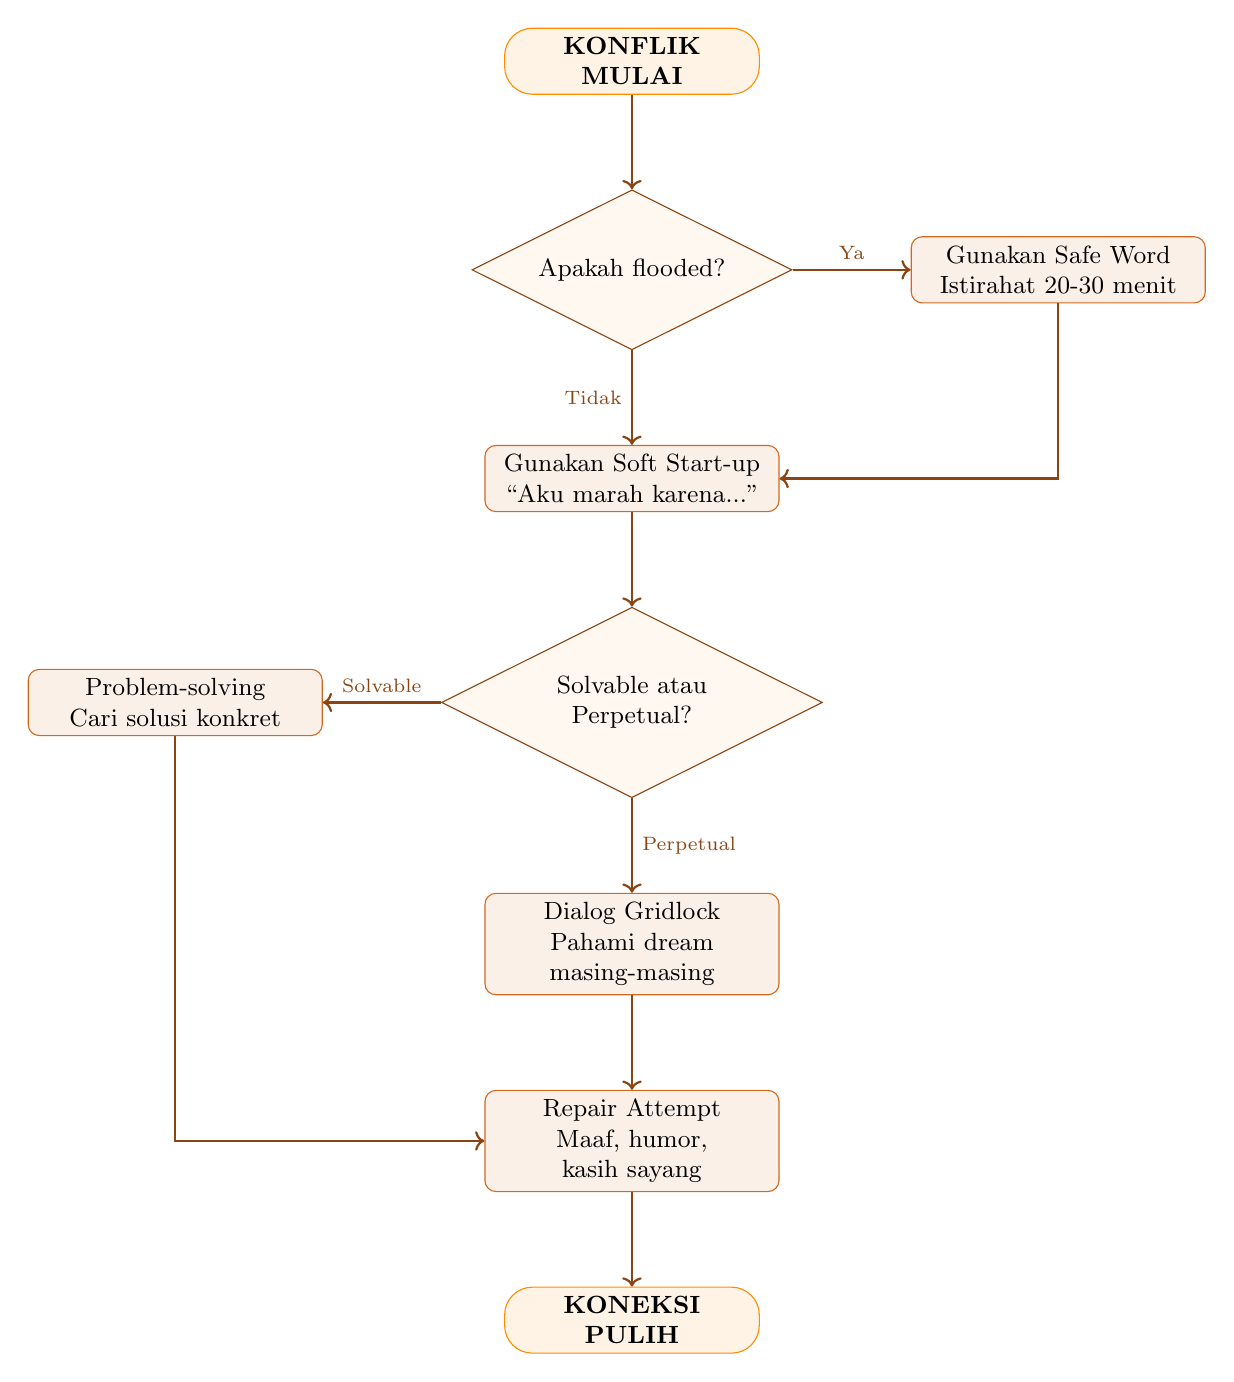
\begin{tikzpicture}[
    node distance=1.2cm,
    decision/.style={draw=primary, diamond, fill=lightbg, 
                     text width=2.8cm, align=center, aspect=2, font=\small},
    process/.style={draw=secondary, rectangle, fill=secondary!10,
                    text width=3.5cm, align=center, rounded corners, font=\small},
    startstop/.style={draw=accent, rectangle, fill=accent!10, rounded corners=10pt,
                      text width=3cm, align=center, font=\small\bfseries},
    arrow/.style={->, thick, primary}
]
    % Nodes
    \node[startstop] (start) {KONFLIK MULAI};
    \node[decision, below=of start] (flooded) {Apakah flooded?};
    \node[process, right=1.5cm of flooded] (break) {Gunakan Safe Word\\Istirahat 20-30 menit};
    \node[process, below=of flooded] (soft) {Gunakan Soft Start-up\\``Aku marah karena...''};
    \node[decision, below=of soft] (solvable) {Solvable atau\\Perpetual?};
    \node[process, left=1.5cm of solvable] (solve) {Problem-solving\\Cari solusi konkret};
    \node[process, below=of solvable] (manage) {Dialog Gridlock\\Pahami dream masing-masing};
    \node[process, below=of manage] (repair) {Repair Attempt\\Maaf, humor, kasih sayang};
    \node[startstop, below=of repair] (end) {KONEKSI PULIH};
    
    % Arrows
    \draw[arrow] (start) -- (flooded);
    \draw[arrow] (flooded) -- node[above, font=\scriptsize] {Ya} (break);
    \draw[arrow] (flooded) -- node[left, font=\scriptsize] {Tidak} (soft);
    \draw[arrow] (break) |- (soft);
    \draw[arrow] (soft) -- (solvable);
    \draw[arrow] (solvable) -- node[above, font=\scriptsize] {Solvable} (solve);
    \draw[arrow] (solvable) -- node[right, font=\scriptsize] {Perpetual} (manage);
    \draw[arrow] (solve) |- (repair);
    \draw[arrow] (manage) -- (repair);
    \draw[arrow] (repair) -- (end);
\end{tikzpicture}
\end{center}

\begin{tipbox}[Panduan Keputusan Cepat]
\textbf{$\square$ SAFE WORD Protocol:}
\begin{enumerate}[itemsep=0.1cm]
    \item Satu pihak menggunakan safe word
    \item Konflik \textbf{langsung stop} --- tidak ada ``tambahan kata terakhir''
    \item Pergi ke ruang terpisah
    \item Self-soothe 20-30 menit (jantung kembali normal)
    \item Kembali dan coba lagi dengan soft start-up
\end{enumerate}

\textbf{$\square$ Solvable vs Perpetual:}
\begin{itemize}[itemsep=0.1cm]
    \item \textbf{Solvable:} Masalah spesifik dengan situasi spesifik $\rightarrow$ Cari solusi konkret
    \item \textbf{Perpetual:} Perbedaan karakter/latar belakang $\rightarrow$ Dialog dengan empati
\end{itemize}
\end{tipbox}

\subsection{Template: Couple Agreement}

\begin{exercisebox}[Couple Agreement --- Kontrak Hubungan Kami]
\textbf{Kami, [Nama 1] dan [Nama 2], berkomitmen untuk:}

\vspace{0.3cm}
\textbf{KOMUNIKASI}
\begin{itemize}[itemsep=0.15cm]
    \item[$\square$] Melakukan State of the Union meeting setiap \rule{3cm}{0.4pt}
    \item[$\square$] Melakukan daily check-in minimal \rule{1cm}{0.4pt} menit per hari
    \item[$\square$] Safe word kami adalah: \rule{5cm}{0.4pt}
    \item[$\square$] Tidak menggunakan Four Horsemen dalam konflik
    \item[$\square$] Selalu melakukan repair attempt setelah konflik
\end{itemize}

\textbf{KONEKSI EMOSIONAL}
\begin{itemize}[itemsep=0.15cm]
    \item[$\square$] Update Love Maps secara rutin
    \item[$\square$] Quality time minimal \rule{1cm}{0.4pt} jam per minggu
    \item[$\square$] Date night setiap \rule{3cm}{0.4pt}
    \item[$\square$] Ritual koneksi harian: \rule{8cm}{0.4pt}
\end{itemize}

\textbf{KONFLIK}
\begin{itemize}[itemsep=0.15cm]
    \item[$\square$] Jika flooded: gunakan safe word, istirahat 20-30 menit
    \item[$\square$] Selalu gunakan soft start-up
    \item[$\square$] Terima pengaruh satu sama lain
    \item[$\square$] Jika perpetual problem: lakukan dialog gridlock
\end{itemize}

\textbf{KOMITMEN KHUSUS [Nama 1]:}
\begin{itemize}[itemsep=0.15cm]
    \item[$\square$] Aku akan \rule{10cm}{0.4pt}
    \item[$\square$] Saat aku butuh ruang, aku akan \rule{8cm}{0.4pt}
\end{itemize}

\textbf{KOMITMEN KHUSUS [Nama 2]:}
\begin{itemize}[itemsep=0.15cm]
    \item[$\square$] Aku akan \rule{10cm}{0.4pt}
    \item[$\square$] Saat aku cemas, aku akan \rule{8cm}{0.4pt}
\end{itemize}

\vspace{0.5cm}
\rule{6cm}{0.4pt} \hspace{1cm} \rule{6cm}{0.4pt}\\
[Nama 1] \hspace{4cm} [Nama 2]

\vspace{0.3cm}
Tanggal: \rule{3cm}{0.4pt}
\end{exercisebox}

\subsection{Template: Annual Relationship Review}

\begin{praktikbox}[Annual Relationship Review Template]
\textbf{Dilakukan setiap tahun (misal: anniversary)}

\vspace{0.3cm}
\textbf{BAGIAN 1: REFLEKSI TAHUN INI}

\textit{Hal-hal yang berhasil dengan baik:}
\begin{itemize}[itemsep=0.1cm]
    \item[$\square$] \\
    \item[$\square$] \\
    \item[$\square$] \\
\end{itemize}

\textit{Hal-hal yang perlu diperbaiki:}
\begin{itemize}[itemsep=0.1cm]
    \item[$\square$] \\
    \item[$\square$] \\
    \item[$\square$] \\
\end{itemize}

\textit{Momen terbaik tahun ini:} \hrulefill

\textit{Tantangan terbesar yang kita atasi:} \hrulefill

\textbf{BAGIAN 2: LOVE MAPS UPDATE}
\begin{itemize}[itemsep=0.1cm]
    \item[$\square$] Tujuan/aspirasi pasanganku saat ini:
    \item[$\square$] Beban terbesar yang dia pikul:
    \item[$\square$] Hal yang sedang dia khawatirkan:
    \item[$\square$] Apa yang membuatnya merasa paling hidup:
\end{itemize}

\textbf{BAGIAN 3: PERPETUAL PROBLEMS REVIEW}
\begin{itemize}[itemsep=0.1cm]
    \item[$\square$] Daftar perpetual problems kami:
    \begin{enumerate}
        \item 
        \item 
        \item 
    \end{enumerate}
    \item[$\square$] Bagaimana progress dialog gridlock untuk masing-masing?
    \item[$\square$] Apakah ada yang perlu approach baru?
\end{itemize}

\textbf{BAGIAN 4: GOALS TAHUN DEPAN}
\begin{itemize}[itemsep=0.1cm]
    \item[$\square$] Satu hal yang ingin kami capai bersama:
    \item[$\square$] Satu ritual baru yang ingin kami coba:
    \item[$\square$] Satu area hubungan yang ingin kami perkuat:
    \item[$\square$] Satu pengalaman baru yang ingin kami coba:
\end{itemize}
\end{praktikbox}

\section{Worksheets (Lembar Kerja)}

\subsection{Worksheet: Love Maps Questionnaire (20 Pertanyaan)}

\begin{exercisebox}[Love Maps Questionnaire]
\textbf{Petunjuk:} Jawablah pertanyaan-pertanyaan ini tentang pasanganmu. Tujuannya bukan untuk mendapat skor sempurna, tapi untuk melihat seberapa baik kamu mengenalnya.

\vspace{0.3cm}
\textbf{BAGIAN A: TENTANG KEHIDUPANNYA}

\begin{enumerate}[itemsep=0.2cm]
    \item Siapa sahabat terbaik pasanganmu saat ini? \hrulefill
    \item Siapa musuh bebuyutannya saat ini? \hrulefill
    \item Apa beban terbesar yang sedang dipikulnya? \hrulefill
    \item Apa yang paling membuatnya stres minggu ini? \hrulefill
    \item Apa yang paling membuatnya bahagia akhir-akhir ini? \hrulefill
\end{enumerate}

\textbf{BAGIAN B: TENTANG IMPIAN \& TAKUTNYA}

\begin{enumerate}[itemsep=0.2cm]
    \setcounter{enumi}{5}
    \item Apa impian terbesarnya yang belum pernah dia ceritakan? \hrulefill
    \item Apa ketakutan terbesarnya tentang masa depan? \hrulefill
    \item Apa yang ingin dia capai dalam 5 tahun ke depan? \hrulefill
    \item Apa pengalaman masa kecil yang paling berkesan baginya? \hrulefill
    \item Apa yang membuatnya merasa paling insecure? \hrulefill
\end{enumerate}

\textbf{BAGIAN C: TENTANG PREFERENSINYA}

\begin{enumerate}[itemsep=0.2cm]
    \setcounter{enumi}{10}
    \item Apa makanan favoritnya? \hrulefill
    \item Apa film/serial favoritnya saat ini? \hrulefill
    \item Apa musik yang paling dia suka? \hrulefill
    \item Apa aktivitas yang paling dia nikmati untuk melepas stres? \hrulefill
    \item Apa hadiah yang paling berarti baginya? \hrulefill
\end{enumerate}

\textbf{BAGIAN D: TENTANG HUBUNGAN}

\begin{enumerate}[itemsep=0.2cm]
    \setcounter{enumi}{15}
    \item Apa yang paling dia hargai dari hubungan kita? \hrulefill
    \item Apa yang membuatnya merasa paling dicintai? \hrulefill
    \item Apa yang paling dia butuhkan dariku saat stres? \hrulefill
    \item Apa yang dia harap aku lakukan lebih sering? \hrulefill
    \item Apa makna cinta baginya? \hrulefill
\end{enumerate}

\vspace{0.3cm}
\textbf{SKORING:}
\begin{itemize}[itemsep=0.1cm]
    \item 16-20 benar: \textbf{Excellent} --- Love Maps-mu sangat detail!
    \item 11-15 benar: \textbf{Good} --- Kamu mengenalnya dengan baik, tapi masih ada ruang untuk eksplorasi.
    \item 6-10 benar: \textbf{Fair} --- Perlu update Love Maps secara rutin.
    \item 0-5 benar: \textbf{Needs Work} --- Luangkan waktu untuk mengenalnya lebih dalam.
\end{itemize}
\end{exercisebox}

\subsection{Worksheet: Emotional Bank Account Tracker}

\begin{exercisebox}[Emotional Bank Account Tracker]
\textbf{Petunjuk:} Setiap interaksi positif adalah \textbf{deposit}, setiap interaksi negatif adalah \textbf{withdrawal}. Catat selama seminggu.

\vspace{0.3cm}
\textbf{MINGGU:} \rule{3cm}{0.4pt} \hspace{1cm} \textbf{BULAN:} \rule{3cm}{0.4pt}

\begin{center}
\renewcommand{\arraystretch}{1.4}
\begin{tabular}{|p{2cm}|p{4.5cm}|p{2cm}|p{4.5cm}|p{2cm}|}
\hline
\rowcolor{sagegreen!20}
\textbf{Hari} & \textbf{Deposit (+)} & \textbf{+Poin} & \textbf{Withdrawal (-)} & \textbf{-Poin} \\
\hline
Senin & & $\square$ 1 $\square$ 2 $\square$ 3 & & $\square$ 1 $\square$ 2 $\square$ 3 \\
\hline
Selasa & & $\square$ 1 $\square$ 2 $\square$ 3 & & $\square$ 1 $\square$ 2 $\square$ 3 \\
\hline
Rabu & & $\square$ 1 $\square$ 2 $\square$ 3 & & $\square$ 1 $\square$ 2 $\square$ 3 \\
\hline
Kamis & & $\square$ 1 $\square$ 2 $\square$ 3 & & $\square$ 1 $\square$ 2 $\square$ 3 \\
\hline
Jumat & & $\square$ 1 $\square$ 2 $\square$ 3 & & $\square$ 1 $\square$ 2 $\square$ 3 \\
\hline
Sabtu & & $\square$ 1 $\square$ 2 $\square$ 3 & & $\square$ 1 $\square$ 2 $\square$ 3 \\
\hline
Minggu & & $\square$ 1 $\square$ 2 $\square$ 3 & & $\square$ 1 $\square$ 2 $\square$ 3 \\
\hline
\end{tabular}
\end{center}

\vspace{0.3cm}
\textbf{RUMUS PERHITUNGAN:}
\begin{itemize}[itemsep=0.1cm]
    \item Deposit: $\square$ 1 (kecil), $\square$ 2 (sedang), $\square$ 3 (besar)
    \item Withdrawal: $\square$ 1 (kecil), $\square$ 2 (sedang), $\square$ 3 (besar)
\end{itemize}

\textbf{RASIO MINGGU INI:}
\begin{itemize}[itemsep=0.1cm]
    \item Total Deposit: \rule{2cm}{0.4pt}
    \item Total Withdrawal: \rule{2cm}{0.4pt}
    \item Rasio (Deposit:Withdrawal): \rule{3cm}{0.4pt}
\end{itemize}

\begin{tipbox}[Target Rasio]
\textbf{Target: 5:1 atau lebih tinggi} (5 deposit untuk setiap 1 withdrawal)

Jika rasio di bawah 3:1, hubungan berada dalam zona berbahaya.
\end{tipbox}
\end{exercisebox}

\subsection{Worksheet: Shared Meaning Assessment}

\begin{exercisebox}[Shared Meaning Assessment]
\textbf{Petunjuk:} Diskusikan bersama pasangan. Tidak ada jawaban benar atau salah --- yang penting adalah keselarasan.

\vspace{0.3cm}
\textbf{BAGIAN 1: PERAN DALAM HUBUNGAN}

\textit{Apa peran yang kita inginkan dalam hubungan?}
\begin{center}
\renewcommand{\arraystretch}{1.3}
\begin{tabular}{|p{4cm}|p{4cm}|p{5cm}|}
\hline
\rowcolor{primary!15}
\textbf{Area} & \textbf{[Nama 1]} & \textbf{[Nama 2]} \\
\hline
Pengambilan keputusan besar & & \\
\hline
Pengaturan keuangan & & \\
\hline
Tanggung jawab rumah tangga & & \\
\hline
Pengasuhan anak (jika ada) & & \\
\hline
Sosial/keluarga & & \\
\hline
\end{tabular}
\end{center}

\textbf{BAGIAN 2: NILAI \& VISI}

\textit{Seberapa selaras visi kita? (1-5, 5 = sangat selaras)}

\begin{itemize}[itemsep=0.2cm]
    \item[$\square$] Keuangan: [1] [2] [3] [4] [5]
    \item[$\square$] Karir dan ambisi: [1] [2] [3] [4] [5]
    \item[$\square$] Pola asuh: [1] [2] [3] [4] [5]
    \item[$\square$] Kehidupan sosial: [1] [2] [3] [4] [5]
    \item[$\square$] Spiritualitas/keyakinan: [1] [2] [3] [4] [5]
    \item[$\square$] Gaya hidup (kesehatan, olahraga): [1] [2] [3] [4] [5]
\end{itemize}

\textbf{BAGIAN 3: RITUAL KONEKSI}

\textit{Ritual apa yang sudah kita miliki?}
\begin{itemize}[itemsep=0.15cm]
    \item[$\square$] Morning ritual: \hrulefill
    \item[$\square$] Bedtime ritual: \hrulefill
    \item[$\square$] Greeting ritual (saat bertemu): \hrulefill
    \item[$\square$] Weekend ritual: \hrulefill
    \item[$\square$] Anniversary ritual: \hrulefill
\end{itemize}

\textit{Ritual baru yang ingin kita ciptakan:} \hrulefill
\end{exercisebox}

\subsection{Worksheet: Perpetual Problem Identification}

\begin{exercisebox}[Identifikasi Perpetual Problem]
\textbf{Petunjuk:} Identifikasi masalah yang muncul berulang kali dan selalu sulit diselesaikan.

\vspace{0.3cm}
\textbf{MASLAH 1}
\begin{itemize}[itemsep=0.15cm]
    \item Deskripsi masalah: \hrulefill
    \item Topik permukaan (apa yang kita pertengkarkan): \hrulefill
    \item Dream dalam konflik ini (di balik topik permukaan): \hrulefill
    \item Bagian [Nama 1]: \hrulefill
    \item Bagian [Nama 2]: \hrulefill
\end{itemize}

\textbf{MASLAH 2}
\begin{itemize}[itemsep=0.15cm]
    \item Deskripsi masalah: \hrulefill
    \item Topik permukaan (apa yang kita pertengkarkan): \hrulefill
    \item Dream dalam konflik ini (di balik topik permukaan): \hrulefill
    \item Bagian [Nama 1]: \hrulefill
    \item Bagian [Nama 2]: \hrulefill
\end{itemize}

\textbf{MASLAH 3}
\begin{itemize}[itemsep=0.15cm]
    \item Deskripsi masalah: \hrulefill
    \item Topik permukaan (apa yang kita pertengkarkan): \hrulefill
    \item Dream dalam konflik ini (di balik topik permukaan): \hrulefill
    \item Bagian [Nama 1]: \hrulefill
    \item Bagian [Nama 2]: \hrulefill
\end{itemize}

\begin{tipbox}[Panduan Identifikasi]
Perpetual problem biasanya:
\begin{itemize}[itemsep=0.1cm]
    \item Muncul berulang kali dengan pola yang sama
    \item Tidak pernah benar-benar terselesaikan
    \item Berkaitan dengan perbedaan karakter, latar belakang, atau nilai inti
    \item Saat dialog dengan baik, bukan untuk menyelesaikan, tapi untuk memahami
\end{itemize}
\end{tipbox}
\end{exercisebox}

\section{Emergency Protocols (Protokol Darurat)}

\subsection{Protokol: Ketika Flooding Terjadi}

\begin{warningbox}[EMERGENCY PROTOCOL --- FLOODING]
\textbf{STAGE 1: DETEKSI (Cek gejala flooding)}
\begin{itemize}[itemsep=0.1cm]
    \item[$\square$] Jantung berdebar lebih dari 100 bpm
    \item[$\square$] Napas pendek/cepat
    \item[$\square$] Otot tegang (rahang, bahu, tangan)
    \item[$\square$] Mulut kering
    \item[$\square$] Pikiran berkecamuk atau blank
    \item[$\square$] Ingin menyerang atau melarikan diri
    \item[$\square$] Tidak bisa mendengar/menerima informasi
\end{itemize}

\textbf{STAGE 2: STOP (Jika 3+ gejala terdeteksi)}
\begin{enumerate}[itemsep=0.15cm]
    \item[$\square$] Gunakan safe word atau katakan: ``Aku flooded, aku butuh break.''
    \item[$\square$] Tidak ada ``kata terakhir'' --- langsung stop
    \item[$\square$] Beri tahu kapan akan kembali: ``Aku akan kembali dalam 20-30 menit.''
    \item[$\square$] Pergi ke ruang terpisah
\end{enumerate}

\textbf{STAGE 3: SELF-SOOTHING (Selama break)}
\begin{itemize}[itemsep=0.1cm]
    \item[$\square$] Napas dalam 4-7-8 (tarik 4 detik, tahan 7, hembus 8)
    \item[$\square$] Meditasi atau mindfulness
    \item[$\square$] Olahraga ringan (jalan kaki)
    \item[$\square$] Mandi air hangat
    \item[$\square$] Dengar musik menenangkan
    \item[$\square$] \textbf{JANGAN}: Pikirkan argumen, merencanakan balas dendam, stalking medsos
\end{itemize}

\textbf{STAGE 4: RETURN (Setelah 20-30 menit)}
\begin{enumerate}[itemsep=0.15cm]
    \item[$\square$] Pastikan sudah tenang (jantung normal)
    \item[$\square$] Kembali ke pasangan sesuai janji
    \item[$\square$] Mulai dengan soft start-up
    \item[$\square$] Jika masih flooded, minta tambahan waktu dengan spesifik
\end{enumerate}
\end{warningbox}

\subsection{Protokol: Ketika Repair Attempts Gagal}

\begin{warningbox}[EMERGENCY PROTOCOL --- REPAIR ATTEMPTS GAGAL]
\textbf{Jika repair attempts kamu terus ditolak:}

\vspace{0.2cm}
\textbf{Langkah 1: Evaluasi}
\begin{itemize}[itemsep=0.1cm]
    \item[$\square$] Apakah waktunya tepat? (Jika pasangan masih flooded, tunggu)
    \item[$\square$] Apakah cara repair-nya sesuai dengan love language pasangan?
    \item[$\square$] Apakah kamu sudah mengakui bagian yang salah dengan spesifik?
\end{itemize}

\textbf{Langkah 2: Coba Pendekatan Berbeda}
\begin{itemize}[itemsep=0.1cm]
    \item[$\square$] Jika verbal gagal $\rightarrow$ Coba tulis surat/catatan
    \item[$\square$] Jika langsung gagal $\rightarrow$ Coba melalui aktivitas (cooking, jalan bareng)
    \item[$\square$] Jika serius gagal $\rightarrow$ Coba humor ringan atau affection fisik
\end{itemize}

\textbf{Langkah 3: Cek Deeper Issue}
\begin{itemize}[itemsep=0.1cm]
    \item[$\square$] Apakah ada masalah yang belum terselesaikan dari konflik sebelumnya?
    \item[$\square$] Apakah pasangan merasa tidak didengar/dipahami?
    \item[$\square$] Apakah ada trust issue yang mendalam?
\end{itemize}

\textbf{Langkah 4: Escalate}
\begin{itemize}[itemsep=0.1cm]
    \item[$\square$] Jadwalkan State of the Union meeting khusus untuk ini
    \item[$\square$] Pertimbangkan couples therapy jika pola ini berulang
    \item[$\square$] Jangan memaksa repair --- beri waktu, tapi tetap tunjukkan komitmen
\end{itemize}
\end{warningbox}

\subsection{Protokol: Ketika Mempertimbangkan Separation (Last Resort)}

\begin{warningbox}[EMERGENCY PROTOCOL --- LAST RESORT CHECKLIST]
\textbf{Sebelum memutuskan untuk berpisah, pastikan:}

\vspace{0.2cm}
\textbf{CHECKLIST TINDAKAN INTENSIF}

\textit{Sudahkah kalian:}
\begin{itemize}[itemsep=0.15cm]
    \item[$\square$] Melakukan State of the Union meeting rutin selama minimal 3 bulan?
    \item[$\square$] Mencoba couples therapy dengan profesional berlisensi?
    \item[$\square$] Menerapkan semua 7 Principles secara konsisten?
    \item[$\square$] Menerapkan safe word dan flooding protocol?
    \item[$\square$] Mencoba 30-day intensive connection program?
    \item[$\square$] Membaca dan menerapkan materi dari buku-buku rekomendasi?
    \item[$\square$] Memiliki support system (teman, keluarga, komunitas)?
\end{itemize}

\textbf{CHECKLIST EVALUASI HUBUNGAN}

\textit{Apakah masih ada:}
\begin{itemize}[itemsep=0.15cm]
    \item[$\square$] Fondness and admiration (meski kecil)?
    \item[$\square$] Friendship dasar?
    \item[$\square$] Shared meaning (visi bersama)?
    \item[$\square$] Kemauan dari kedua belah pihak untuk berusaha?
    \item[$\square$] Physical safety (tidak ada abuse)?
\end{itemize}

\textbf{JIKA ADA ABUSE (Fisik/Emosional):}
\begin{itemize}[itemsep=0.15cm]
    \item[$\square$] Prioritaskan keselamatan fisik dan emosionalmu
    \item[$\square$] Hubungi hotline darurat: 119 (Indonesia) atau hotline lokal
    \item[$\square$] Cari tempat aman
    \item[$\square$] Abuse bukan alasan untuk ``coba lagi'' --- safety first
\end{itemize}

\textbf{LANGKAH FINAL JIKA MEMUTUSKAN BERPISAH:}
\begin{enumerate}[itemsep=0.15cm]
    \item[$\square$] Konsultasi dengan counselor individual
    \item[$\square$] Siapkan support system
    \item[$\square$] Buat rencana praktis (finansial, tempat tinggal)
    \item[$\square$] Komunikasikan dengan jujur tapi sopan
    \item[$\square$] Terapkan closure ritual untuk berdua
\end{enumerate}
\end{warningbox}

\section{Resource Guide (Panduan Sumber Daya)}

\subsection{Further Reading (Buku yang Direkomendasikan)}

\begin{praktikbox}[Rekomendasi Bacaan]
\textbf{Foundational (Buku Utama):}
\begin{itemize}[itemsep=0.15cm]
    \item \textbf{The Seven Principles for Making Marriage Work} oleh John Gottman --- Buku dasar yang menjadi fondasi panduan ini
    \item \textbf{Wired for Dating} dan \textbf{Wired for Love} oleh Stan Tatkin --- Memahami attachment styles dan neuroscience relationship
    \item \textbf{Hold Me Tight} oleh Sue Johnson --- Emotionally Focused Therapy (EFT) untuk pasangan
    \item \textbf{Attached} oleh Amir Levine \& Rachel Heller --- Attachment theory dalam konteks dating modern
\end{itemize}

\textbf{Advanced Reading:}
\begin{itemize}[itemsep=0.15cm]
    \item \textbf{What Makes Love Last?} oleh John Gottman --- Tentang trust dan betrayal
    \item \textbf{The Relationship Cure} oleh John Gottman --- Emotional connection dalam semua relasi
    \item \textbf{Love Sense} oleh Sue Johnson --- Science of love attachment
    \item \textbf{Eight Dates} oleh John \& Julie Gottman --- Guided conversations untuk pasangan
    \item \textbf{Nonviolent Communication} oleh Marshall Rosenberg --- Komunikasi dengan empati
\end{itemize}

\textbf{For Specific Issues:}
\begin{itemize}[itemsep=0.15cm]
    \item \textbf{Come As You Are} oleh Emily Nagoski --- Sexual health dan intimacy
    \item \textbf{The Five Love Languages} oleh Gary Chapman --- Expressions of love
    \item \textbf{Getting the Love You Want} oleh Harville Hendrix --- Imago Relationship Therapy
    \item \textbf{Mating in Captivity} oleh Esther Perel --- Erotic intelligence dalam long-term relationship
\end{itemize}
\end{praktikbox}

\subsection{Kapan Harus Mencari Bantuan Profesional}

\begin{warningbox}[Tanda-tanda Butuh Terapis]
\textbf{Segera cari bantuan profesional jika:}
\begin{itemize}[itemsep=0.15cm]
    \item[$\square$] Four Horsemen dominan dan repair attempts gagal terus-menerus
    \item[$\square$] Salah satu atau kedua pihak sering flooded dan tidak bisa self-soothe
    \item[$\square$] Adanya kekerasan fisik atau ancaman kekerasan
    \item[$\square$] Adanya perselingkuhan (emotional atau fisik) yang belum terselesaikan
    \item[$\square$] Salah satu pihang mengancam perceraian/berpisah secara teratur
    \item[$\square$] Tidak ada fondness and admiration yang tersisa
    \item[$\square$] Konflik perpetual tidak bisa didialogkan dengan baik
    \item[$\square$] Tidak ada kemajuan setelah 3-6 bulan mencoba sendiri
\end{itemize}

\textbf{Jenis Terapis yang Direkomendasikan:}
\begin{itemize}[itemsep=0.1cm]
    \item \textbf{Gottman Method Therapist} --- Terlatih dalam metode Gottman
    \item \textbf{EFT Therapist} --- Emotionally Focused Therapy (ICEEFT certified)
    \item \textbf{PACT Therapist} --- Psychobiological Approach to Couple Therapy (Stan Tatkin)
    \item \textbf{Imago Therapist} --- Imago Relationship Therapy
\end{itemize}
\end{warningbox}

\subsection{Sumber Daya Online}

\begin{tipbox}[Resources Digital]
\textbf{Apps untuk Pasangan:}
\begin{itemize}[itemsep=0.1cm]
    \item \textbf{Gottman Card Decks} --- Prompts untuk conversation dan intimacy
    \item \textbf{Lasting} --- Marriage counseling app berbasis Gottman
    \item \textbf{Paired} --- Daily questions dan exercises untuk pasangan
    \item \textbf{Relish} --- Relationship coaching app
\end{itemize}

\textbf{Website \& Online Resources:}
\begin{itemize}[itemsep=0.1cm]
    \item \textbf{Gottman.com} --- Artikel, assessment, dan workshop
    \item \textbf{The Gottman Institute Blog} --- Research-based relationship advice
    \item \textbf{StanTatkin.com} --- Attachment and neuroscience of relationships
    \item \textbf{ICEEFT.com} --- Emotionally Focused Therapy resources
    \item \textbf{Psychology Today} --- Directory untuk mencari therapist lokal
\end{itemize}

\textbf{Assessment Online (Gratis):}
\begin{itemize}[itemsep=0.1cm]
    \item Love Languages Quiz (5lovelanguages.com)
    \item Attachment Style Quiz (various online resources)
    \item Gottman Love Lab assessments
\end{itemize}
\end{tipbox}

\vfill

\begin{center}

\begin{tikzpicture}
    \draw[primary, line width=3pt] (0,0) -- (12,0);
\end{tikzpicture}

\vspace{0.5cm}

{\Large\bfseries\color{primary} Selamat Membangun Hubungan yang Sehat!}

\vspace{0.3cm}

{\color{warmgray} ``Hubungan yang baik bukan tentang tidak pernah bertengkar,\\
tapi tentang bertengkar dengan cara yang memperkuat, bukan merusak.''}

\vspace{0.3cm}

{\color{warmgray} ``Tools dalam bab ini adalah kompas --- gunakan setiap saat\\
untuk menavigasi perjalanan cinta kalian.''}

\vspace{0.5cm}

{\Large\color{accent} $\bullet$ \hspace{0.3cm} $\bullet$ \hspace{0.3cm} $\bullet$}
\end{center}


\end{document}
